\pdfoutput=1

\documentclass[preprint,10pt]{elsarticle}
%\documentclass[preprint,10pt]{article}
%\documentclass[review]{siamart0216}
%\documentclass{siamart0216}

\usepackage{fullpage}
\usepackage[colorlinks=true]{hyperref}

\usepackage{amsmath,amssymb,amsfonts,amsthm}
\theoremstyle{definition}
\newtheorem{definition}{Definition}
\theoremstyle{lemma}
\newtheorem{lemma}{Lemma}
\newtheorem*{remark}{Remark}
\theoremstyle{theorem}
\newtheorem{theorem}{Theorem}
\theoremstyle{assumption}
\newtheorem{assumption}{Assumption}

\usepackage[titletoc,toc,title]{appendix}

\usepackage{array} 
\usepackage{listings}
\usepackage{mathtools}
\usepackage{pdfpages}
\usepackage[textsize=footnotesize,color=green]{todonotes}
\usepackage{bm}
\usepackage{bbm}

\usepackage{tikz}
\usepackage[normalem]{ulem}
\usepackage{hhline}

\usepackage{graphicx}
\usepackage{subfig}
\usepackage{color}

%% ====================================== graphics

\usepackage{pgfplots}
\usepackage{pgfplotstable}
\definecolor{markercolor}{RGB}{124.9, 255, 160.65}
\pgfplotsset{
compat=1.3,
width=10cm,
tick label style={font=\small},
label style={font=\small},
legend style={font=\small}
}

\usetikzlibrary{calc}
\usetikzlibrary{intersections} 

%%% START MACRO FOR ANNOTATION OF TRIANGLE WITH SLOPE %%%.
\newcommand{\logLogSlopeTriangle}[5]
{
    % #1. Relative offset in x direction.
    % #2. Width in x direction, so xA-xB.
    % #3. Relative offset in y direction.
    % #4. Slope d(y)/d(log10(x)).
    % #5. Plot options.

    \pgfplotsextra
    {
        \pgfkeysgetvalue{/pgfplots/xmin}{\xmin}
        \pgfkeysgetvalue{/pgfplots/xmax}{\xmax}
        \pgfkeysgetvalue{/pgfplots/ymin}{\ymin}
        \pgfkeysgetvalue{/pgfplots/ymax}{\ymax}

        % Calculate auxilliary quantities, in relative sense.
        \pgfmathsetmacro{\xArel}{#1}
        \pgfmathsetmacro{\yArel}{#3}
        \pgfmathsetmacro{\xBrel}{#1-#2}
        \pgfmathsetmacro{\yBrel}{\yArel}
        \pgfmathsetmacro{\xCrel}{\xArel}

        \pgfmathsetmacro{\lnxB}{\xmin*(1-(#1-#2))+\xmax*(#1-#2)} % in [xmin,xmax].
        \pgfmathsetmacro{\lnxA}{\xmin*(1-#1)+\xmax*#1} % in [xmin,xmax].
        \pgfmathsetmacro{\lnyA}{\ymin*(1-#3)+\ymax*#3} % in [ymin,ymax].
        \pgfmathsetmacro{\lnyC}{\lnyA+#4*(\lnxA-\lnxB)}
        \pgfmathsetmacro{\yCrel}{\lnyC-\ymin)/(\ymax-\ymin)} % THE IMPROVED EXPRESSION WITHOUT 'DIMENSION TOO LARGE' ERROR.

        % Define coordinates for \draw. MIND THE 'rel axis cs' as opposed to the 'axis cs'.
        \coordinate (A) at (rel axis cs:\xArel,\yArel);
        \coordinate (B) at (rel axis cs:\xBrel,\yBrel);
        \coordinate (C) at (rel axis cs:\xCrel,\yCrel);

        % Draw slope triangle.
        \draw[#5]   (A)-- node[pos=0.5,anchor=north] {}
                    (B)-- 
                    (C)-- node[pos=0.5,anchor=west] {#4}
                    cycle;
    }
}
%%% END MACRO FOR ANNOTATION OF TRIANGLE WITH SLOPE %%%.

\newcommand{\logLogSlopeTriangleNeg}[5]
{
    % #1. Relative offset in x direction.
    % #2. Width in x direction, so xA-xB.
    % #3. Relative offset in y direction.
    % #4. Slope d(y)/d(log10(x)).
    % #5. Plot options.

    \pgfplotsextra
    {
        \pgfkeysgetvalue{/pgfplots/xmin}{\xmin}
        \pgfkeysgetvalue{/pgfplots/xmax}{\xmax}
        \pgfkeysgetvalue{/pgfplots/ymin}{\ymin}
        \pgfkeysgetvalue{/pgfplots/ymax}{\ymax}

        % Calculate auxilliary quantities, in relative sense.
        \pgfmathsetmacro{\xArel}{#1}
        \pgfmathsetmacro{\yArel}{#3}
        \pgfmathsetmacro{\xBrel}{#1-#2}
        \pgfmathsetmacro{\yBrel}{\yArel}
        \pgfmathsetmacro{\xCrel}{\xArel}

        \pgfmathsetmacro{\lnxB}{\xmin*(1-(#1-#2))+\xmax*(#1-#2)} % in [xmin,xmax].
        \pgfmathsetmacro{\lnxA}{\xmin*(1-#1)+\xmax*#1} % in [xmin,xmax].
        \pgfmathsetmacro{\lnyA}{\ymin*(1-#3)+\ymax*#3} % in [ymin,ymax].
        \pgfmathsetmacro{\lnyC}{\lnyA+#4*(\lnxA-\lnxB)}
        \pgfmathsetmacro{\yCrel}{\lnyC-\ymin)/(\ymax-\ymin)} % THE IMPROVED EXPRESSION WITHOUT 'DIMENSION TOO LARGE' ERROR.

        % Define coordinates for \draw. MIND THE 'rel axis cs' as opposed to the 'axis cs'.
        \coordinate (A) at (rel axis cs:\xArel,\yArel);
        \coordinate (B) at (rel axis cs:\xBrel,\yBrel);
        \coordinate (C) at (rel axis cs:\xCrel,\yCrel);

        % Draw slope triangle.
        \draw[#5]   (A)-- node[pos=.5,anchor=south] {}
                    (B)-- 
                    (C)-- node[pos=0.5,anchor=west] {#4}
                    cycle;
    }
}
%%% END MACRO FOR ANNOTATION OF TRIANGLE WITH SLOPE %%%.

%%% START MACRO FOR ANNOTATION OF TRIANGLE WITH SLOPE %%%.
\newcommand{\logLogSlopeTriangleFlipNeg}[5]
{
    % #1. Relative offset in x direction.
    % #2. Width in x direction, so xA-xB.
    % #3. Relative offset in y direction.
    % #4. Slope d(y)/d(log10(x)).
    % #5. Plot options.

    \pgfplotsextra
    {
        \pgfkeysgetvalue{/pgfplots/xmin}{\xmin}
        \pgfkeysgetvalue{/pgfplots/xmax}{\xmax}
        \pgfkeysgetvalue{/pgfplots/ymin}{\ymin}
        \pgfkeysgetvalue{/pgfplots/ymax}{\ymax}

        % Calculate auxilliary quantities, in relative sense.
        %\pgfmathsetmacro{\xArel}{#1}
        %\pgfmathsetmacro{\yArel}{#3}
        \pgfmathsetmacro{\xBrel}{#1-#2}
        \pgfmathsetmacro{\yBrel}{#3}
        \pgfmathsetmacro{\xCrel}{#1}

        \pgfmathsetmacro{\lnxB}{\xmin*(1-(#1-#2))+\xmax*(#1-#2)} % in [xmin,xmax].
        \pgfmathsetmacro{\lnxA}{\xmin*(1-#1)+\xmax*#1} % in [xmin,xmax].
        \pgfmathsetmacro{\lnyA}{\ymin*(1-#3)+\ymax*#3} % in [ymin,ymax].
        \pgfmathsetmacro{\lnyC}{\lnyA+#4*(\lnxA-\lnxB)}
        \pgfmathsetmacro{\yCrel}{\lnyC-\ymin)/(\ymax-\ymin)} % THE IMPROVED EXPRESSION WITHOUT 'DIMENSION TOO LARGE' ERROR.

	\pgfmathsetmacro{\xArel}{\xBrel}
        \pgfmathsetmacro{\yArel}{\yCrel}

        % Define coordinates for \draw. MIND THE 'rel axis cs' as opposed to the 'axis cs'.
        \coordinate (A) at (rel axis cs:\xArel,\yArel);
        \coordinate (B) at (rel axis cs:\xBrel,\yBrel);
        \coordinate (C) at (rel axis cs:\xCrel,\yCrel);

        % Draw slope triangle.
        \draw[#5]   (A)-- node[pos=0.5,anchor=east] {#4}
                    (B)-- 
                    (C)-- node[pos=0.5,anchor=north] {1}
                    cycle;
    }
}
%%% END MACRO FOR ANNOTATION OF TRIANGLE WITH SLOPE %%%.


%%% START MACRO FOR ANNOTATION OF TRIANGLE WITH SLOPE %%%.
\newcommand{\logLogSlopeTriangleFlip}[5]
{
    % #1. Relative offset in x direction.
    % #2. Width in x direction, so xA-xB.
    % #3. Relative offset in y direction.
    % #4. Slope d(y)/d(log10(x)).
    % #5. Plot options.

    \pgfplotsextra
    {
        \pgfkeysgetvalue{/pgfplots/xmin}{\xmin}
        \pgfkeysgetvalue{/pgfplots/xmax}{\xmax}
        \pgfkeysgetvalue{/pgfplots/ymin}{\ymin}
        \pgfkeysgetvalue{/pgfplots/ymax}{\ymax}

        % Calculate auxilliary quantities, in relative sense.
        %\pgfmathsetmacro{\xArel}{#1}
        %\pgfmathsetmacro{\yArel}{#3}
        \pgfmathsetmacro{\xBrel}{#1-#2}
        \pgfmathsetmacro{\yBrel}{#3}
        \pgfmathsetmacro{\xCrel}{#1}

        \pgfmathsetmacro{\lnxB}{\xmin*(1-(#1-#2))+\xmax*(#1-#2)} % in [xmin,xmax].
        \pgfmathsetmacro{\lnxA}{\xmin*(1-#1)+\xmax*#1} % in [xmin,xmax].
        \pgfmathsetmacro{\lnyA}{\ymin*(1-#3)+\ymax*#3} % in [ymin,ymax].
        \pgfmathsetmacro{\lnyC}{\lnyA+#4*(\lnxA-\lnxB)}
        \pgfmathsetmacro{\yCrel}{\lnyC-\ymin)/(\ymax-\ymin)} % THE IMPROVED EXPRESSION WITHOUT 'DIMENSION TOO LARGE' ERROR.

	\pgfmathsetmacro{\xArel}{\xBrel}
        \pgfmathsetmacro{\yArel}{\yCrel}

        % Define coordinates for \draw. MIND THE 'rel axis cs' as opposed to the 'axis cs'.
        \coordinate (A) at (rel axis cs:\xArel,\yArel);
        \coordinate (B) at (rel axis cs:\xBrel,\yBrel);
        \coordinate (C) at (rel axis cs:\xCrel,\yCrel);

        % Draw slope triangle.
        \draw[#5]   (A)-- node[pos=0.5,anchor=east] {#4}
                    (B)-- 
                    (C)-- node[pos=0.5,anchor=south] {}
                    cycle;
    }
}
%%% END MACRO FOR ANNOTATION OF TRIANGLE WITH SLOPE %%%.



\usepackage{stmaryrd}


\renewcommand{\topfraction}{0.85}
\renewcommand{\textfraction}{0.1}
\renewcommand{\floatpagefraction}{0.75}

\newcommand{\vect}[1]{\ensuremath\boldsymbol{#1}}
\newcommand{\tensor}[1]{\underline{\bm{#1}}}
\newcommand{\del}{\triangle}
\newcommand{\curl}{\grad \times}
\renewcommand{\div}{\grad \cdot}

\newcommand{\bbm}[1]{\mathbbm{#1}}
\newcommand{\bs}[1]{\boldsymbol{#1}}
\newcommand{\equaldef}{\stackrel{\mathrm{def}}{=}}

\newcommand{\td}[2]{\frac{{\rm d}#1}{{\rm d}{\rm #2}}}
\newcommand{\pd}[2]{\frac{\partial#1}{\partial#2}}
\newcommand{\pdd}[2]{\frac{\partial^2#1}{\partial#2^2}}
\newcommand{\pdn}[3]{\frac{\partial^{#3}#1}{\partial#2^{#3}}}
\newcommand{\mb}[1]{\mathbf{#1}}
\newcommand{\mbb}[1]{\mathbb{#1}}
\newcommand{\mc}[1]{\mathcal{#1}}
\newcommand{\snor}[1]{\left| #1 \right|}
\newcommand{\nor}[1]{\left\| #1 \right\|}
\newcommand{\LRp}[1]{\left( #1 \right)}
\newcommand{\LRs}[1]{\left[ #1 \right]}
\newcommand{\LRa}[1]{\left\langle #1 \right\rangle}
\newcommand{\LRb}[1]{\left| #1 \right|}
\newcommand{\LRc}[1]{\left\{ #1 \right\}}
\newcommand{\LRceil}[1]{\left\lceil #1 \right\rceil}
\newcommand{\LRl}[1]{\left. #1 \right|}

%\newcommand{\cond}[1]{\kappa\LRp{#1}}
\newcommand{\cond}[2]{\nor{#1}_{#2}\nor{{#1}^{-1}}_{#2}}


\newcommand{\Grad} {\ensuremath{\nabla}}
\newcommand{\Div} {\ensuremath{\nabla\cdot}}
\newcommand{\jump}[1] {\ensuremath{\llbracket#1\rrbracket}}
\newcommand{\avg}[1] {\ensuremath{\LRc{\!\{#1\}\!}}}

\newcommand{\Oh}{{\Omega_h}}
\renewcommand{\L}{L^2\LRp{\Omega}}
\newcommand{\LK}{L^2\LRp{D^k}}
\newcommand{\LdK}{L^2\LRp{\partial D^k}}
\newcommand{\Dhat}{\widehat{D}}
\newcommand{\Lhat}{L^2\LRp{\Dhat}}

\newcommand{\eval}[2][\right]{\relax
  \ifx#1\right\relax \left.\fi#2#1\rvert}

\def\etal{{\it et al.~}}

\newcommand{\note}[1]{{\color{blue}{#1}}}

\newcommand{\LinfDk}{L^{\infty}\LRp{D^k}}

\newcommand{\diag}[1]{{\rm diag}\LRp{#1}}

\newcommand{\Ksub}{K_{\rm sub}}

\newcolumntype{C}[1]{>{\centering\let\newline\\\arraybackslash\hspace{0pt}}m{#1}}

%% d in integrand
\newcommand*\diff[1]{\mathop{}\!{\mathrm{d}#1}}


\makeatletter
\renewcommand\d[1]{\mspace{6mu}\mathrm{d}#1\@ifnextchar\d{\mspace{-3mu}}{}}
\makeatother

%\date{}
%\author{Jesse Chan}
%\title{On discretely entropy conservative discontinuous Galerkin methods}
\graphicspath{{./figs/}}


\begin{document}

%\maketitle

\begin{frontmatter}
\title{On discretely entropy conservative and entropy stable discontinuous Galerkin methods}

\author[rice]{Jesse Chan\corref{cor1}}
\ead{Jesse.Chan@caam.rice.edu}
\address[rice]{Department of Computational and Applied Mathematics, Rice University, 6100 Main St, Houston, TX, 77005}

\begin{abstract}
High order methods based on diagonal-norm summation by parts operators can be shown to satisfy a discrete conservation or dissipation of entropy for nonlinear systems of hyperbolic PDEs \cite{fisher2013high, carpenter2014entropy}.  These methods can also be interpreted as nodal discontinuous Galerkin methods with diagonal mass matrices \cite{gassner2016split, gassner2016well, wintermeyer2017entropy, chen2017entropy}.  In this work, we describe how to construct discretely entropy conservative schemes to a more general class of DG methods using flux differencing, quadrature-based projections, and specific DG differentiation operators.  This approach also recovers existing methods for Burgers' equation involving dense norm and generalized SBP operators without boundary nodes \cite{fernandez2014generalized, ranocha2016summation, ranocha2017extended}.  Numerical experiments confirm the stability and high order accuracy of the proposed methods for the one-dimensional compressible Euler equations.  
\end{abstract}
\end{frontmatter}

%\tableofcontents

\section{Introduction}

Numerical simulations in engineering increasingly require higher accuracy without sacrificing computational efficiency.  Because they are more accurate than low order methods per degree of freedom for sufficiently regular solutions, high order methods provide one avenue towards improving fidelity in numerical simulations while maintaining reasonable computational costs.  High order methods which can accomodate unstructured meshes are desirable for problems with complex geometries, and among such methods, high order discontinuous Galerkin (DG) methods are particularly well-suited to the solution of time-dependent hyperbolic problems on modern computing architectures \cite{hesthaven2007nodal, klockner2009nodal}.  

The accuracy of high order methods can be attributed in part to their low numerical dissipation and dispersion compared to low order schemes \cite{ainsworth2004dispersive}.  This accuracy has made them advantageous for the simulation of wave propagation \cite{hesthaven2007nodal, wilcox2010high}.  However, while high order methods can be applied in a stable manner to linear wave propagation problems, instabilities are observed when applying them to nonlinear hyperbolic problems.  This is contrast to low order schemes, whose high numerical dissipation tends to apply a stabilizing effect \cite{wang2013high}.  As a result, most high order schemes for nonlinear conservation laws typically require additional stabilization procedures, including  filtering \cite{hesthaven2007nodal}, slope limiting \cite{krivodonova2007limiters}, artificial viscosity \cite{persson2006sub}, and polynomial de-aliasing through over-integration \cite{kirby2003aliasing}.  Moreover, stabilized numerical methods can still fail, requiring user intervention or heuristic modifications to achieve non-divergent solutions.  

For linear wave propagation problems, semi-discretely energy stable numerical methods can be constructed, even in the presence of curvilinear coordinates or variable coefficients \cite{warburton2013low, chan2016weight1, chan2016weight2, chan2017weight}.  This semi-discrete stability implies that, under a stable timestep restriction (CFL condition), discrete solutions do not suffer from non-physical growth in time.  However, for nonlinear systems of conservation laws, traditional methods do not admit theoretical proofs of semi-discrete stability.  This was addressed for low order methods with the introduction of discretely entropy conservative and entropy stable finite volume schemes by Tadmor \cite{tadmor1987numerical}.   These schemes rely on a specific entropy conservative flux which satisfies a condition involving the entropy variables and entropy potential, and were extended to low order finite volume methods on unstructured grids in \cite{ray2016entropy}.  High order entropy stable methods were also developed for structured grids in \cite{fjordholm2012arbitrarily} based on an entropy conservative essentially non-oscillatory (ENO) reconstruction.  

The extension of entropy conservative schemes to unstructured high order methods was done much more recently for the compressible Euler and Navier-Stokes equations in \cite{fisher2013high, carpenter2014entropy} based on a spectral collocation approach on tensor product elements, which can also be interpreted as a mass-lumped DG spectral element (DG-SEM) scheme.  The proof of entropy conservation relies on the presence of a diagonal mass matrix, the summation by parts (SBP) property \cite{gassner2013skew}, and  a concept referred to as flux differencing.  Similar entropy-stable schemes have been constructed for the shallow water and MHD equations \cite{gassner2016well,  wintermeyer2017entropy, winters2017uniquely}.  More recently, high order entropy conservative and entropy stable schemes were extended to unstructured triangular meshes in \cite{chen2017entropy} using the split-form methodology of \cite{gassner2016split} and multi-dimensional SBP operators \cite{hicken2016multidimensional, crean2017high}.  

To the authors knowledge, the construction of unstructured high order entropy conservative and entropy stable schemes  has required diagonal norm SBP operators.  We refer to DG methods with these properties as diagonal norm SBP-DG methods.  Entropy stable high order finite element and DG methods which do not fall under the diagonal norm SBP-DG category have been proposed \cite{hughes1986new}, but the proofs are often given at the continuous level, relying on exact integration or the chain rule, neither of which holds discretely.

On the other hand, while entropy conservative schemes can be constructed by combining flux differencing with diagonal norm SBP operators, this restricts methods to specific choices of basis and quadrature.  Appropriate diagonal norm SBP operators are straightforward to construct on tensor product elements based on a DG-SEM discretization.  Diagonal-norm SBP operators can also be constructed for triangles and tetrahedra \cite{chin1999higher,  hicken2016multidimensional, chen2017entropy}; however, the number of nodal points for such operators is typically greater than the dimension of the natural polynomial approximation space.  Furthermore, to the author's knowledge, appropriate point sets have only been constructed for $N \leq 4$ in three dimensions \cite{zhebel2014comparison}, and the construction of high order diagonal norm SBP-DG methods has not yet been performed for uncommon elements such as pyramids \cite{chan2016orthogonal}.  

This work focuses on the construction of entropy conservative high order DG schemes for systems of conservation laws.  In order to generalize beyond diagonal norm SBP-DG methods, we will consider non-lumped (dense) mass matrices and more general quadrature rules (e.g.\ rules without boundary points, rules with more points than the dimension of the corresponding approximation space), which are also related to dense norm and generalized SBP operators \cite{fernandez2014generalized, ranocha2016summation, ranocha2017extended, ranocha2017comparison}.  The work presented in this manuscript is intended to serve as a stepping stone to the construction of entropy stable DG methods on general elements in two and three dimensions.  We will present proofs of discrete entropy stability in terms of integrals and $L^2$ projections, which we assume are computed using an appropriate quadrature rule.  We stress that, while this work adopts a continuous notation involving integrals rather than discrete sums, the proofs rely only on properties of quadrature-based integration and quadrature-based $L^2$ projection.  

The outline of the paper is as follows: Section~\ref{sec:intro} will briefly review the construction of entropy conservative diagonal norm SBP-DG methods on a single element.  Section~\ref{sec:ecdg} will describe how to construct analogous entropy conservative methods on single element in a continuous setting.  Section~\ref{sec:ecdg2} will discuss extensions to multiple elements, including comparisons of different coupling terms and entropy stable fluxes.  Finally, Section~\ref{sec:num} presents numerical results which verify the high order accuracy and discrete entropy conservation of the proposed methods.  We note that, for simplicity and clarity of presentation, the proposed methods, proofs, and numerical experiments are given in one dimension.  However, the extension to multiple dimensions (including simplicial elements) is straightforward and will be described in an upcoming manuscript.  


%\note{The construction of such operators on non-tensor product elements (such as simplices or pyramids) is non-trivial.} \cite{hicken2016multidimensional, chen2017entropy}.  \note{Constructing such operators for non-polynomial spaces (such as splines) is also difficult within the current framework.}


\section{Entropy conservative diagonal norm SBP-DG methods}
\label{sec:intro}

We will begin by reviewing continuous entropy theory and existing high order methods which are provably entropy conservative at the discrete level.  These methods were introduced in \cite{fisher2013high, carpenter2014entropy} for tensor product elements, though we adopt more general methods of proof introduced recently in \cite{gassner2017br1, chen2017entropy}.  The proofs are based on diagonal norm SBP operators, which can be derived from a nodal discontinuous Galerkin framework through the collocation of nodal points and quadrature points \cite{gassner2013skew}.

\subsection{Entropy stability for systems of hyperbolic PDEs}

%\note{Specify that all analysis is done in 1D but is extendable to higher dimensions!!  For simplicity and clarity of presentation, we will begin by focusing on the case $d = 1$.  }

We consider systems of nonlinear conservation laws in one dimension with $n$ variables
\begin{align}
%\pd{\bm{u}}{t} + \sum_{k=1}^d \pd{\bm{f_k(\bm{u})}}{x} &= 0, \qquad \bm{u}(x,t) = (u_1(x,t),\ldots,u_n(x,t)).
\pd{\bm{u}}{t} + \pd{\bm{f(\bm{u})}}{x} &= 0, \qquad \bm{u}(x,t) = (u_1(x,t),\ldots,u_n(x,t)).
\label{eq:pde}
\end{align}
where the fluxes $f(\bm{u})$ are smooth functions of the vector of conservative variables $\bm{u}({x},t)$.  The Jacobian matrix $\bm{A}(\bm{u})$ is defined entrywise as
\[
%\LRp{\bm{A}_k(\bm{u})}_{ij} = \LRp{\pd{\bm{f}_k(\bm{u})}{\bm{u}_j}}_i.
\LRp{\bm{A}(\bm{u})}_{ij} = \LRp{\pd{\bm{f}(\bm{u})}{{u}_j}}_i.
\]
We are interested in systems for which there exists a convex entropy function $U(\bm{u})$ such that  
\begin{equation}
%U''(\bm{u})\bm{A}_k(\bm{u}) = \LRp{U''(\bm{u}) \bm{A}_k(\bm{u})}^T.
U''(\bm{u})\bm{A}(\bm{u}) = \LRp{U''(\bm{u}) \bm{A}(\bm{u})}^T.
\label{eq:entropysym}
\end{equation}
For systems with convex entropy functions, one can define entropy variables $\bm{v} = U'(\bm{u})$.  The convexity of the $U(\bm{u})$ guarantees that the mapping between conservative and entropy variables is invertible.  

It can be shown (see, for example, \cite{mock1980systems}) that (\ref{eq:entropysym}) is equivalent to the existence of an entropy flux function $F(\bm{u})$ such that
\[
\bm{v}^T \pd{\bm{f}}{\bm{u}} = \pd{F(\bm{u})}{\bm{u}}^T.
\]
The flux function and entropy flux function are further related through the so-called entropy potential $\psi$ 
\[
%\psi_k(\bm{v}) = \bm{v}^T\bm{f}_k(\bm{u}(\bm{v})) - F_k(\bm{u}(\bm{v})), \qquad \psi_k'(\bm{v}) = \bm{f}_k(\bm{u}(\bm{v})).
\psi(\bm{v}) = \bm{v}^T\bm{f}(\bm{u}(\bm{v})) - F(\bm{u}(\bm{v})), \qquad \psi'(\bm{v}) = \bm{f}(\bm{u}(\bm{v})).
\]

When $\bm{u}$ is smooth, multiplying (\ref{eq:pde}) on the left by $\bm{v}^T = U'(\bm{u})^T$, applying the definition of the entropy flux and using the chain rule yields the conservation of entropy
\[
\pd{U(\bm{u})}{t} + \pd{F(\bm{u})}{{x}} = 0.
\]
More generally, it can be shown that physically relevant solutions of (\ref{eq:pde}) (defined as the limiting solution for an appropriately defined vanishing viscosity) satisfy the entropy inequality
\[
\pd{U(\bm{u})}{t} + \pd{F(\bm{u})}{{x}} \leq 0.  
\]

We assume now that the domain is the interval $[-1,1]$.  Integrating the entropy inequality over this interval and using the definition of the entropy potential then yields
\begin{equation}
\int_{-1}^1 \pd{U(\bm{u})}{t} + \left.\LRp{\bm{v}^T\bm{f}(\bm{u}(\bm{v}))-\psi(\bm{v})}\right|_{-1}^1 \leq 0.  
\label{eq:consentropy}
\end{equation}
The focus of this work is the construction of methods which satisfy a discrete analogue of this entropy inequality.  We begin by reviewing existing discretely entropy conservative methods based on diagonal norm SBP operators. 

\subsection{Entropy conservative methods based on diagonal-norm SBP operators}

Let ${x}_i \in [-1,1]$ denote the $(N+1)$ point Gauss-Lobatto-Legendre (GLL) quadrature rule with positive weights $w_1,\ldots,w_{N+1}$, which integrates exactly polynomials of degree $(2N-1)$.  Let $\ell_i(x)$ denote the nodal Lagrange basis defined at GLL points, and define the differentiation matrix $\bm{D}$ be defined as 
\[
\bm{D}_{ij} = \pd{\ell_j(x_i)}{x}.
\]
The matrix $\bm{D}$ maps from nodal values of a polynomial to nodal values of its derivative.  We also define the mass matrix $\bm{M}$
\[
\bm{M}_{ij} = \int_{-1}^1 \ell_i(x)\ell_j(x)\diff{x} \approx \sum_{k} \ell_i(x_k)\ell_j(x_k) w_k = \delta_{ij} w_i,
\]
where the equality holds only approximately due to the inexactness of GLL quadrature for polynomials of degree $2N$.  For this choice of quadrature, the Kronecker property $\ell_j(x_i) = \delta_{ij}$ implies that $\bm{M}$ is a diagonal matrix whose entries are simply the quadrature weights.  

The mass and derivative matrices may be used to define the diagonal norm SBP operator $\bm{S} = \bm{M}\bm{D}$, with the summation-by-parts property 
\[
\bm{S} = \bm{B} - \bm{S}^T, \qquad \bm{B}_{ij} = \begin{cases}
-1 &i = j = 1 \\
1 &i = j = N+1 \\
0 &\text{otherwise}
\end{cases}.
\]
This property is simply a restatement of integration by parts, using that the derivative of $\ell_j(x)$ is a polynomial of degree $(N-1)$ and that GLL quadrature is exact for polynomials of degree $(2N-1)$.  

We seek a polynomial approximation to the solution $\bm{u}(x)$ of (\ref{eq:pde}).  A DG formulation in the ``strong form'' \cite{hesthaven2007nodal} is given as
\[
\int_{-1}^1\LRp{ \pd{\bm{u}}{t} + \pd{\bm{f}(\bm{u})}{x}}\bm{w} + \left.\LRp{\bm{f}^* - \bm{f}(\bm{u})} \bm{w}\right|_{-1}^1 = 0, \qquad \forall \bm{w}\in V_h,
\]
where $\bm{w}(x)$ is a vector-valued test function.
Here, $\bm{f}^*$ is some numerical flux used for the weak imposition of boundary or continuity conditions.  

We derive a DG-SEM approximation by evaluating the above integrals using GLL quadrature.  We furthermore assume that the vector solution is approximated using a nodal basis at GLL points 
\[
\bm{u}(x,t) = \sum_{j=1}^{N+1} \bm{u}_j(t)\ell_j(x).  
\]
The resulting semi-discrete system yields a nodal collocation scheme for each (vector-valued) degree of freedom $\bm{u}_i$ 
\[
%\pd{\bm{u}_i}{t} + \sum_{j=1}^{N+1}\LRp{\LRp{\bm{D}\otimes \bm{I}}_{ij}\bm{f}(\bm{u}_j) +\LRp{\LRp{\bm{M}^{-1}\bm{B}} \otimes \bm{I}}_{ij}(\bm{f}_i^* - \bm{f}(\bm{u}_i))} = 0, \qquad i = 1,\ldots,N+1.
\pd{\bm{u}_i}{t} + \sum_{j=1}^{N+1}\LRp{\LRp{\bm{D}_{ij}\otimes \bm{I}}\bm{f}(\bm{u}_j) +\LRp{\LRp{\bm{M}^{-1}\bm{B}}_{ij}\otimes \bm{I} }(\bm{f}_j^* - \bm{f}(\bm{u}_j))} = 0, \qquad i = 1,\ldots,N+1,
\]
where $\bm{f}^*$ is the vector whose entries consist of evaluations of the numerical flux at boundary nodes and zeros at interior nodes.  

This formulation conserves the quantities $\bm{u}_i$, but does not satisfy a discrete analogue of the statement of entropy conservation (\ref{eq:consentropy}) except in specific cases.  Entropy conservative schemes may be constructed based on the SBP property and a ``flux differencing'' approach \cite{gassner2016split} involving a definition of entropy conservative/stable fluxes given by Tadmor \cite{tadmor1987numerical}.  
\begin{definition}
Let $\bm{f}_S(\bm{u}_L,\bm{u}_R)$ be a bivariate function which is symmetric and consistent with the flux function $\bm{f}(\bm{u})$
\[
\bm{f}_S(\bm{u}_L,\bm{u}_R) = \bm{f}_S(\bm{u}_R,\bm{u}_L), \qquad \bm{f}_S(\bm{u},\bm{u}) = \bm{f}(\bm{u})
\]
The numerical flux $\bm{f}_S(\bm{u}_L, \bm{u}_R)$ is entropy conservative if, for entropy variables $\bm{v}_L = \bm{v}(\bm{u}_L), \bm{v}_R = \bm{v}(\bm{u}_R)$
\[
\LRp{\bm{v}_L - \bm{v}_R}^T \bm{f}_S(\bm{u}_L,\bm{u}_R) = (\psi_L - \psi_R), \qquad \psi_L = \psi(\bm{v}(\bm{u}_L)), \quad \psi_R = \psi(\bm{v}(\bm{u}_R)).  
\]
Similarly, a flux $\bm{f}_S(\bm{u}_L, \bm{u}_R)$ is referred to as entropy stable if $\LRp{\bm{v}_L - \bm{v}_R}^T \bm{f}_S(\bm{u}_L,\bm{u}_R) \leq (\psi_L - \psi_R)$.
\label{def:tadmor}
\end{definition}
An entropy conservative diagonal norm SBP-DG method can then be derived by modifying the flux derivative as follows
\begin{equation}
\pd{\bm{u}_i}{t} + \sum_{j=1}^{N+1}\LRp{\LRp{2\bm{D}_{ij}\otimes \bm{I}}\bm{f}_S(\bm{u}_i,\bm{u}_j) +\LRp{\LRp{\bm{M}^{-1}\bm{B}}_{ij}\otimes \bm{I}}(\bm{f}_j^* - \bm{f}(\bm{u}_j))}= 0.
\label{eq:dgsem}
\end{equation}
The replacement of the derivative of the flux function with flux differencing allows one to prove that (\ref{eq:dgsem}) conserves a discrete entropy \cite{gassner2017br1,chen2017entropy}.  We reproduce these proofs here, as we will refer to them in following sections.  
\begin{theorem}
The nodal collocation method (\ref{eq:dgsem}) is discretely entropy conservative in the sense that
\[
\bm{1}^T\LRp{\bm{M}\pd{U(\bm{u})}{t} + \bm{B}\LRp{\bm{v}^T\bm{f}^* - \bm{\psi}}} = 0,
\]
where $\bm{1}$ denotes the vector of ones and $\bm{\psi}_i = \psi(\bm{v}_i)$ is the entropy potential evaluated in terms of the nodal values $\bm{u}_i$.  
\label{thm:dgsem}
\end{theorem}
\begin{proof}
In this proof, we assume the matrices $\bm{M}$, $\bm{D}$, $\bm{B}$ are understood to act component-wise on the vector of solution degrees of freedom $\bm{u}$ and drop the explicit Kronecker product for simplicity of notation.  Let $\bm{v}_i = \bm{v}(\bm{u}_i)$ denote nodal values of the entropy variables.  We multiply (\ref{eq:dgsem}) by $\LRp{\bm{M}\bm{v}}^T$.  
Using the fact that $\bm{M}$ is diagonal, the time derivative term can be manipulated to 
\[
\bm{v}^T\bm{M}\pd{\bm{u}}{t} = \sum_{i=1}^{N+1} \bm{M}_{ii} \bm{v}_i^T \pd{\bm{u}_i}{t} = \sum_{i=1}^{N+1} \bm{M}_{ii} \pd{U(\bm{u}_i)}{t} = \bm{1}^T\bm{M}\pd{U(\bm{u}_i)}{t},
\]
where we have used continuity in time to arrive at the point-wise relation 
\[
\bm{v}^T \pd{\bm{u}}{t} = \pd{U(\bm{u})}{\bm{u}}^T \pd{\bm{u}}{t} = \pd{U(\bm{u})}{t}.
\]

The spatial derivative term can be manipulated using the summation by parts property $\bm{M}\bm{D} = \bm{S} = \bm{B}-\bm{S}^T$
\begin{align}
\sum_{i,j=1}^{N+1} \bm{v}_i^T 2 \bm{M}\bm{D}_{ij}\bm{f}_S(\bm{u}_i,\bm{u}_j) &= \sum_{i,j=1}^{N+1} \bm{v}_i^T (\bm{S} + \bm{B} - \bm{S}^T)_{ij}\bm{f}_S(\bm{u}_i,\bm{u}_j) \nonumber\\
&= \sum_{i,j=1}^{N+1} \bm{S}_{ij}\bm{v}_i^T \bm{f}_S(\bm{u}_i,\bm{u}_j) - \bm{S}_{ji}\bm{v}_i^T \bm{f}_S(\bm{u}_i,\bm{u}_j) + \bm{B}_{ij}\bm{v}_i^T \bm{f}_S(\bm{u}_i,\bm{u}_j). \label{eq:sbpentropy}
\end{align}
Rearranging indices and using symmetry of $\bm{f}_S(\bm{u}_i,\bm{u}_j)$ then yields that
\begin{align*}
\sum_{i,j=1}^{N+1} \bm{S}_{ij}\bm{v}_i^T \bm{f}_S(\bm{u}_i,\bm{u}_j) - \bm{S}_{ji}\bm{v}_i^T \bm{f}_S(\bm{u}_i,\bm{u}_j) &= \sum_{i,j=1}^{N+1} \bm{S}_{ij} \LRp{\bm{v}_i - \bm{v}_j}^T\bm{f}_S(\bm{u}_i,\bm{u}_j)\\
&= \sum_{i,j=1}^{N+1} \bm{S}_{ij} \LRp{\bm{\psi}_i-\bm{\psi}_j} = -\bm{1}^T \bm{S}\bm{\psi} = -\bm{1}^T\bm{B}\bm{\psi},
\end{align*}
where we have used $\bm{S}\bm{1} = 0$ and the summation by parts property in the last line.  

Using that $\bm{B}$ is diagonal, combining the latter term in (\ref{eq:sbpentropy}) with boundary terms involving the numerical flux yields
\[
\sum_{i,j = 1}^{N+1} \bm{B}_{ij}\bm{v}_i^T \bm{f}_S(\bm{u}_i,\bm{u}_j) + \bm{v}_i^T\bm{B}_{ij}\LRp{\bm{f}_j^* - \bm{f}(\bm{u}_j)} = \bm{1}^T\bm{B} \LRp{\bm{v}^T \bm{f}^*},
\]
where we have used the consistency of $\bm{f}_S(\bm{u},\bm{u}) = \bm{f}(\bm{u})$.  Putting these components together results in a discrete statement of the conservation of entropy (\ref{eq:consentropy}).   
%Combining everything results in a discrete statement of the conservation of entropy (\ref{eq:consentropy}) 
%\[
%\bm{1}^T\LRp{\bm{M}\pd{U(\bm{u})}{t} + \bm{B}\LRp{\bm{v}^T\bm{f}^* - \bm{\psi}}} = 0.
%\]
\end{proof}
We note that, unlike the continuous proof of entropy conservation, the proof of discrete entropy conservation avoids the use of the chain rule, which does not hold in general at the discrete level.  This proof of entropy conservation can also be extended beyond a single element by by taking $\bm{f}^*$ to be the entropy conservative flux $f_S(u_L,u_R)$ at the interface between two elements \cite{carpenter2014entropy, gassner2017br1, chen2017entropy}.
%specifying appropriate simultaneous approximation terms (SBP-SAT).  
Similarly, employing an entropy stable flux at element interfaces results in an entropy stable method which satisfies a global entropy inequality.  

It is important to emphasize that conservation of entropy does not, in general, imply stability of the numerical scheme unless the solution satisfies additional constraints.  For example, the transformation between conservative and entropy variables for the compressible Euler and Navier-Stokes equations is well-defined only if the density and pressure are positive, and steps must be taken in any numerical scheme to guarantee that the discrete solution satisfies such constraints.  For DG methods, this is most commonly done using bound and positivity-preserving limiters \cite{zhang2010positivity, zhang2012maximum}.  


\section{Entropy conservative DG methods on a single element}
\label{sec:ecdg}

In this section, we focus on constructing entropy conservative DG schemes for general choices of basis and quadrature.  These include (as special cases) dense norm SBP operators and generalized SBP (GSBP) operators which do not contain boundary points.  Difficulties in generalizing entropy conservative SBP-DG schemes present themselves primarily in two areas: the assumption of a diagonal mass matrix, which is used in the proof of entropy stability, and the generalization of flux differencing to a continuous formulation.  We address both areas of difficulty by extending the entropy conservative DG-SEM scheme (\ref{eq:dgsem}) from a discrete formulation to a continuous formulation involving flux differencing.  We prove that the continuous scheme is entropy conservative (stable) on a single element in the following sections, and describe how to apply the proposed methods to produce energy conservative formulations of Burgers' equation as an illustrative example.  

% to a larger class of quadratures and choices of basis.  Additionally, we prove that the generalized scheme is entropy conservative (stable) on multiple elements in the following sections.  

%We will get around these difficulties for dense-norm DG methods by satisfying three requirements for entropy stability
%\begin{itemize}
%\item $\bm{D}\bm{1} = 0$ for use of the flux formulation.  
%\item For some norm matrix $\bm{W}$, $\bm{W}\bm{D} = \bm{B}-\bm{D}^T\bm{W}$ where $\bm{B}$ is a suitably defined boundary operator.
%\item Contraction with the \textit{projection} of the entropy variables.  
%\end{itemize}

\subsection{Notation}

%\note{Fix}

We assume that the domain $\Omega$ is a finite interval, which is decomposed into non-overlapping elements $D^k$ of size $h$.  We define the reference element $\widehat{D} = [-1,1]$, such that $D^k$ is the image of $\widehat{D}$ under an affine mapping $x = \Phi^k(\widehat{x})$.  We define an approximation space using degree $N$ polynomials on the reference element
\[
P^N\LRp{\widehat{D}} = \LRc{\widehat{x}^i, \quad \widehat{x} \in \widehat{D}, \quad 0\leq i \leq N}.
\]
where we define $N_p = {\rm dim}\LRp{P^N\LRp{\widehat{D}}}$ (with $N_p = N+1$ in one dimension).  
%We define an approximation space over the reference element $\widehat{D}$ as the space of degree $N$ polynomials 
%\[
%P^N\LRp{\widehat{D}} = \LRc{\widehat{x}^i, \qquad 0\leq i \leq N}.
%\]
%We will approximate solution components over each element $D^k$ using 
% $V_h\LRp{D^k}$, which we define as the composition of the mapping $\bm{\Phi}^k$ and $P^N\LRp{\widehat{D}}$
%\[
%V_h\LRp{D^k} = \bm{\Phi}^k \circ V_h\LRp{\widehat{D}}.
%\]
We approximate the solution over a physical element by mapping $P^N\LRp{\widehat{D}}$ to $D^k$ under $\Phi^k$, and define the global approximation space $V_h$ as the direct sum of local approximation spaces
\[
P^N\LRp{D^k} =  {\Phi}^k \circ P^N\LRp{\widehat{D}}, \qquad V_h = \bigoplus_{k}P^N\LRp{D^k}.
\]
We define the $L^2$ norm and inner products over the element $D^k$ and the surface of the element $\partial D^k$
\[
\LRp{\bm{u},\bm{v}}_{D^k} = \int_{D^k} \bm{u}\cdot\bm{v}\diff{x} =  \int_{\widehat{D}} \bm{u}\cdot\bm{v} J^k \diff{\widehat{x}}, \qquad \nor{\bm{u}}^2_{D^k} = (\bm{u},\bm{u})_{D^k}, \qquad \LRa{\bm{u},\bm{v}}_{\partial D^k} = \int_{\partial D^k} \bm{u} \cdot \bm{v} \diff{x},
\]
where $J^k$ is the determinant of the Jacobian of $\Phi^k$.  
We also define the local $L^2$ projection operator $\Pi_N: L^2(D^k)\rightarrow P^N(D^k)$ such that
\[
\LRp{\Pi_N u,v}_{D^k} = \LRp{u,v}_{D^k}, \qquad \forall v\in P^N\LRp{D^k}.  
\]
In one dimension, $D^k$ is some interval and the $L^2$ inner product over the surface $\LRc{-1,1}$ reduces to 
\[
\LRa{u,v}_{\partial D^k} = u(x_L)v(x_L) + u(x_R)v(x_R).
\]  
However, the presented proofs in this work will not directly utilize this simplification in order to remain generalizable to higher dimensions in a straightforward manner.  

In typical implementations, integrals and inner products are  approximated using a quadrature rule consisting of $N_q \geq N_p$ points $\widehat{x}_i$ and weights $w_i$ over the reference element $\widehat{D}$, such that
\[
\LRp{u,v}_{D^k} \coloneqq \sum_{i=1}^{N_q} u(\widehat{x}_i)v(\widehat{x}_i)w_i J^k.     
\]
This also defines an analogous quadrature-based $L^2$ projection operator.  We emphasize that, throughout this work, we will only use properties of quadrature-based inner products and projection operators.  We assume only that the quadrature is sufficiently accurate to integrate degree $(2N-1)$ polynomials, such that integration by parts holds for any two polynomials on the reference element, while allowing for quadratures with an arbitrary number of points.  

%\note{specify assumptions - integrate polynomials of degree $N$ on the reference element exactly, such that integration by parts holds.  Add footnote that we can also generalize to the under-integrated case.  }

Finally, we define the jump and average of discontinuous functions across element interfaces.  Let $D^{k,+}$ denote the neighboring element of across a face $f$ of $D^k$, and let $u^+$ denote the values of $u$ on $D^{k,+}$.  The jump of $u$ across $f$ on $D^k$ is then defined as
\[
\jump{u} = u^+ - u, \qquad \avg{u} = \frac{u^+ + u}{2}.
\]
The jump and average of vector fields are defined component-wise using the jumps and averages of components.  When the face $f$ lies on the boundary, we define $u^+ = u$ such that $\jump{u} = 0$ and $\avg{u} = u$ on $\partial \Omega$.


\subsection{A continuous interpretation of flux differencing}

In this section, we offer a continuous interpretation of flux differencing \cite{fisher2013high,gassner2017br1,chen2017entropy}, which also encompasses the split form methodology proposed in \cite{gassner2016split}.  This interpretation will guide the construction of entropy conservative DG schemes.  

Assume that $\bm{f}_S(\bm{u}_L,\bm{u}_R)$ is the symmetric and consistent two-point flux defined in (\ref{def:tadmor}).  Consider the bilinear function
\[
\bm{f}_S\LRp{\bm{u}(x),\bm{u}(y)}, \qquad x, y \in \mathbb{R}.  
\]
Flux differencing can be interpreted as differentiating $\bm{f}_S\LRp{\bm{u}(x),\bm{u}(y)}$ along one coordinate $x$, then evaluating the result with $y=x$
\begin{equation}
\pd{\bm{f}(\bm{u}(x))}{x} \Longrightarrow 2\left.\pd{\bm{f}_S\LRp{\bm{u}(x),\bm{u}(y)}}{x}\right|_{y=x}.
\label{eq:fluxdiff}
\end{equation}
It was shown in \cite{chen2017entropy} that flux differencing provides a consistent approximation of the flux derivative $\pd{\bm{f}(\bm{u})}{x}$.  
%Since the two-point flux is consistent, 

%\subsubsection{Illustration using Burgers' equation}

It is helpful to first understand flux differencing as a method for recovering split formulations.  We illustrate this using the one-dimensional Burgers equation on domain $ [-1,1]$, which is given in conservative form as 
\[
\pd{u}{t} + \pd{f(u)}{x} = 0, \qquad f(u) = \frac{1}{2}u^2.
\]
%An alternative form of the Burgers' equation can be derived by taking a convex combination of the conservative and non-conservative forms of the spatial term
%\begin{equation}
%\pd{u}{t} + \frac{1}{3}\LRp{\pd{u^2}{x} + u\pd{u}{x}} = 0.
%\label{eq:burgerssplit}
%\end{equation}
Assuming smooth $u$, Burgers' equation conserves a square entropy $U(\bm{u}) = u^2/2$.   This can be shown by multiplying by $u$, integrating over $[-1,1]$, using the chain rule in time and space, and integrating by parts to arrive at
\begin{equation}
\frac{1}{2}\pd{}{t}\int_{-1}^1{u}^2 = -\left.\frac{u^3}{3}\right|_{-1}^1.
\label{eq:burgersconservation}
\end{equation}

An alternative rewriting of the Burgers' equation is the split formulation \cite{gassner2013skew, ranocha2017extended}, which may be also be recovered using flux differencing under the following two-point flux
\[
f_S(u_L,u_R) = \frac{1}{6}(u_L^2 + u_Lu_R + u_R^2).
\]
Applying (\ref{eq:fluxdiff}) yields the split form of Burgers' equation
\[
2\left.\pd{f_S(u(x),u(y))}{x}\right|_{y=x} = \frac{1}{3}\left.\pd{\LRp{u(x)^2 + u(x)u(y) + u(y)^2}}{x}\right|_{y=x} = \frac{1}{3}\LRp{\pd{u^2}{x} + u\pd{u}{x}}.
\]
We note that recovering the split-form of Burgers' equation relies on the property
%\footnote{This is also the reason why the factor of $2$ is necessary when using flux differentiation (\ref{eq:fluxdiff}); the differentiation of terms which depend only on $y$ vanish, \note{finish...}.}
that 
\[
\pd{\LRp{u(y)^2}}{x} = u(y)^2\pd{\LRp{1}}{x} = 0.  
\]
Thus, recovery of the split form can be achieved by using flux differencing in combination with any differential operator $D$ such that $D1 = 0$.  

\subsection{Discrete differential operators and weighted integration by parts}

While both the conservative and split forms of Burgers' equation are equivalent at the continuous level (assuming smoothness of $u$), they are not equivalent at the discrete level.  Suppose now that the solution is approximated by $u \in P^N\LRp{\widehat{D}}$ on the reference element.  Since $f(u) = u^2/2 \not\in P^N\LRp{\widehat{D}}$ for general choices of $u$, it is not possible to differentiate $f(u)$ exactly without prior knowledge of the form of the nonlinearity.  Indeed, it is more common to first project $f(u)$ to $P^N\LRp{\widehat{D}}$, then differentiate, such that the discrete scheme is equivalent to solving for $u \in P^N\LRp{\widehat{D}}$ such that
\[
\int_{-1}^1 \LRp{\pd{u}{t} + \pd{\Pi_N f(u)}{x}}w \diff{x}  
%\int_{-1}^1 \LRp{\pd{u}{t} +D_N f(u)}w \diff{x} 
=0, \qquad \forall w \in P^N\LRp{\widehat{D}}.  
\]
This scheme does not, in general, conserve the square entropy $u^2/2$.  %Moreover, if $\Pi_N$ is computed using quadrature, rewriting the scheme into this form suggests that de-aliasing techniques based on over-integration hit a ``bottleneck'', due to the fact that increasing quadrature accuracy only increases the accuracy of the projection \cite{kirby2003aliasing}.  

We can derive a semi-discrete Galerkin scheme which conserves energy using flux differencing and a discrete differentiation operator $D_N$, which is inspired by the SBP operators introduced in \cite{chen2017entropy}.  Define $H^1\LRp{\widehat{D}}$ as the Sobolev space over $\widehat{D}$
\begin{equation}
\nor{u}_{H^1\LRp{\widehat{D}}}^2 = \nor{u}_{L^2\LRp{\widehat{D}}}^2 + \nor{\pd{u}{x}}_{L^2\LRp{\widehat{D}}}^2, \qquad H^1\LRp{\widehat{D}} = \LRc{ u \in L^2\LRp{\widehat{D}}, \qquad \nor{u}_{H^1\LRp{\widehat{D}}} < \infty}.\label{eq:sobolev}
\end{equation}
Because functions $u \in H^1\LRp{\widehat{D}}$ admit a well-defined boundary trace \cite{brenner2007mathematical}, we can define the following discrete differential operator as a map from $H^1$ to $P^N$:
\begin{definition}
\label{def:dgd}
Let $w(x)$ be a continuous and bounded function on $\widehat{D}$.  Define $D_N: H^1\LRp{\widehat{D}}\rightarrow P^N\LRp{\widehat{D}}$ such that, for $u\in H^1\LRp{\widehat{D}}$, 
\begin{align}
&\LRp{D_N u, vw}_{\widehat{D}} = \LRp{\pd{ \Pi_N u}{x},vw}_{\widehat{D}}\nonumber \\
&+ \frac{1}{2}{\LRa{{u - \Pi_N u}, vw{n}_x}}_{\partial \widehat{D}} + \frac{1}{2}\LRa{u - \Pi_Nu ,\Pi_N\LRp{vw}{n}_x }_{\widehat{D}}, \qquad \forall v\in P^N\LRp{\widehat{D}},
\end{align}
where ${n}_x$ is the $x$-component of the outward normal vector.  
\end{definition}
This operator satisfies a form of integration by parts, which is summarized by the following lemma:
\begin{lemma}
\label{lemma:dgd_local}
The linear operator $D_N$ satisfies a ``weighted'' integration by parts property with respect the $L^2$ inner product and any bounded real-valued function $w(x)$ 
\[
\LRp{D_N u, wv}_{\widehat{D}} = \LRa{u,wv{n}_x}_{\partial \widehat{D}} - \LRp{u,D_N (w v)}_{\widehat{D}}.
\]
\end{lemma}
\begin{proof}
Integrating the left hand side by parts gives
\[
-\LRp{\pd{ \Pi_N (vw)}{x},u}_{\widehat{D}} + \frac{1}{2}{\LRa{{u - \Pi_N u}, vw{n}_x}}_{\partial \widehat{D}} + \frac{1}{2}\LRa{u + \Pi_Nu ,\Pi_N\LRp{vw}{n}_x }_{\partial \widehat{D}}, \qquad \forall v\in P^N\LRp{\widehat{D}}.
\]
Rearranging boundary terms yields
\[
-\LRp{\pd{ \Pi_N (vw)}{x},u}_{\widehat{D}} + \frac{1}{2}\LRa{vw + \Pi_N(vw) , u{n}_x }_{\partial \widehat{D}}  - \frac{1}{2}\LRa{vw - \Pi_N (vw), \Pi_N u {n}_x}_{\partial \widehat{D}}.  
\]
Adding and subtracting $\LRa{vw,u{n}_x}_{\partial \widehat{D}}$ completes the proof.
\end{proof}

Direct computations also show that $\LRp{D_N 1,vw}_{\widehat{D}} = 0$ for all bounded weights $w(x)$ and $\forall v \in P^N\LRp{\widehat{D}}$.  Thus, we can apply (\ref{eq:fluxdiff}) with $D_N$ to construct a discrete formulation for Burgers' equation
\begin{align}
\LRp{\pd{u}{t},v} + \frac{1}{3}\LRp{D_N u^2 + uD_Nu,v} &= \LRp{\pd{u}{t},v}_{\widehat{D}} + \frac{1}{3}\LRp{D_N u^2,v}_{\widehat{D}} + \frac{1}{3}\LRp{D_Nu,uv}_{\widehat{D}},
%\LRp{\pd{u}{t},v}_{\widehat{D}} + \frac{1}{3}\LRp{\pd{\Pi_N u^2}{x},v}_{\widehat{D}} + \frac{1}{3}\LRp{D_Nu,uv}_{\widehat{D}}
\qquad \forall v\in P^N\LRp{\widehat{D}}.
\label{eq:burgersdiscrete}
\end{align}
To show this formulation is discretely energy conservative, we take $v=u$ and use Lemma~\ref{lemma:dgd_local} to cancel volume terms, yielding
\[
\frac{1}{2}\pd{}{t}\LRp{u,u}_{\widehat{D}} = \frac{1}{2}\pd{}{t}\nor{u}^2_{\widehat{D}} = -\frac{1}{3}\LRa{u^2,u}_{\partial \widehat{D}},
\]
which is a discrete analogue of the conservation of energy (\ref{eq:burgersconservation}) for smooth solutions.  This is equivalent to the skew-symmetric split formulation described in \cite{gassner2013skew}; however, as noted in \cite{chen2017entropy}, it can be derived from flux differencing without explicit knowledge of the skew form.  We will show later in Section~\ref{sec:recovery} that a natural extension of this formulation to multiple elements recovers the weak form of the scheme introduced in \cite{ranocha2017extended}.  

%We note that the $L^2$ projection appears within the boundary terms.  While this may not pose a significant problem on one element, in the case of multiple elements, it introduces an all-to-all coupling between degrees of freedom on elements which share a face \cite{fernandez2016simultaneous}.  In the following section, we describe an alternative choice of discrete differential operator $D$ inspired by Chen and Shu \cite{chen2017entropy} which avoids this problem of increased bandwidth while maintaining properties which are necessary to guarantee provably discrete entropy conservation.  


\subsection{Conservation of entropy on one element}
\label{sec:ec}
While flux differencing can be used to recover split formulations, it can also be used to construct entropy stable formulations which do not correspond to skew-symmetric splittings.  In this section we will show that, for any sufficiently accurate quadrature rule and appropriate numerical flux function, it is possible to construct discretizations which satisfy a discrete equivalent of conservation of entropy (\ref{eq:consentropy}).  

For the proof, we will need the following assumption:
\begin{assumption}
The numerical flux function $\bm{f}_S$ admits an absolutely convergent expansion of the form 
\[
\bm{f}_S(x,y) = \sum_{i=1}^{\infty} \bm{f}_i(x) \bm{g}_i(y), 
\]
where $\bm{f}_i, \bm{g}_i$ are real and bounded for appropriate values of $x,y$ over each element.  
\label{eq:assumption}
\end{assumption}
The precise definition of what constitutes ``appropriate values of $x,y$'' depends on the physical problem.  For example, the flux functions for the compressible Euler equations require positivity constraints on the inputs, which are outlined in more detail in Section~\ref{sec:num}.  This assumption is satisfied, for example, by $\bm{f}_S$ which are real analytic and thus admit a Taylor expansion in the two arguments.  In \ref{appendix:A}, we argue that this assumption also holds for the flux functions $\bm{f}_S$ considered in this work for the Burgers' and compressible Euler equations, assuming the solution satisfies physical bound constraints.  However, we emphasize that this assumption is not required in the computation implementations of the proposed methods, and that it may also be possible to relax these conditions on $\bm{f}_S$.  

We now introduce a discretization for the nonlinear system of conservation laws (\ref{eq:pde}) on the reference element $\widehat{D}$: find $\bm{u}\in P^N\LRp{\widehat{D}}$ such that
\begin{equation}
\LRp{\pd{\bm{u}}{t},\bm{w}}_{\widehat{D}} + \LRp{\left.\LRp{2D_N \bm{f}_S(\bm{u}_{\bm{v}}(x),\bm{u}_{\bm{v}}(y))}\right|_{y=x},\bm{w}}_{\widehat{D}}+ \LRa{\bm{f}^*-\bm{f}(\bm{u}_{\bm{v}}),\bm{w}{n}_x}_{\partial \widehat{D}} = 0, \qquad \bm{w}\in P^N\LRp{\widehat{D}},
\label{eq:ecdg_oneelem}
\end{equation}
where $\bm{f}^*$ is a numerical flux used to impose boundary conditions weakly, and $\bm{u}_{\bm{v}}(x),\bm{u}_{\bm{v}}(y)$ are evaluations of $\bm{u}$ in terms of the projections of entropy variables $\bm{v}(\bm{u}(x))$ 
\begin{equation}
%\bm{u}_{\bm{v}}(x) = \bm{u}(\Pi_N\bm{v}(\bm{u}(x))), \qquad \bm{u}_{\bm{v}}(y) = \bm{u}(\Pi_N\bm{v}(\bm{u}(y))).
\bm{u}_{\bm{v}}(x) = \bm{u}\LRp{(\Pi_N\bm{v})(x)}.
\label{eq:projectedentropyvars}
\end{equation}


\begin{theorem}
\label{lemma:ec1}
Let Assumption~\ref{eq:assumption} hold on $\widehat{D}$.  The formulation (\ref{eq:ecdg_oneelem})
 %and (\ref{eq:ecdg_oneelem_mat}) are
 is semi-discretely entropy conservative in the sense that
\[
\LRp{\pd{U(\bm{u})}{t},1}_{\widehat{D}} =  \LRa{\psi,1{n}_x}_{\partial \widehat{D}}-\LRa{{\bm{f}^*, \Pi_N\bm{v}}{n}_x}_{\partial \widehat{D}}.
\]
\end{theorem}
\begin{proof}
We take the test function $\bm{w}$ to be the projection of the entropy variables.  On the left hand side, we may use the fact that, under a method of lines discretization, 
\[
\bm{u}(x,t) = \sum_{j=1}^{N_p} \bm{u}_j(t) \phi_j(x), \qquad \pd{\bm{u}(x,t)}{t} \in P^N\LRp{\widehat{D}}.
\]
Thus, testing with $\Pi_N \bm{v}$ and assuming continuity in time yields 
\[
\LRp{\pd{\bm{u}}{t}, \Pi_N \bm{v}(\bm{u})}_{\widehat{D}} = \LRp{\pd{\bm{u}}{t},\bm{v}(\bm{u})}_{\widehat{D}} = \LRp{\pd{U(\bm{u})}{t},1}_{\widehat{D}}, \qquad \forall \bm{u}\in P^N\LRp{\widehat{D}}.
\]
%Let $\bm{v}_q$ denote the entropy variables evaluated in terms of the conservative variables at quadrature points.  Then, the same argument involving the time term can be shown using matrix notation by testing with $\bm{v} = {\bm{P}_q\bm{v}_q}$,
%\[
%\LRp{\bm{P}_q\bm{v}_q}^T\bm{M}\pd{\bm{u}}{t} = \bm{v}_q^T\bm{W}\bm{V}_q\bm{M}^{-1}\bm{M}\pd{\bm{u}}{t} = \bm{1}^T \bm{W} {\rm diag}(\bm{v}_q) \pd{\bm{u}_q}{t} = \bm{1}^T \bm{W} \pd{U(\bm{u}_q)}{t},
%\]
%where we have assumed continuity in time, and have used that $\bm{W}$ is diagonal.  
For the spatial derivative, we expand $\bm{f}_S$ out using Assumption~\ref{eq:assumption} and apply Lemma~\ref{lemma:dgd_local}
\begin{align*}
&\LRp{\left.\LRp{D_N \sum_{i=1}^{\infty}\bm{f}_i(\bm{u}_{\bm{v}}(x))\bm{g}_i(\bm{u}_{\bm{v}}(y))}\right|_{y=x}, \Pi_N\bm{v}(x)}_{\widehat{D}} = \sum_{i=1}^{\infty} \LRp{{D_N \bm{f}_i(\bm{u}_{\bm{v}})}, {\bm{g}_i(\bm{u}_{\bm{v}})\Pi_N\bm{v} }}_{\widehat{D}}\\
&= \sum_{i=1}^{\infty}\LRa{\bm{f}_i(\bm{u}_{\bm{v}}) \bm{g}_i(\bm{u}_{\bm{v}}),\Pi_N\bm{v}{n}_x}_{\partial \widehat{D}}  - \LRp{ \bm{f}_i(\bm{u}_{\bm{v}}), D_N \LRp{\bm{g}_i\Pi_N\bm{v} }}_{\widehat{D}}\\
&= \LRa{\bm{f}_S(\bm{u}_{\bm{v}},\bm{u}_{\bm{v}}), \Pi_N\bm{v}(x){n}_x}_{\partial \widehat{D}}  - \LRp{\left.\LRp{D_N \LRp{\bm{f}_S(\bm{u}_{\bm{v}}(y),\bm{u}_{\bm{v}}(x))\Pi_N\bm{v}(x)} }\right|_{y=x},1}_{\widehat{D}}\\
%&= \LRa{\bm{f}_S(\bm{u}_{\bm{v}},\bm{u}_{\bm{v}}), \Pi_N\bm{v}(x)}_{\partial \widehat{D}}  - \LRp{\left.\LRp{D_N \LRp{\bm{f}_S(\bm{u}_{\bm{v}}(x),\bm{u}_{\bm{v}}(y))\Pi_N\bm{v}(x)} }\right|_{y=x},1}_{\widehat{D}}\\
&= \LRa{\bm{f}(\bm{u}_{\bm{v}}), \Pi_N\bm{v}(x){n}_x}_{\partial \widehat{D}}  - \LRp{\left.\LRp{D_N\LRp{\bm{f}_S(\bm{u}_{\bm{v}}(x),\bm{u}_{\bm{v}}(y))\Pi_N\bm{v}(x)} }\right|_{y=x},1}_{\widehat{D}},
\end{align*}
where we have used the linearity of $D_N$ in the first step and the symmetry and consistency of $\bm{f}_S$ in the third and last steps.  
%where $\Pi_N^x, \Pi_N^y$ denote $L^2$ projections taken with respect to the $x$ and $y$ coordinates, respectively.  
Noting that 
\[
\left.\LRp{D_N \bm{f}_S(\bm{u}_{\bm{v}}(x),\bm{u}_{\bm{v}}(y))}\right|_{y=x}\bm{v}(x) = \left.\LRp{D_N \LRp{\bm{f}_S(\bm{u}_{\bm{v}}(x),\bm{u}_{\bm{v}}(y))\bm{v}(y)}}\right|_{y=x},
\]
the volume terms can be manipulated to yield
\begin{align*}
%&\LRp{\left.\LRp{D_N \LRp{\bm{f}_S(\bm{u}(\Pi_N\bm{v}(x)),\bm{u}(\Pi_N\bm{v}(y)))\LRp{\Pi_N\bm{v}(y)-\Pi_N\bm{v}(x)} }}\right|_{y=x},1}_{\widehat{D}} \\
&\LRp{\left.\LRp{D_N \LRp{\bm{f}_S(\bm{u}_{\bm{v}}(x),\bm{u}_{\bm{v}}(y))\LRp{\Pi_N\bm{v}(y)-\Pi_N\bm{v}(x)} }}\right|_{y=x},1}_{\widehat{D}} \\
&= \LRp{ \left.\LRp{D_N\LRp{\psi(y)-\psi(x) }}\right|_{y=x},1}_{\widehat{D}} = \LRp{-D_N \psi(x),1}_{\widehat{D}} = \LRa{-\psi,1}_{\partial \widehat{D}},
\end{align*}
where we have used Definition~\ref{def:tadmor} in going from the first to second integral and Lemma~\ref{lemma:dgd_local} in the final step.  
\end{proof}

We see that, in the proof of Theorem~\ref{lemma:ec1}, recovering the time derivative of entropy on the left hand side requires testing with the projection of the entropy variables.  For diagonal norm SBP-DG methods, $L^2$ projection and nodal interpolation are equivalent, which implies that evaluating the flux $\bm{f}_S$ using point-wise nodal values of the solution satisfies the entropy conservation condition given in Definition~\ref{def:tadmor}.  %Diagonal norm SBP-DG methods can be further simplified by noting that the projection operator reduces to a nodal interpolation operator.  

In general, the projection of the entropy variables does not agree with their point-wise evaluation.  However, the entropy conservation condition given in Definition~\ref{def:tadmor} holds so long as the flux is evaluated in a manner consistent with the projected entropy variables used to recover the time derivative of entropy.  This motivates (\ref{eq:projectedentropyvars}) as a non-standard way of evaluating the flux, which is the primary difference between the construction of entropy conservative schemes for diagonal norm SBP-DG methods and more general DG methods.  

Finally, we note that, while projected entropy variables can be used to build entropy conservative DG methods, the evaluation $\bm{u}\LRp{\Pi_N \bm{v}}$ can be sensitive to differences between $\bm{v}$ and $\Pi_N \bm{v}$, which are illustrated numerically and described in more detail in Section~\ref{sec:instab}.  

\begin{remark}
In the proof of Theorem~\ref{lemma:ec1}, Assumption~\ref{eq:assumption} is used only to formally apply Lemma~\ref{lemma:dgd_local}.  The use of this assumption can be avoided by proving instead a discrete conservation of entropy in terms of a fixed quadrature rule and the quadrature-based matrices introduced in Section~\ref{sec:implementation}.  
\end{remark}

\section{Entropy conservative DG methods on multiple elements}
\label{sec:ecdg2}

In this section, we discuss the extension of entropy conservative DG schemes to multiple elements.  The primary difficulty is the construction of appropriate interface (SBP-SAT) terms.  Entropy stable formulations based on dense norm or GSBP operators require SBP-SAT terms which are either non-trivial to derive or have a wide stencil \cite{fernandez2016simultaneous, ranocha2017extended}.  We present an approach which instead utilizes a global approach to flux differencing to derive entropy conservative interface terms, and show that we can recover existing energy stable SBP-SAT terms for Burgers' equation.  

\subsection{Global DG differentiation operators}

The construction of energy and entropy conservative DG-SBP methods requires the specification of appropriate SBP-SAT terms, which are often derived by reverse-engineering  boundary terms such that interface contributions cancel \cite{fernandez2016simultaneous, ranocha2017comparison, ranocha2017extended}.  We present an alternative systematic approach to the derivation of interface terms for DG formulations by combining flux differencing with global DG differential operators, which have been used to simplify the notation and analysis of DG formulations \cite{hesthaven2004high, di2011mathematical, wang2013weak}.  This approach does not require the specification of appropriate SBP-SAT terms in order to prove entropy conservation; rather, explicit expressions for SBP-SAT terms may be derived in a systematic manner using flux differencing and the definitions of global DG operators.  

We introduce the global $L^2$ inner product and the broken Sobolev space $H^1\LRp{\Oh}$ 
\[
\LRp{u,v}_{\Omega} = \sum_k \LRp{u,v}_{D^k}, \qquad H^1\LRp{\Oh} = \bigoplus_{k} H^1\LRp{D^k},
\]
where the local Sobolev spaces $H^1\LRp{D^k}$ are defined analogously to (\ref{eq:sobolev}).  
We adapt the construction of local differentiation operators introduced in Section~\ref{sec:ec} and \cite{chen2017entropy} to construct a global DG differentiation operator:
\begin{definition}
Let $w(x)$ be a bounded function over each element $D^k$.  Define $D^x_h: H^1\LRp{\Oh}\rightarrow V_h$ as the operator which satisfies
\begin{align}
&\LRp{D^x_h u,vw}_{\Omega} = \sum_k \LRp{\pd{ \Pi_N u}{x},vw}_{D^k} \nonumber\\
&+ \frac{1}{2}{\LRa{{u^+ - \Pi_N u}, vw{n}_x}_{\partial D^k} + \frac{1}{2}\LRa{{u - \Pi_Nu },\Pi_N(vw) {n}_x}_{\partial D^k}}, \qquad \forall v \in V_h.
\label{eq:dgd_global}
\end{align}
\end{definition}
Entropy conservative DG schemes can be constructed using the fact that $D^x_h$ satisfies a \textit{global} analogue of integration by parts:
\begin{lemma}
\label{lemma:ibp}
Let $D^x_h$ be defined as in (\ref{eq:dgd_global}), and define $v^+ = v$ on $\partial \Omega$.  Then, 
\[
\LRp{D^x_h u,vw}_{\Omega} = \LRa{u,vw{n}_x}_{\partial \Omega} - \LRp{u,D^x_h (vw)}_{\Omega}.
\]
for $u \in H^1(\Oh)$ and $\forall v\in V_h$.  
\end{lemma}
\begin{proof}
We may rewrite $\LRp{D^x_h u,vw}_{\Omega}$ using Definition~\ref{def:dgd} of $D_N$
\[
\LRp{D^x_h u,vw}_{\Omega} = \sum_k \LRp{D_N u,vw}_{D^k} + \frac{1}{2}\LRa{\jump{u},vw{n}_x}_{\partial D^k \setminus \partial \Omega}.  
\]
Assuming $D^k$ are affine mappings of $\widehat{D}$ and applying Lemma~\ref{lemma:dgd_local} over each element yields 
\begin{align*}
\LRp{D^x_h u,vw}_{\Omega} &= \sum_k \LRp{-u,D_N (vw)}_{D^k} + \LRa{u + \frac{1}{2}\jump{u},vw{n}_x}_{\partial D^k}\\
&= \sum_k \LRp{-u,D_N (vw)}_{D^k} + \LRa{\avg{u},vw{n}_x}_{\partial D^k}\\
&= \sum_k \LRp{-u,D_N (vw)}_{D^k} - \LRa{\jump{vw},u{n}_x}_{\partial D^k \setminus \partial \Omega} + \LRa{vw,u{n}_x}_{\partial \Omega} \\
&= \LRa{vw,u{n}_x}_{\partial \Omega}-\LRp{u,D^x_h (vw)}_{\Omega}.    
\end{align*}
\end{proof}

\begin{remark}
It is possible to define a simpler global DG differentiation operator based on the composition of a discrete differentiation operator and the $L^2$ projection.  Let ${D}^x_h: V_h\rightarrow V_h$ be defined as
\[
%\sum_k \LRp{D^x_h u,v}_{D^k} = \sum_k \LRp{\pd{u}{x},v}_{D^k} + \frac{1}{2}\LRa{\jump{u},v{n}_x}_{\partial D^k}, \qquad \forall v \in V_h.
\LRp{D^x_h u,v}_{\Omega} = \sum_k \LRp{\pd{u}{x},v}_{D^k} + \frac{1}{2}\LRa{\jump{u},v{n}_x}_{\partial D^k}, \qquad \forall v \in V_h.
\]
Then, using that the range of $D^x_h$ is $V_h$, it is straightforward to show that $D^x_h \Pi_N$ satisfies a different discrete analogue of integration by parts
\[
\LRp{D^x_h\Pi_N u, v}_{\Omega} = \LRa{\Pi_N u,v{n}_x}_{\partial \Omega} - \LRp{D^x_h\Pi_N v, u}_{\Omega}, \qquad \forall u,v\in \L.
\]
%Numerical results using this global differentiation operator result in slightly more accurate results than when using the DG operator (\ref{eq:dgd_global}).  
Unfortunately, while (\ref{eq:dgd_global}) requires only boundary values of solutions on neighboring elements, this construction results in a wide stencil involving all degrees of freedom on neighboring elements due to the combination of $\jump{u}$ and the $L^2$ projection.  This choice of global DG differentiation operator is analogous to the choice of SBP-SAT terms specified in \cite{fernandez2016simultaneous} for SBP operators on simplicial elements without boundary nodes.  
\end{remark}

%\note{It's currently unclear how to distinguish whether different operators are high order accurate. }
%\note{Kopriva's note ``Stability of Overintegration Methods for Nodal Discontinuous Galerkin Spectral Element Methods'' does not apply here, because the formulation is entropy stable for any quadratures which evaluate $P^N$ exactly (assuming affine meshes!).  Certain terms are under-integrated, but they do not contribute to the interplay between volume and surface terms described by Kopriva.}

\subsection{Conservation of entropy and entropy stability on multiple elements}
\label{sec:multipleelems}
Extending the entropy stable DG formulation (\ref{eq:ecdg_oneelem}) to multiple elements is done by combining flux differencing with the global DG differential operator $D^x_h$
\begin{equation}
\LRp{\pd{\bm{u}}{t},\bm{w}}_{\Omega} + \LRp{\left.\LRp{2D^x_h\bm{f}_S(\bm{u}_{\bm{v}}(x),\bm{u}_{\bm{v}}(y))}\right|_{y=x},\bm{w}}_{\Omega} + \LRa{\bm{f}^*-\bm{f}(\bm{u}_{\bm{v}}),\bm{w}{n}_x}_{\partial \Omega},
%\int_{D^k}\pd{\bm{u}}{t} \bm{w} + \left.\LRp{2D^x_h\bm{f}_S\LRp{\bm{u}(\Pi_N\bm{v}({x})),\bm{u}(\Pi_N\bm{v}({y}))}}\right|_{{y}={x}}\bm{w} + \LRa{\bm{f}^*-\bm{f}(\bm{u}),\bm{w}}_{\partial \Omega}= 0, \qquad \forall \bm{w}\in V_h^n,
\label{eq:ecdg}
\end{equation}
where $\bm{f}^*$ is some numerical flux used in the imposition of boundary conditions, and the global operator $D^x_h$ is understood to be applied to each component of $\bm{f}_S\LRp{\bm{u}(x),\bm{u}(y)}$.  This formulation yields a theorem analogous to Theorem~\ref{lemma:ec1}:
\begin{theorem}
\label{thm:ecdg_global}
Let Assumption~\ref{eq:assumption} hold over each element $D^k$.  The formulation (\ref{eq:ecdg}) is globally entropy conservative in the sense that
\[
\LRp{\pd{U(\bm{u})}{t},1}_{\Omega} =  \LRa{\psi,1{n}_x}_{\partial \Omega}-\LRa{{\bm{f}^*, \Pi_N\bm{v}}{n}_x}_{\partial \Omega}.
\]
\end{theorem}
\begin{proof}
The proof is identical to the proof of Theorem~\ref{lemma:ec1}, except that Lemma~\ref{lemma:ibp} is used in place of Lemma~\ref{lemma:dgd_local}.
\end{proof}

\begin{remark}
The presented analysis focuses on discrete entropy conservation in one dimension.  However, the extension to two and three dimensions is straightforward (as shown in \cite{chen2017entropy}), based on analogous definitions of global DG operators in higher dimensions.  The construction of higher dimensional DG operators differ from the one-dimensional case in that the evaluation of surface integrals also requires appropriately accurate quadrature rules over the reference element, such that integration by parts holds for elements of the local approximation space.  
\end{remark}

Finally, we note that the analysis in previous sections has focused on the construction of entropy conservative schemes.  However, entropy is only conserved for smooth solutions and should be dissipated away in the presence of discontinuities and shocks.  To this end, one can construct discretely entropy stable schemes by adding additional dissipative terms (for example, by adding HLL or Lax-Friedrichs penalization \cite{chen2017entropy} or matrix dissipation terms \cite{chandrashekar2013kinetic, winters2017uniquely}).  For the numerical experiments presented here, we apply a Lax-Friedrichs penalization, augmenting the flux function at element interfaces with the additional term
\[
 \bm{f}_S\LRp{\bm{u}_L,\bm{u}_R}\Rightarrow \bm{f}_S\LRp{\bm{u}_L,\bm{u}_R} - \frac{\lambda}{2}\jump{\bm{u}_{\bm{v}}},
\]
where $\lambda$ is an estimate of the maximum eigenvalue of the flux Jacobian.  For an appropriate approximation of $\lambda$, Lax-Friedrichs penalization dissipates entropy \cite{chen2017entropy}.  We note that, since conservation of entropy requires testing with the projection of the entropy variables, the jump term should involve the evaluations of the conservative variables in terms of the projected entropy variables $\bm{u}_{\bm{v}} = \bm{u}\LRp{\Pi_N \bm{v}}$ in order to guarantee entropy dissipation.  

%\note{Unlike collocative DG, entropy stability must be in terms of $\jump{\bm{u}\LRp{\Pi_N \bm{v}}}$ to guarantee discrete entropy decay.  }

\subsubsection{Local conservation}

It is also straightforward to show that the formulation (\ref{eq:ecdg}) is locally conservative.  We follow \cite{chen2017entropy} and take $\bm{w} = \mathbbm{1}_{D^k}$ in the formulation (\ref{eq:ecdg}) to yield
\[
\LRp{\pd{\bm{u}}{t},1}_{D^k} + \LRp{\left.\LRp{2D^x_h\bm{f}_S(\bm{u}_{\bm{v}}(x),\bm{u}_{\bm{v}}(y))}\right|_{y=x},1}_{D^k} + \LRa{\bm{f}^*-\bm{f}(\bm{u}_{\bm{v}}),1{n}_x}_{\partial \Omega \cap D^k} = 0.  
\]
Using Assumption~\ref{eq:assumption}, Lemmas~\ref{lemma:dgd_local} and \ref{lemma:ibp}, and the symmetry of $\bm{f}_S$, one can show that
\begin{align*}
\LRp{\left.\LRp{2D^x_h\bm{f}_S(\bm{u}_{\bm{v}}(x),\bm{u}_{\bm{v}}(y))}\right|_{y=x},1}_{D^k} =& \sum_{i=1}^{\infty} \LRp{2D_N \bm{f}_i(\bm{u}_{\bm{v}}),\bm{g}_i(\bm{u}_{\bm{v}})}_{D^k} + \LRa{\jump{\bm{f}_i(\bm{u}_{\bm{v}})},\bm{g}_i(\bm{u}_{\bm{v}}){n}_x}_{\partial D^k}\\
=& \sum_{i=1}^{\infty} \LRp{D_N \bm{f}_i(\bm{u}_{\bm{v}}),\bm{g}_i(\bm{u}_{\bm{v}})}_{D^k} - \LRp{D_N \bm{f}_i(\bm{u}_{\bm{v}}),\bm{g}_i(\bm{u}_{\bm{v}})}_{D^k} \\
&+ \LRa{\bm{f}_i(\bm{u}_{\bm{v}}),\bm{g}_i(\bm{u}_{\bm{v}}){n}_x}_{\partial D^k} + \LRa{\bm{f}_i(\bm{u}_{\bm{v}}^+)-\bm{f}_i(\bm{u}_{\bm{v}}),\bm{g}_i(\bm{u}_{\bm{v}}){n}_x}_{\partial D^k}\\
=& \LRp{D_N \bm{f}_S(\bm{u}_{\bm{v}}(x),\bm{u}_{\bm{v}}(y)),1}_{D^k} -  \LRp{D_N \bm{f}_S(\bm{u}_{\bm{v}}(x),\bm{u}_{\bm{v}}(y)),1}_{D^k}\\
&+ \LRa{\bm{f}_S(\bm{u}_{\bm{v}}^+,\bm{u}_{\bm{v}}),1{n}_x}_{\partial D^k}.
\end{align*}
The volume terms cancel, leaving 
\[
\sum_{k}\LRp{\pd{\bm{u}}{t},1}_{D^k} + \LRa{\bm{f}_S(\bm{u}_{\bm{v}}^+,\bm{u}_{\bm{v}}),1{n}_x}_{\partial D^k} + \LRa{\bm{f}^* - \bm{f}(\bm{u}_{\bm{v}}),1{n}_x}_{\partial \Omega \cap D^k} = 0.  
\]
On the domain boundary $\partial \Omega$, $\bm{u}_{\bm{v}}^+ = \bm{u}_{\bm{v}}$ and $\bm{f}_S(\bm{u}_{\bm{v}}^+,\bm{u}_{\bm{v}}) = \bm{f}(\bm{u}_{\bm{v}})$ using the consistency of $\bm{f}_S$.  This implies that the statement of local conservation replaces $\bm{f}_S$ with the boundary condition numerical flux $\bm{f}^*$ on element boundaries which intersect with the domain boundary.  
%\[
%\sum_{k}\LRp{\pd{\bm{u}}{t},1}_{D^k} + \LRp{\left.\LRp{2D^x_h\bm{f}_S(\bm{u}_{\bm{v}}(x),\bm{u}_{\bm{v}}(y))}\right|_{y=x},1}_{D^k} = \LRa{\bm{f}(\bm{u}_{\bm{v}}(x))-\bm{f}^*,1}_{\partial \Omega \cap D^k}.  
%\]

We note that this definition of local conservation is given in terms of the conservative variables evaluated as a function of the projected entropy variables $\bm{u}\LRp{{\Pi_N \bm{v}}}$.  
%\[
%\bm{u}_{\bm{v}}(x)(x) = \bm{u}\LRp{\LRp{\Pi_N \bm{v}}(x)}.
%\]
It is not immediately clear that this statement of local conservation satisfies the conditions of the classic Lax-Wendroff theorem.  However, this form of local conservation does satisfy a generalized definition of local conservation, which is sufficient to guarantee convergence to a weak solution under mesh refinement \cite{shi2017local}.  

\subsubsection{Recovery of known SBP-SATs for Burgers' equation}
\label{sec:recovery}

To illustrate the application of the global flux differencing approach, we derive explicit expressions for an energy stable formulation for Burgers' equation.  We will assume periodic boundary conditions for simplicity and use the energy conserving flux
\[
f_S(u_L,u_R) = \frac{1}{6}\LRp{u_L^2 + u_Lu_R + u_R^2}.  
\]
We focus on the discretization of the spatial terms.  Since the solution is itself the entropy variable for Burgers equation, we can apply flux differencing directly to the flux evaluated with $u$ to yield the following contributions
\[
\LRp{\left.2{D}^x_h f_S(u(x),u(y))\right|_{y=x}, v} = \frac{1}{3}\LRp{\left.{D}^x_h\LRp{u(x)^2 + u(x)u(y) + u(y)^2 }\right|_{y=x}, v}= \frac{1}{3}\LRp{D^x_h\LRp{u^2} + u D^x_h u, v}.
\]
Expanding out the definition of $D^x_h\LRp{u^2}$ gives
\begin{align*}
\LRp{D^x_h\LRp{u^2} , v}_{\Omega} &= \sum_k \LRp{\pd{\Pi_N u^2}{x} , v}_{D^k} + \frac{1}{2}\LRa{\LRp{u^+}^2-\Pi_N u^2,v{n}_x}_{\partial D^k} + \frac{1}{2}\LRa{u^2 - \Pi_N u^2, \Pi_N v {n}_x}_{\partial D^k}\\
&= \sum_k \LRp{\pd{\Pi_N u^2}{x} , v}_{D^k} + \LRa{\frac{1}{2}\LRp{(u^+)^2 + u^2}-\Pi_N u^2,v{n}_x}_{\partial D^k}.
\end{align*}
Similarly, expanding out $\LRp{u D^x_h u, v}_{\Omega}$ gives
\begin{align*}
\LRp{u D^x_h u, v}_{\Omega} &= \LRp{D^x_h u, uv}_{\Omega} = \sum_k \LRp{\pd{u}{x},uv}_{D^k} + \frac{1}{2}\LRa{{u^+}-\Pi_N u, uv{n}_x}_{\partial D^k} + \frac{1}{2}\LRa{u - \Pi_N u, \Pi_N (uv)}_{\partial D^k}\\
&= \sum_k \LRp{\pd{u}{x},uv}_{D^k} + \frac{1}{2}\LRa{{u^+}u- u^2, v{n}_x}_{\partial D^k}.
\end{align*}
Summing these together yields explicit expressions for the DG weak formulation
\[
%\sum_k \LRp{\pd{u}{t} + \frac{1}{3}\LRp{\pd{\Pi_N u^2}{x} + u\pd{u}{x}} , v}_{D^k} + \LRa{\frac{1}{6}\LRp{(u^+)^2 + u^+u + u^2}- \frac{1}{3}\Pi_N u^2 - \frac{1}{6}u^2,v{n}_x}_{\partial D^k} = 0.
\sum_k \LRp{\pd{u}{t} + \frac{1}{3}\LRp{\pd{\Pi_N u^2}{x} + u\pd{u}{x}} , v}_{D^k} + \LRa{f_S(u^+,u)- \frac{1}{3}\Pi_N u^2 - \frac{1}{6}u^2,v{n}_x}_{\partial D^k} = 0.
\]
This formulation, which was derived through the use of flux differencing with the global DG operator (\ref{eq:dgd_global}), recovers the weak form of the split formulation and the correction terms introduced in \cite{ranocha2017extended} for Burgers' equation.\footnote{Entropy conservative SBP-SAT were introduced for generalized SBP operators and the compressible Euler equations in \cite{ranocha2017comparison}; however, we have not yet determined if the combination of flux differencing with (\ref{eq:dgd_global}) recovers these fluxes as well.  }


\subsection{On implementation in terms of the flux function}
\label{sec:implementation}
While it is possible to use (\ref{eq:ecdg}) to derive explicit DG weak formulations, this becomes impractical for complicated flux functions.  Instead, we follow \cite{gassner2016split, chen2017entropy} and seek an implementation of flux differencing and (\ref{eq:ecdg}) which requires only the specification of $\bm{f}_S(\bm{u}_L,\bm{u}_R)$ and local matrices.  

We begin by rewriting the global DG differentiation operator $D^x_h$ using the lifting operator  ${L}: V_h \rightarrow V_h$ \cite{hesthaven2007nodal, di2011mathematical}
\[
\LRp{{L} u,v}_{D^k} = \LRa{u,v}_{\partial D^k}, \qquad u \in V_h, \qquad \forall v\in V_h.
\]
The lift operator can be used to rewrite surface terms which involve the volume $L^2$ projection
\[
\LRa{u,\Pi_N(vw)}_{\partial D^k} = \LRp{Lu,\Pi_N (vw)}_{D^k} = \LRp{Lu,vw}_{D^k}, \qquad u,v\in V_h, 
\]
where $w(x)$ is smooth and bounded over $D^k$.  Then, the global DG operator $D^x_h$ can be rewritten as 
\begin{equation}
\LRp{D^x_h u,v}_{\Omega} = \sum_k \LRp{\pd{ \Pi_N u}{x} + \frac{1}{2}L\LRp{u-\Pi_N u}{n}_x,v}_{D^k} + \frac{1}{2}{\LRa{{u^+ - \Pi_N u}, v{n}_x}_{\partial D^k}}.
\label{eq:dgd_globalimplement}
\end{equation}
Applying Assumption~\ref{eq:assumption}, we can rewrite 
\begin{align*}
\LRp{\left.\LRp{D^x_h \bm{f}_S(\bm{u}_{\bm{v}}(x),\bm{u}_{\bm{v}}(y))}\right|_{y=x},\bm{w}}_{\Omega} &= \sum_k \sum_{i=1}^{\infty} \LRp{\pd{\Pi_N \bm{f}_i(\bm{u}_{\bm{v}})}{x},\bm{g}_i(\bm{u}_{\bm{v}})\bm{w}}_{D^k}\\ 
&+  \sum_k \sum_{i=1}^{\infty}\frac{1}{2}\LRa{\bm{f}_i(\bm{u}^+_{\bm{v}})\bm{g}_i(\bm{u}_{\bm{v}}) - \bm{g}_i(\bm{u}_{\bm{v}})\Pi_N\bm{f}_i(\bm{u}_{\bm{v}}),\bm{w}{n}_x}_{\partial D^k}\\
&+  \sum_k \sum_{i=1}^{\infty}\frac{1}{2}\LRp{\bm{g}_i(\bm{u}_{\bm{v}})L\LRp{\bm{f}_i(\bm{u}^+_{\bm{v}}) - \Pi_N\bm{f}_i(\bm{u}_{\bm{v}})}{n}_x,\bm{w}}_{D^k},
\end{align*}
where $\bm{w}{n}_x$ denotes component-wise multiplication of $\bm{w}$ by ${n}_x$, the $x$-component of the unit outward normal.  Moving the sum inside and simplifying then reduces this expression to
\begin{align}
\LRp{\left.\LRp{D^x_h \bm{f}_S(\bm{u}_{\bm{v}}(x),\bm{u}_{\bm{v}}(y))}\right|_{y=x},\bm{w}}_{\Omega} &= \sum_k \LRp{\left.\pd{\Pi_N \bm{f}_S(\bm{u}_{\bm{v}}(x),\bm{u}_{\bm{v}}(y))}{x}\right|_{y=x},\bm{w}}_{D^k}\nonumber\\ 
&+ \frac{1}{2}\LRa{\bm{f}_S(\bm{u}^+_{\bm{v}},\bm{u}_{\bm{v}}) - \left.\Pi_N^x\bm{f}_S(\bm{u}_{\bm{v}}(x),\bm{u}_{\bm{v}}(y))\right|_{y=x},\bm{w}{n}_x}_{\partial D^k} \label{eq:eval}\\
&+ \frac{1}{2}\LRp{\left.\LRp{L^x\LRp{\bm{f}_S(\bm{u}_{\bm{v}}(x),\bm{u}_{\bm{v}}(y)) - \Pi_N^x\bm{f}_S(\bm{u}_{\bm{v}}(x),\bm{u}_{\bm{v}}(y))}{n}_x}\right|_{y=x},\bm{w}}_{D^k},\nonumber
\end{align}
where the superscripts $L^x, \Pi_N^x$ are used to emphasize that the lift and volume projection operators are applied in $x$ but not in $y$.  
This can be used to practically evaluate $\left.\LRp{\bm{D}^x_h \bm{f}_S(\bm{u}_{\bm{v}}(x),\bm{u}_{\bm{v}}(y))}\right|_{y=x}$ using only reference operators and evaluations of $\bm{f}_S$.  We note that in general, the boundary terms in (\ref{eq:eval}) interact with volume terms through the $L^2$ projection and the lift operator.  This can be simplified for diagonal norm SBP operators with boundary nodes, using the equivalence between $L^2$ projection and interpolation at nodal points for diagonal norm nodal SBP operators.  

We now discuss how to recover a computational form of flux differencing analogous to the approaches presented in \cite{gassner2016split, chen2017entropy}.  We will describe how to compute the three non-standard terms which appear within (\ref{eq:eval}):
\begin{align}
\LRp{\left.\pd{\Pi_N {f}_S({u}(x),{u}(y))}{x}\right|_{y=x},{w}}_{\widehat{D}}\label{eq:voleval}\\
\LRa{{f}_S({u}^+,{u})-\left.\Pi_N^x{f}_S({u}(x),{u}(y))\right|_{y=x},{w}{n}_x}_{\partial \widehat{D}}\label{eq:surfeval}\\
\LRp{\left.\LRp{L^x\LRp{{f}_S({u}(x),{u}(y)) - \Pi_N^x{f}_S({u}(x),{u}(y))}{n}_x}\right|_{y=x},{w}}_{\widehat{D}} \label{eq:volsurfeval}.
\end{align}
where we have restricted ourselves to the reference element $\widehat{D}$ and a scalar variable $u(x)$ and flux function $f_S$ for simplicity.  Extending to vector variables and flux functions requires repeating the same procedures component-by-component, and extending to affinely mapped elements $D^k$ involves scaling by constant geometric factors.  

We first introduce matrices defined over the reference element $\widehat{D} = [-1,1]$.  Let $\bm{W} \in \mathbb{R}^{N_q\times N_q}$ denote the diagonal matrix whose entries are quadrature weights
\[
\bm{W}_{ij} = \begin{cases}
w_i & i=j\\
0 & \text{otherwise}.
\end{cases}
\]
Then, assuming $u(x) \in P^N\LRp{\widehat{D}}$, it can be represented in some polynomial basis $\phi_j(\widehat{x})$ of degree $N$ and dimension $N_p$ 
\[
P^N\LRp{\widehat{D}} = {\rm span}\LRc{\phi_i(\widehat{x})}_{i=1}^{N_p}.
\]
We can define the quadrature interpolation matrix $\bm{V}_q$
\[
\LRp{\bm{V}_q}_{ij} = \phi_j(\widehat{x}_i), \qquad 1 \leq j \leq N_p, \qquad 1 \leq i \leq N_q.  
\]
Given $\bm{V}_q$, we introduce the mass matrix $\bm{M} = \bm{V}_q^T\bm{W}\bm{V}_q$, as well as the quadrature-based $L^2$ projection operator $\bm{P}_q$
\[
\bm{P}_q = \bm{M}^{-1}\bm{V}_q^T\bm{W},
\]
which maps a function (in terms of its evaluation at quadrature points) to coefficients of the basis $\phi_j(x)$.  Next, let $\widehat{\bm{D}}$ denote the differentiation matrix defined implicitly through
\[
u(x) = \sum_{j=1}^{N_p} \bm{u}_j \phi_j(\widehat{x}), \qquad \pd{u}{\widehat{x}} = \sum_{j=1}^{N_p} \LRp{\widehat{\bm{D}} \bm{u}}_j\phi_j(\widehat{x})
\]
In other words, $\widehat{\bm{D}}$ maps basis coefficients of some function $u \in V_h$ to coefficients of its derivative on $[-1,1]$.  

We now describe how to evaluate the volume term (\ref{eq:voleval}) using these matrices.\footnote{We can also use this matrix notation to directly show conservation of entropy.  For example, the time term in the statement of discrete entropy conservation or dissipation can be derived as follows: let $\bm{u}_q, \bm{v}_q$ denote the conservation and entropy variables evaluated at quadrature points.  Then, multiplying with the transpose of $\bm{v} = {\bm{P}_q\bm{v}_q}$ yields
\[
\LRp{\bm{P}_q\bm{v}_q}^T\bm{M}\pd{\bm{u}}{t} = \bm{v}_q^T\bm{W}\bm{V}_q\bm{M}^{-1}\bm{M}\pd{\bm{u}}{t} = \bm{1}^T \bm{W} {\rm diag}(\bm{v}_q) \pd{\bm{u}_q}{t} = \bm{1}^T \bm{W} \pd{U(\bm{u}_q)}{t},
\]
where we have assumed continuity in time, and have used that $\bm{W}$ is diagonal.  }  We note that this procedure only evaluates the variational formulation.  To use this evaluation within an explicit time-stepping scheme, the additional inversion of a local mass matrix is required to compute the right hand side contribution over each element.  

Let $\bm{F}_S$ denote the $N_q\times N_q$ matrix constructed by evaluating $f_S$ at volume quadrature points
\[
\LRp{\bm{F}_S}_{ij} = f_S(u(x_i),u(x_j)).  
\]
Then, integrating (\ref{eq:voleval}) using quadrature is equivalent to computing
\[
\LRp{\left.\pd{\Pi_N {f}_S({u}(x),{u}(y))}{x}\right|_{y=x},{w}}_{D^k} = \bm{w}^T \bm{V}_q^T{\rm diag}\LRp{\bm{W} \bm{V}_q\widehat{\bm{D}}\bm{P}_q \bm{F}_S},  
\]
where $\bm{w}$ denote the vector of coefficients for the weighting function $w(x)$.  

The diagonal operation can be replaced by a more convenient evaluation.  Let $\bm{A}\circ\bm{B}$ denote the Hadamard product of two matrices $\bm{A},\bm{B} \in \mathbb{R}^{N_q\times N_q}$, such that 
\[
\LRp{\bm{A}\circ\bm{B}}_{ij} = \bm{A}_{ij}\bm{B}_{ij}, \qquad 1\leq i,j \leq N_q.
\]
The Hadamard product of two matrices can also be used to conveniently represent the diagonal of a product of matrices \cite{styan1973hadamard}:
\[
{\rm diag}\LRp{\bm{A}\bm{B}^T} = \LRp{\bm{A}\circ \bm{B}}\bm{1}.  
\]
Using this property and the symmetry of $\bm{F}_S$, we can rewrite the diagonal operation as follows
\[
{\rm diag}\LRp{\bm{W} \bm{V}_q \bm{D}_q \bm{P}_q \bm{F}_S} = \LRp{\LRp{\bm{W} \bm{V}_q \bm{D}_q \bm{P}_q} \circ \bm{F}_S}\bm{1}.
\]
A computational advantage of evaluation in terms of the Hadamard product is that $\bm{F}_S$ does not need to be formed explicitly.  

The same approach may also be applied to (\ref{eq:surfeval}) and (\ref{eq:volsurfeval}).  We focus first on (\ref{eq:surfeval}) and introduce matrices used to compute boundary terms.  Let $\bm{V}_f$ denote the matrix which interpolates to boundary values\footnote{In generalizing to higher dimensions, $\bm{V}_f$ would be the matrix which interpolates to quadrature points on the boundary.}
\[
\LRp{\bm{V}_f}_{1j} = \phi_j(-1), \qquad \LRp{\bm{V}_f}_{2j} = \phi_j(1), \qquad 1 \leq j \leq N_p.  
\]
Furthermore, let $\bm{W}_f$ denote the diagonal matrix of surface quadrature weights.  In one dimension, this is simply the $2\times 2$ identity matrix.  We now define $\bm{F}_S^f$ to be the matrix constructed by evaluating $\bm{F}_S$ at both volume quadrature points $x_i$ and boundary points $x^f_j$
\[
\LRp{\bm{F}_S^f}_{ij} = f_S\LRp{u(x_i),u\LRp{x^f_j}}, \qquad 1 \leq i \leq N_q, \quad j = 1,2.  
\]
We also define $\bm{F}^+_S$ to be the vector of evaluations of the flux function $f_S\LRp{u^+,u}$ at the boundary points of $D^k$.  Using these matrices and properties of Hadamard products, we can then evaluate 
\begin{align*}
\LRa{{f}_S({u}^+,{u})-\left.\Pi_N^x{f}_S({u}(x),{u}(y))\right|_{y=x},{w}{n}_x}_{\partial D^k} &= \bm{w}^T\bm{V}_f^T \bm{W}_f {\rm diag}({n}_x)\LRp{\bm{F}_S^+ - {\rm diag}\LRp{\bm{V}_f\bm{P}_q \bm{F}^f_S}} \\
&= \bm{w}^T\bm{V}_f^T \bm{W}_f {\rm diag}({n}_x)\LRp{\bm{F}_S^+ - \LRp{\LRp{\bm{V}_f\bm{P}_q} \circ \LRp{\bm{F}^f_S}^T}\bm{1}}.
\end{align*}
This step can be interpreted as coupling together evaluations of the flux function at volume and boundary points.  We note that this is the only step in evaluating (\ref{eq:eval}) which requires non-local data (to compute $\bm{F}^+_S$).  

In order to evaluate the final term (\ref{eq:volsurfeval}), we need to introduce the quadrature-based lift matrix 
\[
\bm{L} = \bm{M}^{-1}\bm{V}_f^T \bm{W}_f,
\]
which (as the name implies) ``lifts'' a function from the boundary (in terms of its evaluation at surface quadrature points) to coefficients of a basis defined on the interior of the element.  Then, we have that
\begin{align*}
&\LRp{\left.\LRp{L^x\LRp{{f}_S({u}(x),{u}(y)) - \Pi_N^x{f}_S({u}(x),{u}(y))}{n}_x}\right|_{y=x},{w}}_{D^k} \\
&= \bm{w}^T\bm{V}_q^T\bm{W}{\rm diag}\LRp{\bm{V}_q\bm{L}{\rm diag}({n}_x) \LRp{\LRp{\bm{F}_S^f}^T - \bm{V}_f\bm{P}_q \bm{F}_S^f}}\\
&= \bm{w}^T\bm{V}_q^T\bm{W}\LRp{ \LRp{\bm{V}_q\bm{L}{\rm diag}({n}_x)} \circ {\bm{F}_S^f} - \LRp{\bm{V}_q\bm{L}{\rm diag}({n}_x)\bm{V}_f\bm{P}_q}\circ {\bm{F}_S}}\bm{1}.
\end{align*}
This expression is similar to the evaluation of (\ref{eq:surfeval}) in that it couples together volume and boundary evaluations of the flux function, but in the reverse order.  


It is worth pointing out that these sets of expressions can be simplified; for example, straightforward computations show that the $\bm{W}\bm{V}_q\bm{L} = \LRp{\bm{W}_f{\rm diag}({n}_x)\bm{V}_f\bm{P}_q}^T$, and the computation of the volume term $\LRp{\LRp{\bm{V}_q \bm{D}_q \bm{P}_q} \circ \bm{F}_S}\bm{1}$ and the surface term $\LRp{\LRp{\bm{V}_q\bm{L}{\rm diag}({n}_x)\bm{V}_f\bm{P}_q}\circ {\bm{F}_S}}\bm{1}$ can be combined into one single operation.  Furthermore, for specific choices of basis and quadrature, one can eliminate certain terms altogether.  For example, the co-location of nodal and quadrature points (assuming that the dimension of the approximation space is identical to the number of quadrature points) reduces $\bm{V}_q, \bm{P}_q$ to identity matrices.  Furthermore, if quadrature points coincide with boundary points (as with DG-SEM methods), the lift matrix $\bm{L}$ is zero except for entries which correspond to those boundary points.  These assumptions greatly simplify both the formulation and implementation of entropy conservative/stable DG methods, and will be discussed more thoroughly in a future manuscript.  


\section{Numerical experiments}
\label{sec:num}

In this section, we illustrate the entropy conservation and accuracy of the proposed schemes for the one dimensional compressible Euler equations.  
All numerical experiments utilize the fourth order five-stage low-storage Runge-Kutta method Carpenter and Kennedy \cite{carpenter1994fourth}.  Following the derivation of stable timestep restrictions in \cite{chan2015gpu}, we define the timestep $\Delta t$ to be 
\[
\Delta t = {\rm CFL} \times \frac{h}{C_N}, \qquad C_N = \frac{(N+1)^2}{2},
\] 
where $C_N$ is the one-dimensional constant in the trace inequality \cite{warburton2003constants}, and ${\rm CFL}$ is a user-defined constant.  

We note that the numerical implementations used here are oblivious to the choice of basis, and the discretization is specified completely by the choice of quadrature.  For example, when GLL quadratures are used, an entropy conservative/stable DG-SEM discretization is recovered \cite{carpenter2014entropy, chen2017entropy, gassner2017br1}, and when a Gauss quadrature with $(N+1)$ points is used, generalized SBP-DG methods are recovered \cite{ranocha2017extended, ranocha2017comparison}.  

%Compared to Burgers' equation, shallow water has a skew symmetric form but the entropy variables are not contained in the test space, and compressible Euler has neither.  }


%\subsection{Shallow water}
%
%We begin with the one-dimensional shallow water equations, which consist of a conservation equation and momentum equation
%\begin{align*}
%\pd{h}{t} + \pd{hv}{x} &= 0\\
%\pd{hv}{t} + \pd{\LRp{hv^2 + gh^2/2}}{x} + gh\pd{b}{x}&= 0.
%\end{align*}
%where $h$ is the water height, $v$ is the velocity, $g$ is the gravitational constant, and $b$ is bottom topography.  The entropy associated with this system is the total energy $e = k + p$, where $k, p$ are the kinetic and potential energies
%\[
%k = hv^2/2, \qquad p = gh^2/2 + ghb.
%\]
%The entropy variables can be derived from the entropy $e$
%\[
%q_1 = \pd{e}{h} = g(h+b)-v^2/2, \qquad q_2 = \pd{e}{hv} = v,
%\]
%with an inverse mapping
%\[
%h = \frac{1}{g}\LRp{q_1 + \frac{q_2^2}{2}}, \qquad v = q_2.
%\]
%Multiplying the continuity equation by $q_1$ and the momentum equation by $q_2$ recovers a statement of conservation of energy
%\[
%\pd{e}{t} + \pd{}{x}\LRp{\frac{hv^3}{2} + g(hv)(h+b)} = 0.  
%\]
%Like the Burgers' equation, the shallow water equations are stable under an appropriate split formulation \cite{gassner2016well, chen2017entropy}.  However, unlike Burgers' equation, the shallow water equations are not entropy stable with respect to the square entropy.  Additionally, a key difference between the shallow water equations and Burgers' equation is that, when discretizing with respect to the conservative variables $h, hv$, the entropy variables $v_1,v_2$ are not contained within the space $V_h$.  
%
%The entropy conservative flux functions for the shallow water equations are given as follows:
%\begin{align*}
%\bm{f}^1_S(\bm{u}_L,\bm{u}_R)&= \avg{h v}\\
%\bm{f}^2_S(\bm{u}_L,\bm{u}_R) &= \avg{hv}\avg{v} + \frac{1}{2}g h_L h_R.  
%\end{align*}
%These correspond also to the skew-symmetric splitting introduced in \cite{gassner2016well}.  
%
%\note{Add some analytic solution}
%We note that important 

\subsection{Compressible Euler equations}

The one-dimensional compressible Euler equations, which correspond to the inviscid limit of the compressible Navier-Stokes equations, are given as follows:
\begin{align*}
\pd{\rho}{t} + \pd{\LRp{\rho u}}{x} &= 0,\\
\pd{\rho u}{t} + \pd{\LRp{\rho u^2 + p }}{x} &= 0,\\
\pd{E}{t} + \pd{\LRp{u(E+p)}}{x} &= 0.
\end{align*}
We assume an ideal gas, such that the pressure satisfies the constitutive relation $p = (\gamma-1)\LRp{E - \frac{1}{2}\rho u^2}$, where $\gamma = 1.4$ is the ratio of specific heat for a diatomic gas.    

The choice of convex entropy for the Euler equations is non-unique \cite{harten1983symmetric}.  However, a unique entropy can be chosen by restricting to choices of entropy variables which symmetrize the viscous heat conduction term in the compressible Navier-Stokes equations \cite{hughes1986new}.  This leads to $U(\bm{u})$ of the form
\[
U(\bm{u}) = -\frac{\rho s}{\gamma-1},
\]
where $s = \log\LRp{\frac{p}{\rho^\gamma}}$ is the physical specific entropy.  The entropy variables under this choice of entropy are then
\begin{align*}
v_1 = \frac{\gamma-s}{\gamma-1} - \frac{\rho u^2}{2p}, \qquad v_2 = \frac{\rho u}{p}, \qquad v_3 = -\frac{\rho}{p}.
\end{align*}
The inverse mapping is given by 
\[
\rho = -(\rho e) v_3, \qquad m = (\rho e) v_2, \qquad E = (\rho e)\LRp{1 - \frac{v_2^2}{2 v_3}},
\]
where $\rho e$ and $s$ in terms of the entropy variables are 
\[
\rho e = \LRp{\frac{(\gamma-1)}{\LRp{-v_3}^{\gamma}}}^{1/(\gamma-1)}e^{\frac{-s}{\gamma-1}}, \qquad s = \gamma - v_1 + \frac{v_2^2}{2v_3}.
\]
In order for the entropy $U(\bm{u})$ to be well defined, we require the assumption that the discrete density and pressure solutions are bounded away from zero
\begin{equation}
\rho \geq \rho_0 > 0,  \qquad p \geq p_0 > 0.  \label{eq:assumption2}
\end{equation}
This can be achieved using positivity-preserving limiters \cite{zhang2010positivity, zhang2012maximum}.  However, these have not been implemented in our numerical simulations.  

Examples of entropy conservative flux functions can be found in \cite{ismail2009affordable, chandrashekar2013kinetic}.  In this work, we utilize the flux function $\bm{f}_S(\bm{u}_L,\bm{u}_R)$ introduced by Chandreshekar \cite{chandrashekar2013kinetic}, whose components are given as
\begin{align*}
f^1_S(\bm{u}_L,\bm{u}_R) &= \avg{\rho}^{\log} \avg{u}\\
f^2_S(\bm{u}_L,\bm{u}_R) &= \frac{\avg{\rho}}{2\avg{\beta}} + \avg{u}f^1_S\\
f^3_S(\bm{u}_L,\bm{u}_R) &= f^1_S\LRp{\frac{1}{2(\gamma-1)\avg{\beta}^{\log}} - \frac{1}{2}\avg{u^2}} + \avg{u}f^2_S,
\end{align*}
where we have introduced the inverse temperature $\beta$
\[
\beta = \frac{\rho}{2p}
\]
and the logarithmic mean
\[
\avg{u}^{\log} = \frac{u_L - u_R}{\log{u_L}- \log{u_R}}.  
\]
We note that, because the direct evaluation of the logarithmic mean is numerically sensitive for $u_L\approx u_R$, when $\LRb{u_L-u_R}<\epsilon$ we switch to evaluation using a high order accurate expansion introduced by Ismail and Roe \cite{ismail2009affordable}.  

These fluxes are both entropy conservative and kinetic energy preserving.  Unlike the shallow water equations, these entropy conservative fluxes do not correspond to stable split formulations of the Euler equations.  Thus, the compressible Euler equations serve as a test of the flux differencing formulation, as entropy stability cannot be achieved through skew-symmetry.  

We also present results which utilize the dissipative local Lax-Friedrichs flux described in Section~\ref{sec:multipleelems}, where the value of $\lambda$ is estimated by
\[
\lambda = \max_{\bm{u}^+, \bm{u}} \LRc{\LRb{u} + c}, 
%\frac{1}{2}\LRp{\LRb{u}_R + c_R + \LRb{u}_L + c_L}, 
\qquad c = \sqrt{\frac{\gamma p}{\rho}}.
\]
We will refer to the combination of the entropy conservative flux with Lax-Friedrichs dissipation as the ``Lax-Friedrichs'' flux.  

\subsubsection{Smooth entropy wave solution}

\begin{figure}
\centering
\subfloat[Entropy conservative flux]{
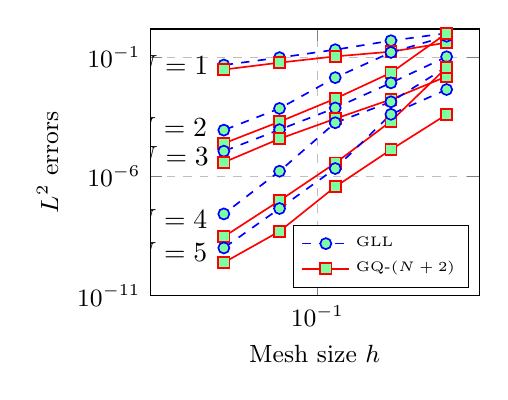
\begin{tikzpicture}
\begin{loglogaxis}[
    width=.475\textwidth,
    xlabel={Mesh size $h$},
    ylabel={$L^2$ errors}, 
    xmin=.0125, xmax=.75,
    ymin=1e-11, ymax=1.5,
    legend pos=south east, legend cell align=left, legend style={font=\tiny},	
    xmajorgrids=true, ymajorgrids=true, grid style=dashed,
    legend entries={GLL,GQ-$(N+2)$}    
]
\pgfplotsset{
cycle list={{blue, dashed, mark=*}, {red, mark=square*}}
}
%\addlegendimage{no markers,blue}
%\addlegendimage{no markers,red}

\addplot+[semithick, mark options={solid, fill=markercolor}]
% N = 1, tau = 0.000000 =======================
coordinates{(0.5,1)(0.25,0.485059)(0.125,0.203599)(0.0625,0.0947163)(0.03125,0.0463705)};
\addplot+[semithick, mark options={solid, fill=markercolor}]
%N = 1, tau = 0.000000 =======================
coordinates{(0.5,0.402314)(0.25,0.167917)(0.125,0.106574)(0.0625,0.058359)(0.03125,0.0298728)}
[yshift=2pt] node[left, pos=1.025, color=black] {$N = 1$};


\addplot+[semithick, mark options={solid, fill=markercolor}]
% N = 2, tau = 0.000000 =======================
coordinates{(0.5,0.746606)(0.25,0.156701)(0.125,0.0137392)(0.0625,0.000701926)(0.03125,8.64531e-05)};
\addplot+[semithick, mark options={solid, fill=markercolor}]
%N = 2, tau = 0.000000 =======================
coordinates{(0.5,0.993771)(0.25,0.0219437)(0.125,0.00180028)(0.0625,0.000194939)(0.03125,2.4045e-05)}
[yshift=7pt] node[left, pos=1.025, color=black] {$N = 2$};


\addplot+[semithick, mark options={solid, fill=markercolor}]
% N = 3, tau = 0.000000 =======================
coordinates{(0.5,0.103299)(0.25,0.00829887)(0.125,0.00073573)(0.0625,9.05975e-05)(0.03125,1.13596e-05)};
\addplot+[semithick, mark options={solid, fill=markercolor}]
%N = 3, tau = 0.000000 =======================
coordinates{(0.5,0.0154054)(0.25,0.00167426)(0.125,0.000260859)(0.0625,3.76182e-05)(0.03125,3.86238e-06)}
[yshift=3pt] node[left, pos=1.025, color=black] {$N = 3$};

\addplot+[semithick, mark options={solid, fill=markercolor}]
% N = 4, tau = 0.000000 =======================
coordinates{(0.5,0.0385542)(0.25,0.00133048)(0.125,0.000176663)(0.0625,1.64135e-06)(0.03125,2.66024e-08)};
\addplot+[semithick, mark options={solid, fill=markercolor}]
%N = 4, tau = 0.000000 =======================
coordinates{(0.5,0.0367592)(0.25,0.000202817)(0.125,3.57758e-06)(0.0625,9.58294e-08)(0.03125,2.94985e-09)}[yshift=8pt] node[left, pos=1.025, color=black] {$N = 4$};

\addplot+[semithick, mark options={solid, fill=markercolor}]
% N = 5, tau = 0.000000 =======================
coordinates{(0.5,0.00436131)(0.25,0.00039846)(0.125,2.1282e-06)(0.0625,4.49046e-08)(0.03125,9.99912e-10)};
\addplot+[semithick, mark options={solid, fill=markercolor}]
%N = 5, tau = 0.000000 =======================
coordinates{(0.5,0.000390565)(0.25,1.31188e-05)(0.125,3.6544e-07)(0.0625,4.95271e-09)(0.03125,2.42763e-10)}
[yshift=5pt] node[left, pos=1.025, color=black] {$N = 5$};

%\legend{$N=1$,$N=2$,$N=3$,$N=4$,$N=5$}
\end{loglogaxis}
\end{tikzpicture}
}
\subfloat[With Lax-Friedrichs penalization]{
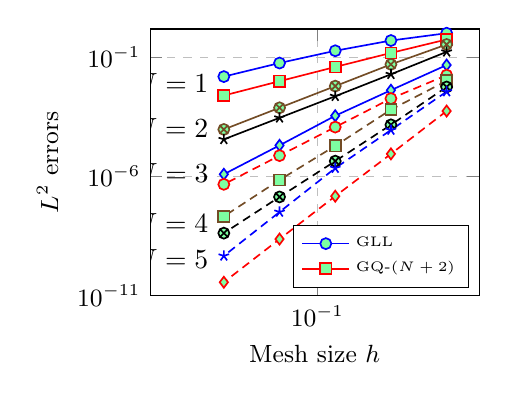
\begin{tikzpicture}
\begin{loglogaxis}[
    width=.475\textwidth,
    xlabel={Mesh size $h$},  ylabel={$L^2$ errors}, 
    xmin=.0125, xmax=.75,
    ymin=1e-11, ymax=1.5,
    legend pos=south east, legend cell align=left, legend style={font=\tiny},	
    xmajorgrids=true, ymajorgrids=true, grid style=dashed,
    legend entries={GLL,GQ-$(N+2)$}
] 
%\pgfplotsset{cycle list={{blue, dashed, mark=*}, {red, mark=square*}}}

\addplot+[semithick, mark options={solid, fill=markercolor}]
% N = 1, tau = 0.500000 =======================
coordinates{(0.5,1)(0.25,0.4932)(0.125,0.183839)(0.0625,0.0562398)(0.03125,0.0151873)};
\addplot+[semithick, mark options={solid, fill=markercolor}]
%N = 1, tau = 0.500000 =======================
coordinates{(0.5,0.547558)(0.25,0.148981)(0.125,0.0384647)(0.0625,0.00974763)(0.03125,0.00244539)}
[yshift=5pt] node[left, pos=1.025, color=black] {$N = 1$};

\addplot+[semithick, mark options={solid, fill=markercolor}]	
% N = 2, tau = 0.500000 =======================
coordinates{(0.5,0.336817)(0.25,0.04941)(0.125,0.00605428)(0.0625,0.000748842)(0.03125,9.25456e-05)};
\addplot+[semithick, mark options={solid, fill=markercolor}]
%N = 2, tau = 0.500000 =======================
coordinates{(0.5,0.165807)(0.25,0.0190013)(0.125,0.00227903)(0.0625,0.00028425)(0.03125,3.54865e-05)}
[yshift=5pt] node[left, pos=1.025, color=black] {$N = 2$};


% N = 3, tau = 0.500000 =======================
\addplot+[semithick, mark options={solid, fill=markercolor}]
coordinates{(0.5,0.0463242)(0.25,0.00408748)(0.125,0.000346831)(0.0625,1.99064e-05)(0.03125,1.22357e-06)};
\addplot+[semithick, mark options={solid, fill=markercolor}]
%N = 3, tau = 0.500000 =======================
coordinates{(0.5,0.0174194)(0.25,0.00182234)(0.125,0.000116147)(0.0625,7.39839e-06)(0.03125,4.6305e-07)}
[yshift=5pt] node[left, pos=1.025, color=black] {$N = 3$};

\addplot+[semithick, mark options={solid, fill=markercolor}]
% N = 4, tau = 0.500000 =======================
coordinates{(0.5,0.0100716)(0.25,0.000625923)(0.125,1.89866e-05)(0.0625,7.03865e-07)(0.03125,2.10265e-08)};
\addplot+[semithick, mark options={solid, fill=markercolor}]
%N = 4, tau = 0.500000 =======================
coordinates{(0.5,0.00556743)(0.25,0.000144595)(0.125,4.33972e-06)(0.0625,1.37151e-07)(0.03125,4.16335e-09)}
[yshift=5pt] node[left, pos=1.025, color=black] {$N = 4$};


\addplot+[semithick, mark options={solid, fill=markercolor}]
% N = 5, tau = 0.500000 =======================
coordinates{(0.5,0.00356628)(0.25,8.73125e-05)(0.125,2.20528e-06)(0.0625,3.20127e-08)(0.03125,4.63639e-10)};
\addplot+[semithick, mark options={solid, fill=markercolor}]
%N = 5, tau = 0.500000 =======================
coordinates{(0.5,0.000547621)(0.25,8.7194e-06)(0.125,1.47105e-07)(0.0625,2.34345e-09)(0.03125,3.65306e-11)}
[yshift=10pt] node[left, pos=1.025, color=black] {$N = 5$};

\end{loglogaxis}
\end{tikzpicture}
}
\caption{$L^2$ errors under mesh refinement for entropy conservative and Lax-Friedrichs fluxes under both Gauss-Legendre-Lobatto (GLL) and over-integrated $(N+2)$ point Gauss quadrature (GQ-$(N+2)$).}
\label{fig:convergence}
\end{figure}
We begin by verifying the high order accuracy of the proposed methods using a periodic entropy wave solution
\[
\rho(x,t) = 2 + \sin\LRp{\pi (x - t)}, \qquad u(x,t) = 1, \qquad p(x,t) = 1.
\]
We compute the $L^2$ error in the conservative variables 
\[
\nor{\bm{u} - \bm{u}_h}_{L^2}^2 = \nor{\rho - \rho_h}_{L^2}^2 + \nor{m - m_h}_{L^2}^2 + \nor{E - E_h}_{L^2}^2
\]
at final time $T = .7$ using both the entropy conservative and local Lax-Friedrichs fluxes and a CFL of .125.  For these experiments, we compare three quadrature rules: 
\begin{enumerate}
\item the $(N+1)$ point Gauss-Legendre-Lobatto rule (referred to as ``GLL''),
\item a $(N+1)$ point Gauss quadrature rule (referred to as ``GQ-$(N+1)$''),
\item an over-integrated $(N+2)$ point Gauss quadrature rule (referred to as ``GQ-$(N+2)$'').  
\end{enumerate}
The $L^2$ error is evaluated using a more accurate $N+5$ point Gauss quadrature rule.  

\begin{table}[h!]
\centering
 \begin{tabular}{||c | c |c |c |c | c|} 
 \hline
 &  $N=1$ &  $N=2$ &  $N=3$ &  $N=4$ &  $N=5$\\
 \hline
 GLL (entropy conservative) & 1.0672 & 3.6561  &  3.0086 &   6.3486 &   5.5278\\ 
 \hline
 GQ-$(N+2)$ (entropy conservative) &  0.9175  &  3.1132  &  3.0388 &   5.1221 &   5.2779 \\ 
 \hline
 GLL (Lax-Friedrichs) & 1.8887  &  3.0164  &  4.0241 &   5.0650 &   6.1095\\ 
 \hline
 GQ-$(N+2)$ (Lax-Friedrichs) & 1.9950  &  3.0018  &  3.9980  &  5.0419  &  6.0034\\ 
 \hline
 \end{tabular}
 \caption{Computed asymptotic convergence rates of $L^2$ errors under mesh refinement.}
 \label{tab:rates}
\end{table}

Figure~\ref{fig:convergence} shows computed $L^2$ errors under mesh refinement for both GLL and GQ-$(N+2)$ quadrature rules with and without Lax-Friedrichs penalization.  We do not compare against the $(N+1)$ point Gauss quadrature rule or quadrature rules with $N_q > (N+2)$, as the $L^2$ errors are very similar to the GQ-$(N+2)$ case.  Computed asymptotic convergence rates are reported in Table~\ref{tab:rates}.  It can be observed that, for both GLL and GQ-$(N+2)$ quadratures, the entropy conservative flux exhibits suboptimal convergence rates for odd orders, while the inclusion of Lax-Friedrichs penalization restores the optimal $O(h^{N+1})$ convergence rate for both quadrature choices.

\subsubsection{Discontinuous profile on a periodic domain}

Next, we examine the discrete evolution of entropy by evolving a discontinuous initial profile to final time $T=2$ on the domain $[-1,1]$.  We initialize the density and velocity to be 
\begin{equation}
\rho(x,t) = \begin{cases}
3 & \LRb{x} < 1/2\\
2 & \text{otherwise},
\end{cases} \qquad 
u(x,t) = 0, \qquad
p(x,t) = \rho^\gamma.
\label{eq:discontin}
\end{equation}
Periodic boundary conditions are enforced in order to examine the evolution of entropy over longer time periods.  Figure~\ref{subfig:sol} shows $\rho, u$ at time $T = 1/10$ using both entropy conservative and Lax-Friedrichs fluxes (referred to in the figure as ``EC'' and ``LF'', respectively) and GQ-$(N+2)$ quadrature.  As expected, the entropy conservative flux results in spurious high frequency oscillations, which are significantly damped under Lax-Friedrichs penalization.  

We next examine the change in entropy over time.  While the proof of conservation of entropy holds at the semi-discrete level, it does not take into account the time discretization and thus does not hold at the fully discrete level.  This is reflected in the observation that the numerical change in entropy 
\[
\Delta U(t) = U\LRp{\bm{u}(x,t)} - U\LRp{\bm{u}(x,0)}
\]
increases as $t$ increases.  However, numerical experiments in \cite{gassner2016well} suggest that the discrete change in entropy over time should converge to zero as the timestep decreases.%, which (under appropriate assumptions) implies that the fully discrete scheme converges to the semi-discrete scheme.  

Figure~\ref{subfig:dS} shows the evolution of $\Delta U(t)$ to final time $T=2$ for both entropy conservative and Lax-Friedrichs fluxes at various CFL numbers.  For the entropy conservative flux, we observe that $\Delta U(t)$ decreases as the CFL and timestep $\Delta t$ decrease.  This is expected, since the discrete time problem should converge to the continuous semi-discrete problem (for which $\Delta U(t) = 0$) as $\Delta t\rightarrow 0$.  We also observe that $\Delta U(t)$ does not change significantly as a function of the CFL for the Lax-Friedrichs flux, indicating that the non-zero change in entropy in this case is due to the effect of the dissipative flux rather than the time discretization.

\begin{figure}
\centering
\subfloat[Solution at time $T = .1$]{
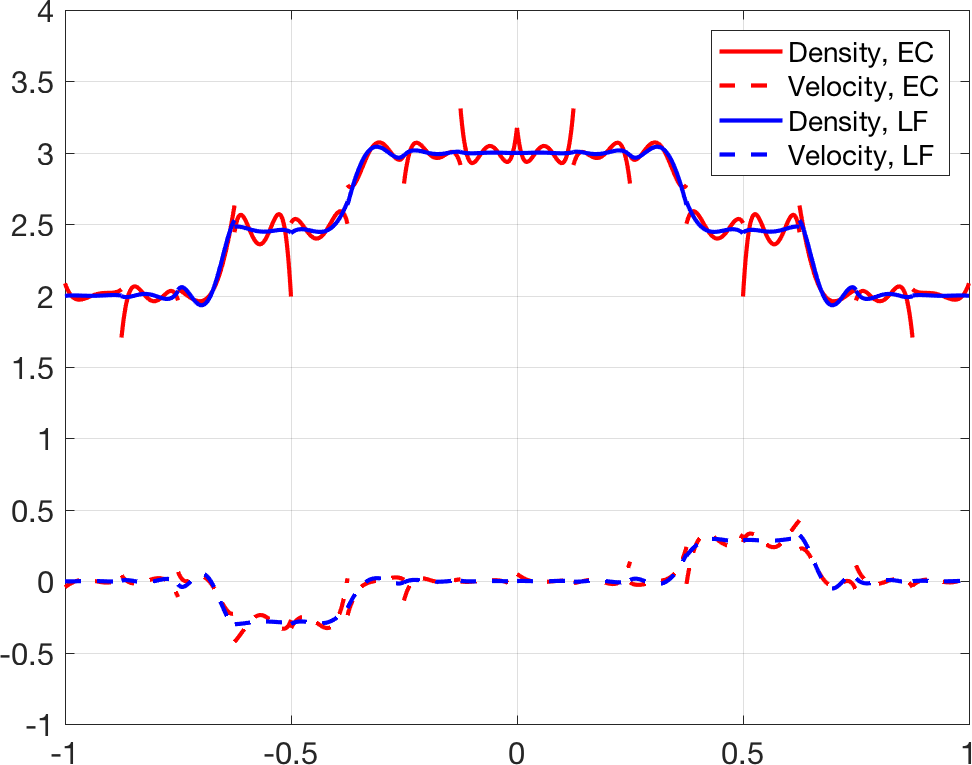
\includegraphics[width=.475\textwidth]{sol_ECLF.png}
\label{subfig:sol}}
\hspace{.5em}
\subfloat[$\Delta U(t)$]{
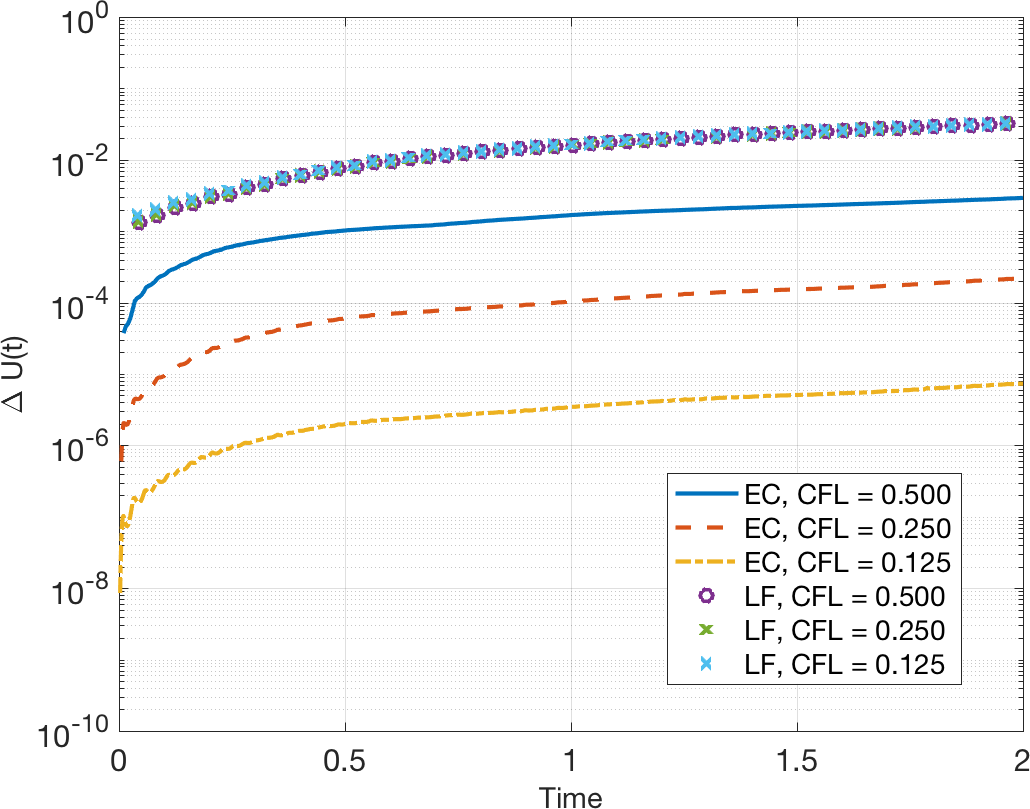
\includegraphics[width=.475\textwidth]{dS_ECLF.png}
\label{subfig:dS}}
\caption{Solution snapshot and change in entropy $\Delta U(t)$ for both entropy conservative (EC) and Lax-Friedrichs (LF) fluxes.}
\label{fig:dS}
\end{figure}

We also numerically evaluate the spatial formulation tested against the projected entropy variables
\[
\delta(t) = \LRb{\LRp{\left.\LRp{D^x_h \bm{f}_S(\bm{u}_{\bm{v}}(x),\bm{u}_{\bm{v}}(y))}\right|_{y=x},\Pi_N \bm{v}}_{\Omega}}, \qquad  \qquad 0\leq t \leq T.
\]
We utilize the non-dissipative entropy conservative flux and evolve the initial profile (\ref{eq:discontin}) until time $T = 1$ using a GQ-$(N+2)$ quadrature rule.  From Theorem~\ref{thm:ecdg_global}, we expect $\delta_{\max} = \max_{t\in (0,T)}{\delta}$ to be machine zero.  In practice, we have found that $\delta_{\max}$ depends on the tolerance $\epsilon$ used in evaluation of the logarithmic mean.  For a simulation to time $T=4$ using $N=4$ and $K = 16$ with a CFL of $1/2$, we observe that using $\epsilon = 10^{-2}$ (as recommended in \cite{ismail2009affordable}) results in $\delta_{\max} = O\LRp{10^{-10}}$.  Decreasing $\epsilon$ to $10^{-3}$ reduces $\delta_{\max}$ to $O\LRp{10^{-14}}$, and decreasing $\epsilon$ further to $1\times 10^{-4}$ reduces $\delta_{\max}$ to $10^{-15}$.  Smaller values of $\epsilon$ do result in observable changes to $\delta_{\max}$, and we do not observe any significant dependence of $\delta_{\max}$ on other discretization parameters.  

\begin{figure}
\centering
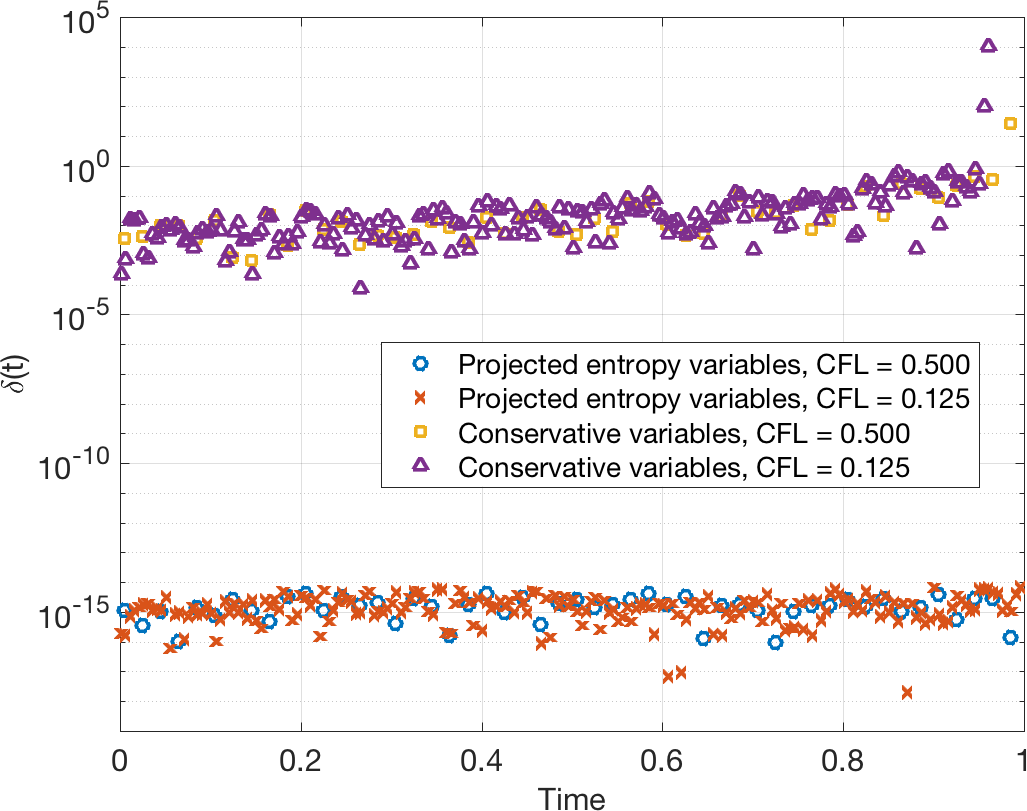
\includegraphics[width=.525\textwidth]{rhstest.png}
\caption{Comparison of $\delta(t)$ when evaluating the flux function $\bm{f}_S$ using conservative variables and projected entropy variables.}
\label{fig:rhstest}
\end{figure}
Next, in order to illustrate the importance of evaluating the flux in terms of the projected entropy variables $\Pi_N \bm{v}$, we compute $\delta(t)$ while evaluating the flux function $\bm{f}_S$ directly in terms of the conservative variables $\bm{u}(x)$ and in terms of the projected entropy variables $\bm{u}\LRp{(\Pi_N \bm{v})(x)}$.  It can be observed from Figure~\ref{fig:rhstest} that $\delta(t)$ is near machine precision when evaluating the flux in terms of the projected entropy variables.  When evaluating the flux function directly in terms of the conservative variables, $\delta(t)$ begins near $10^{-4}$ but grows steadily, blowing up exponentially near $t = 1$.  

\subsubsection{Sod shock tube}

We now examine the behavior of the proposed DG methods for some common one-dimensional test problems.  We begin with the Sod shock tube, which is posed on the domain $[-1/2,1/2]$ with initial conditions
\[
\rho = \begin{cases}
1 & x < 0\\
.125 & x \geq 0,
\end{cases} 
\qquad
u = 0, \qquad
p = \begin{cases}
1 & x < 0\\
.1 & x \geq 0.
\end{cases}
\]
Boundary conditions are enforced by taking the external value $\bm{u}^+$ in the numerical flux to be that of the initial condition at $x = \pm 1$.  The solution develops a left-moving rarefaction, as well as a right moving shock wave and a contact discontinuity.  We simulate the solution until time $T = .2$, without the use of positivity preserving or TVD-type limiters.  For all choices of quadrature tested, the solution diverges when using the entropy conservative flux, which is a result of oscillations in the solution and density and temperature becoming negative.  This is remedied when using the dissipative Lax-Friedrichs flux, for which we do not observe blowup of the solution.  
\begin{figure}
\centering
\subfloat[GLL quadrature]{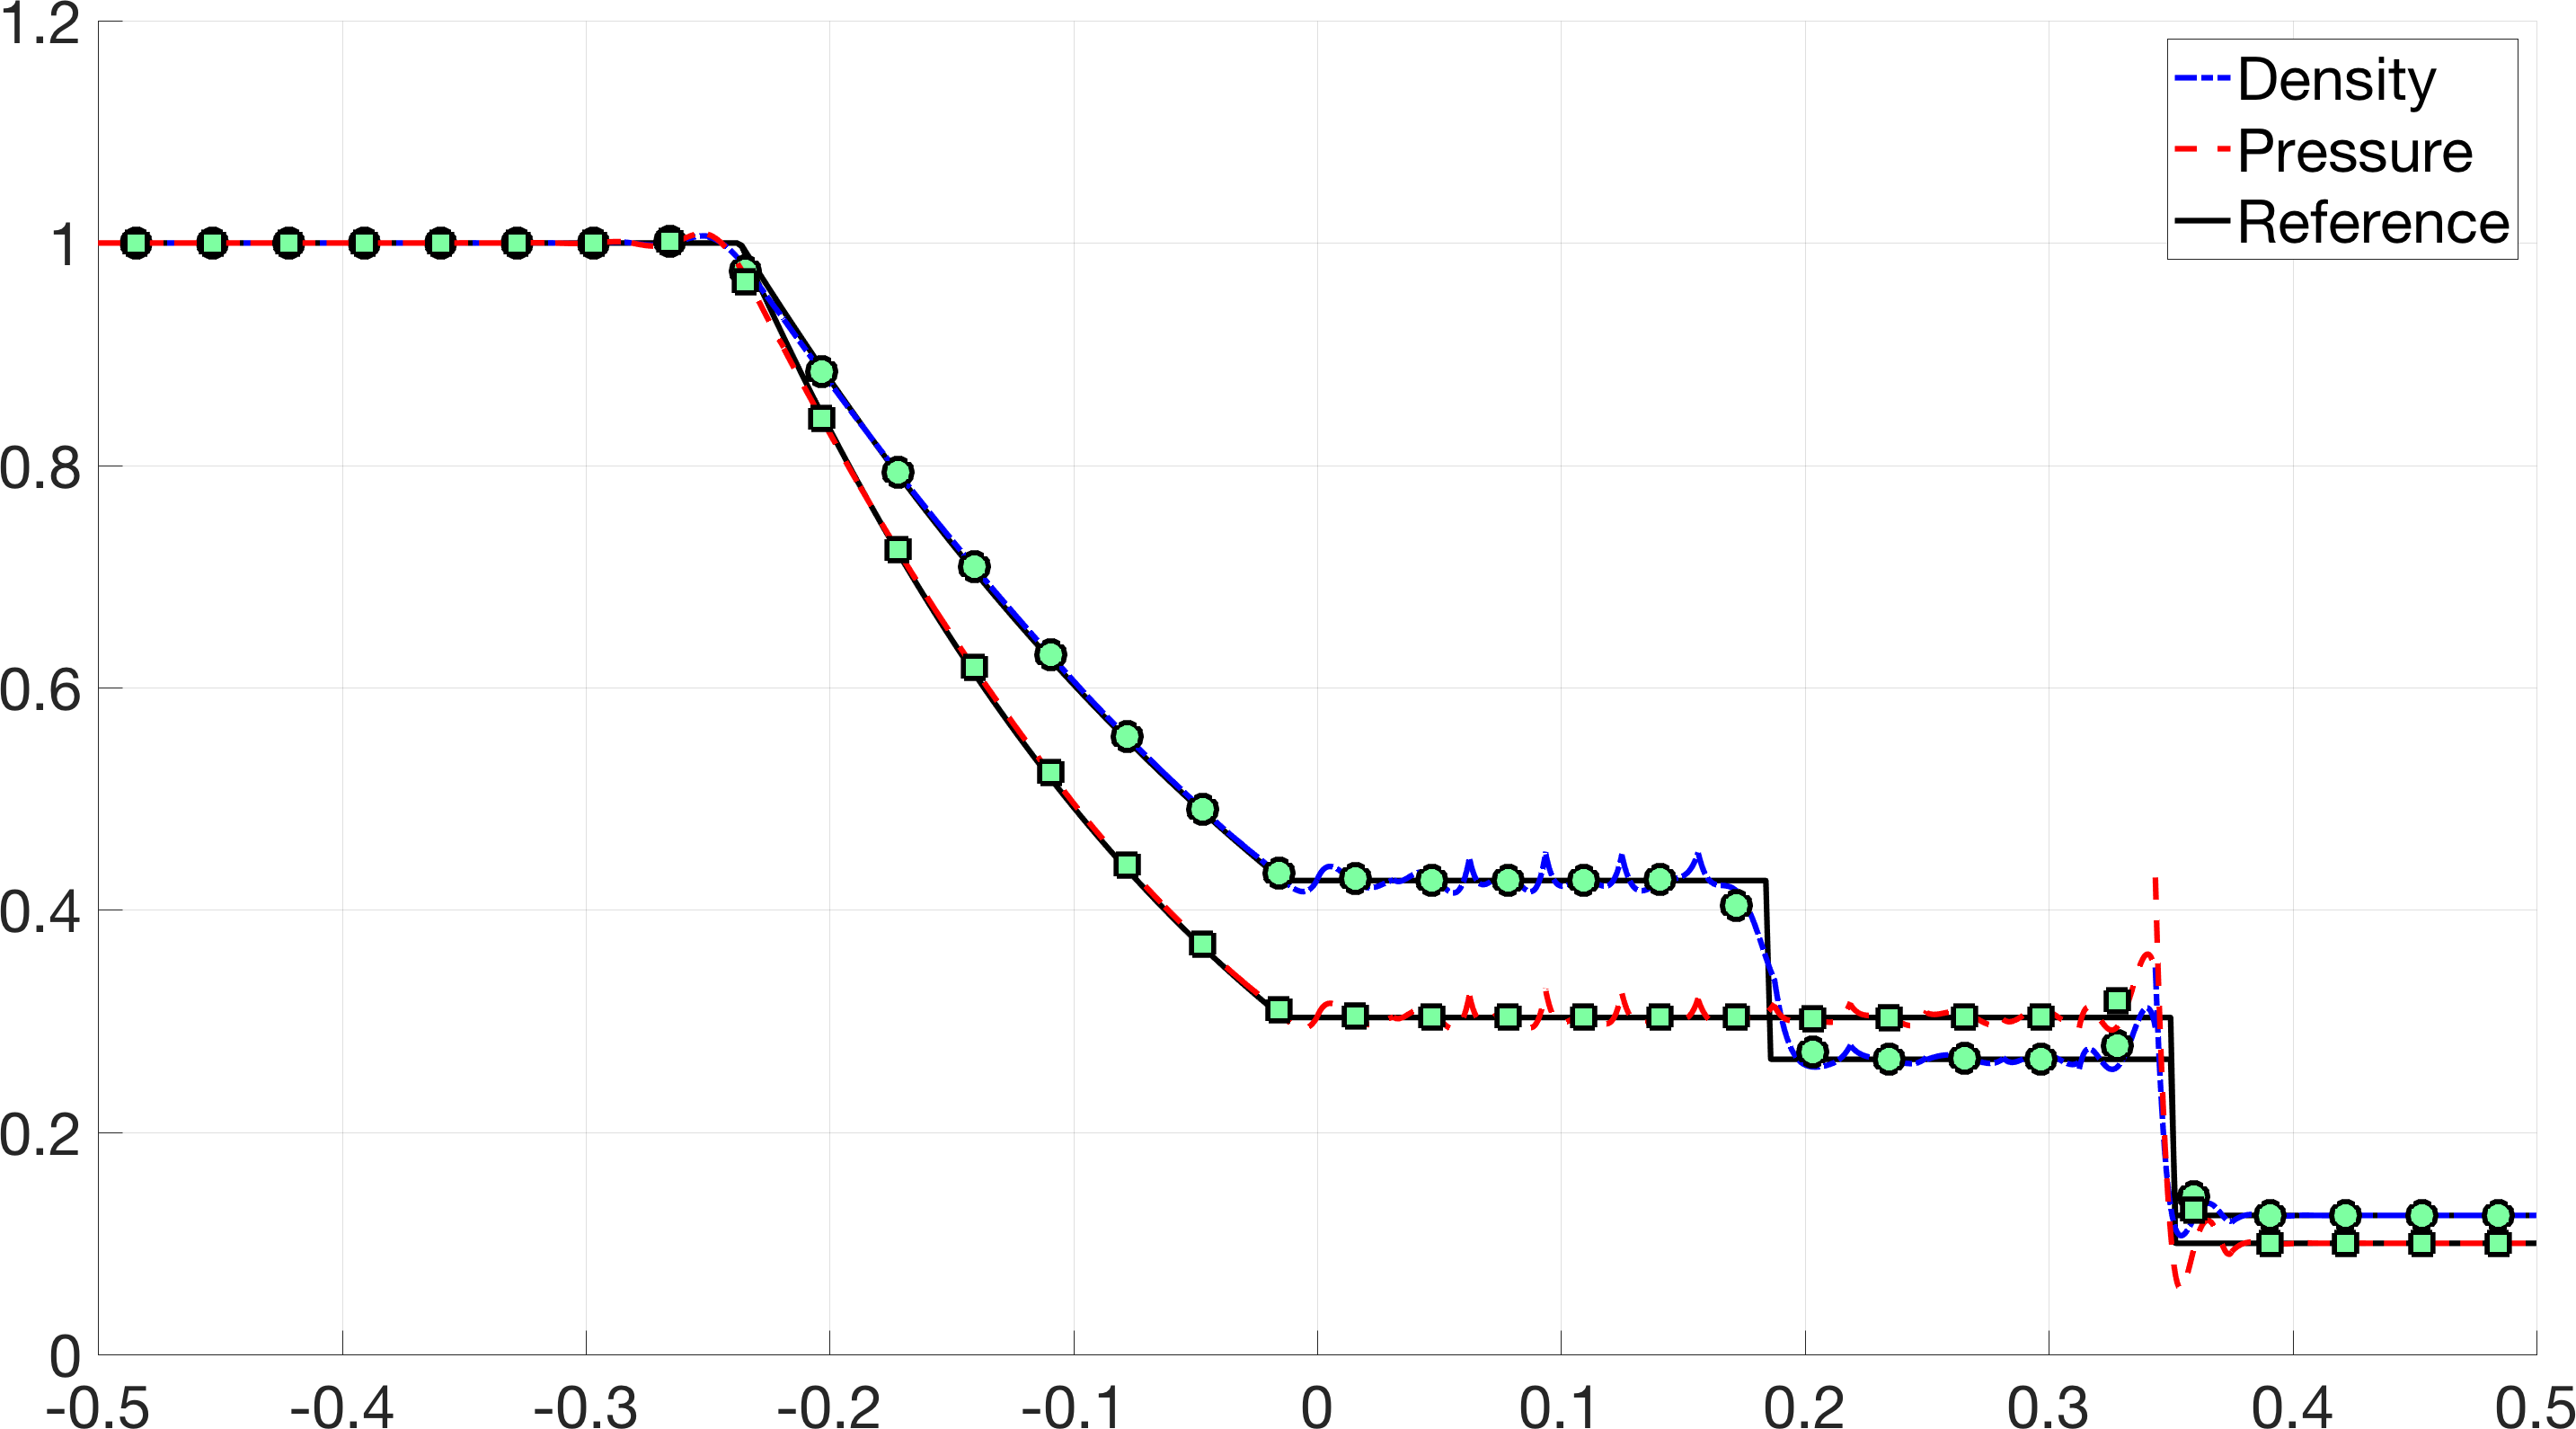
\includegraphics[width=.475\textwidth]{sodGLL.png}}
\hspace{.1em}
\subfloat[GQ-$(N+2)$ quadrature]{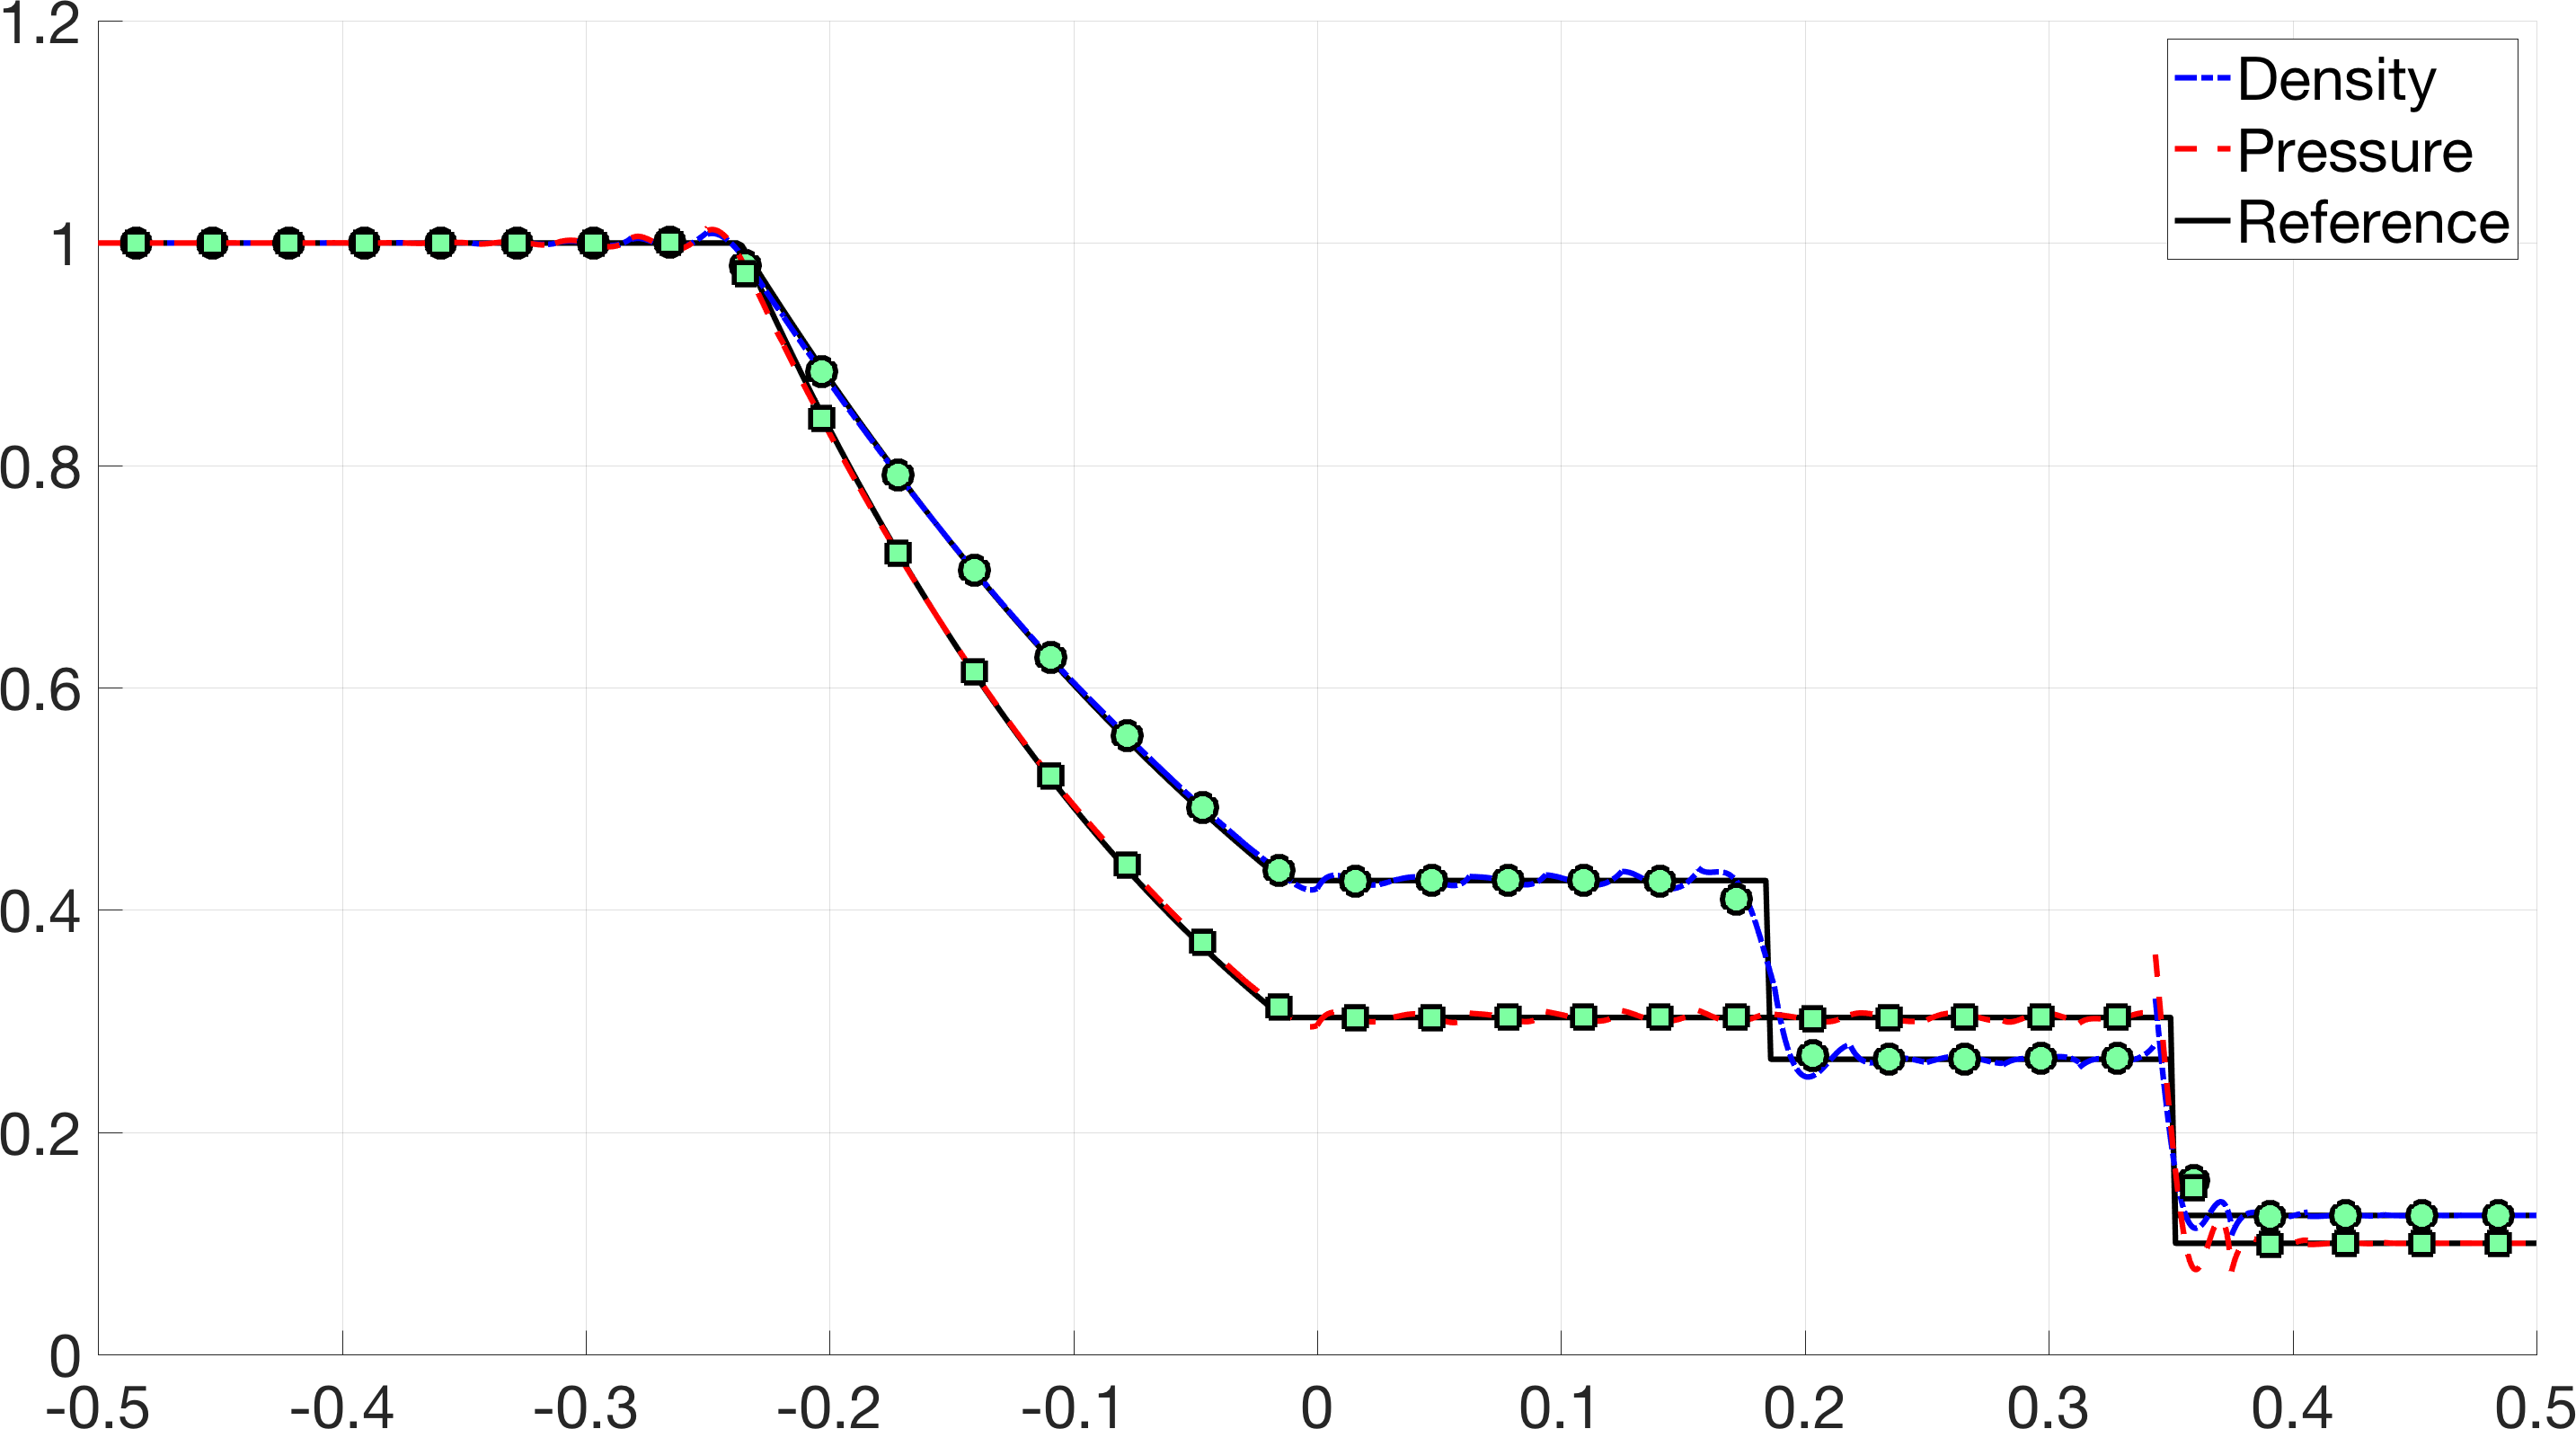
\includegraphics[width=.475\textwidth]{sodGQ2.png}}
\caption{Density and pressure solutions for the Sod shock tube at $T = .2$ for $N = 4$ and $K = 32$ elements.  Cell averages are overlaid as filled circles.  }
\label{fig:sod}
\end{figure}

Figure~\ref{fig:sod} shows both the exact solution and the computed density and pressure along with their cell averages.  These results were obtained using a CFL of $.125$ and GLL and GQ-$(N+2)$ quadrature rules.  For both quadratures, the cell averages agree relatively well with the exact solution.  Both solutions contain spurious oscillations, though the oscillations under GQ-$(N+2)$ quadrature appear qualitatively smoother and smaller.  

%\note{Add discussion of Figure~\ref{fig:sod} - reference solution is exact solution computed using a Riemann solver (``PRINCIPLES OF COMPUTATIONAL FLUID DYNAMICS'' by P. Wesseling).  }

\subsubsection{Sine-shock interaction}
\label{sec:sineshock}

The next benchmark problem we consider is the sine-shock interaction problem, which is posed on domain $[-5,5]$ with initial conditions
\[
\rho(x,0) = \begin{cases}
3.857143 & x < -4\\
1 + .2\sin(5x) & x \geq -4,
\end{cases} 
\qquad
u(x,0) = \begin{cases}
2.629369 & x < -4\\
0 & x \geq -4,
\end{cases}
\qquad
p(x,0) = \begin{cases}
10.3333 & x < -4\\
1 & x \geq -4.
\end{cases}
\]
We simulate the solution using different quadrature rules with $N=4$, $K=40$ elements, and a Lax-Friedrichs flux.  No TVD or positivity-preserving limiters are applied.  A smaller CFL of $.05$ is used, and is necessary to avoid solution divergence when using GQ-$(N+2)$ quadrature.  It should be pointed out that, for GLL quadrature, it is possible to use a larger CFL of $.125$ without observing solution blowup.  The reason for this discrepancy is the sensitivity of the evaluation $\bm{u}\LRp{\Pi_N \bm{v}}$ when $\Pi_N \bm{v}$ differs significantly from $\bm{v}$, and is described in more detail in Section~\ref{sec:instab}.  
\begin{figure}
\centering
%\subfloat[GLL quadrature]{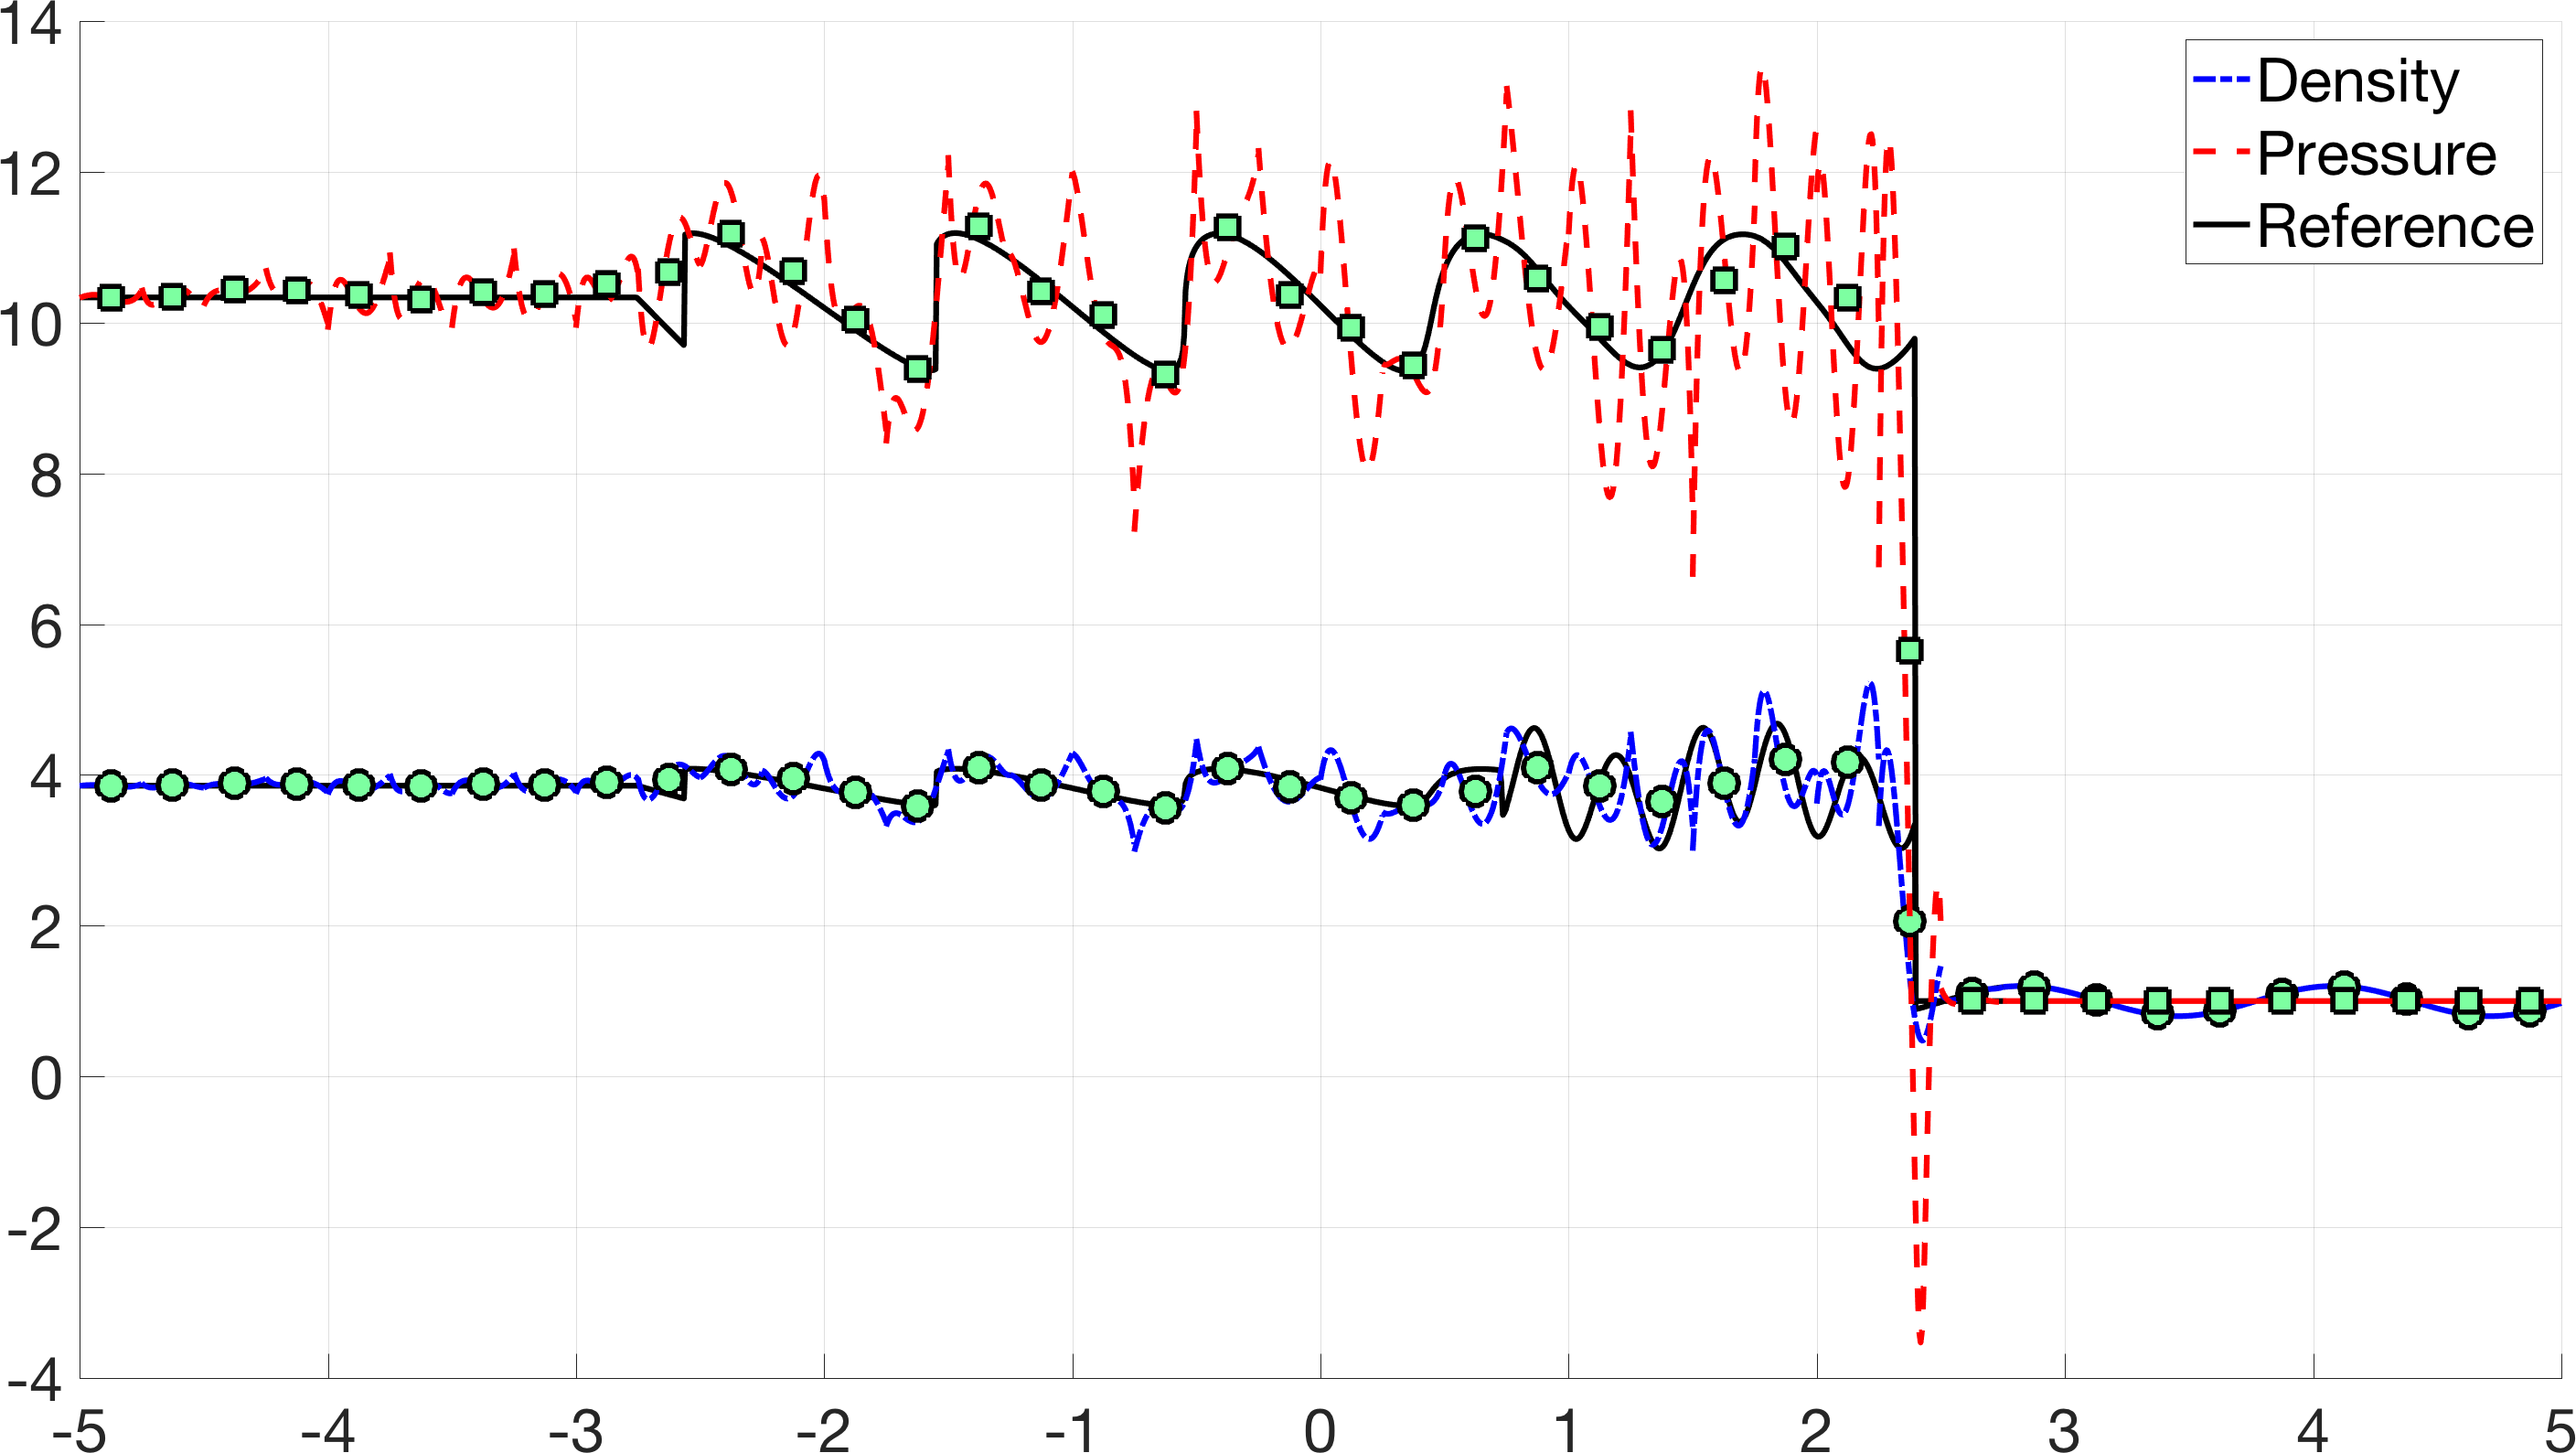
\includegraphics[width=.475\textwidth]{sineShockGLLrhop.png}}
\subfloat[GLL quadrature]{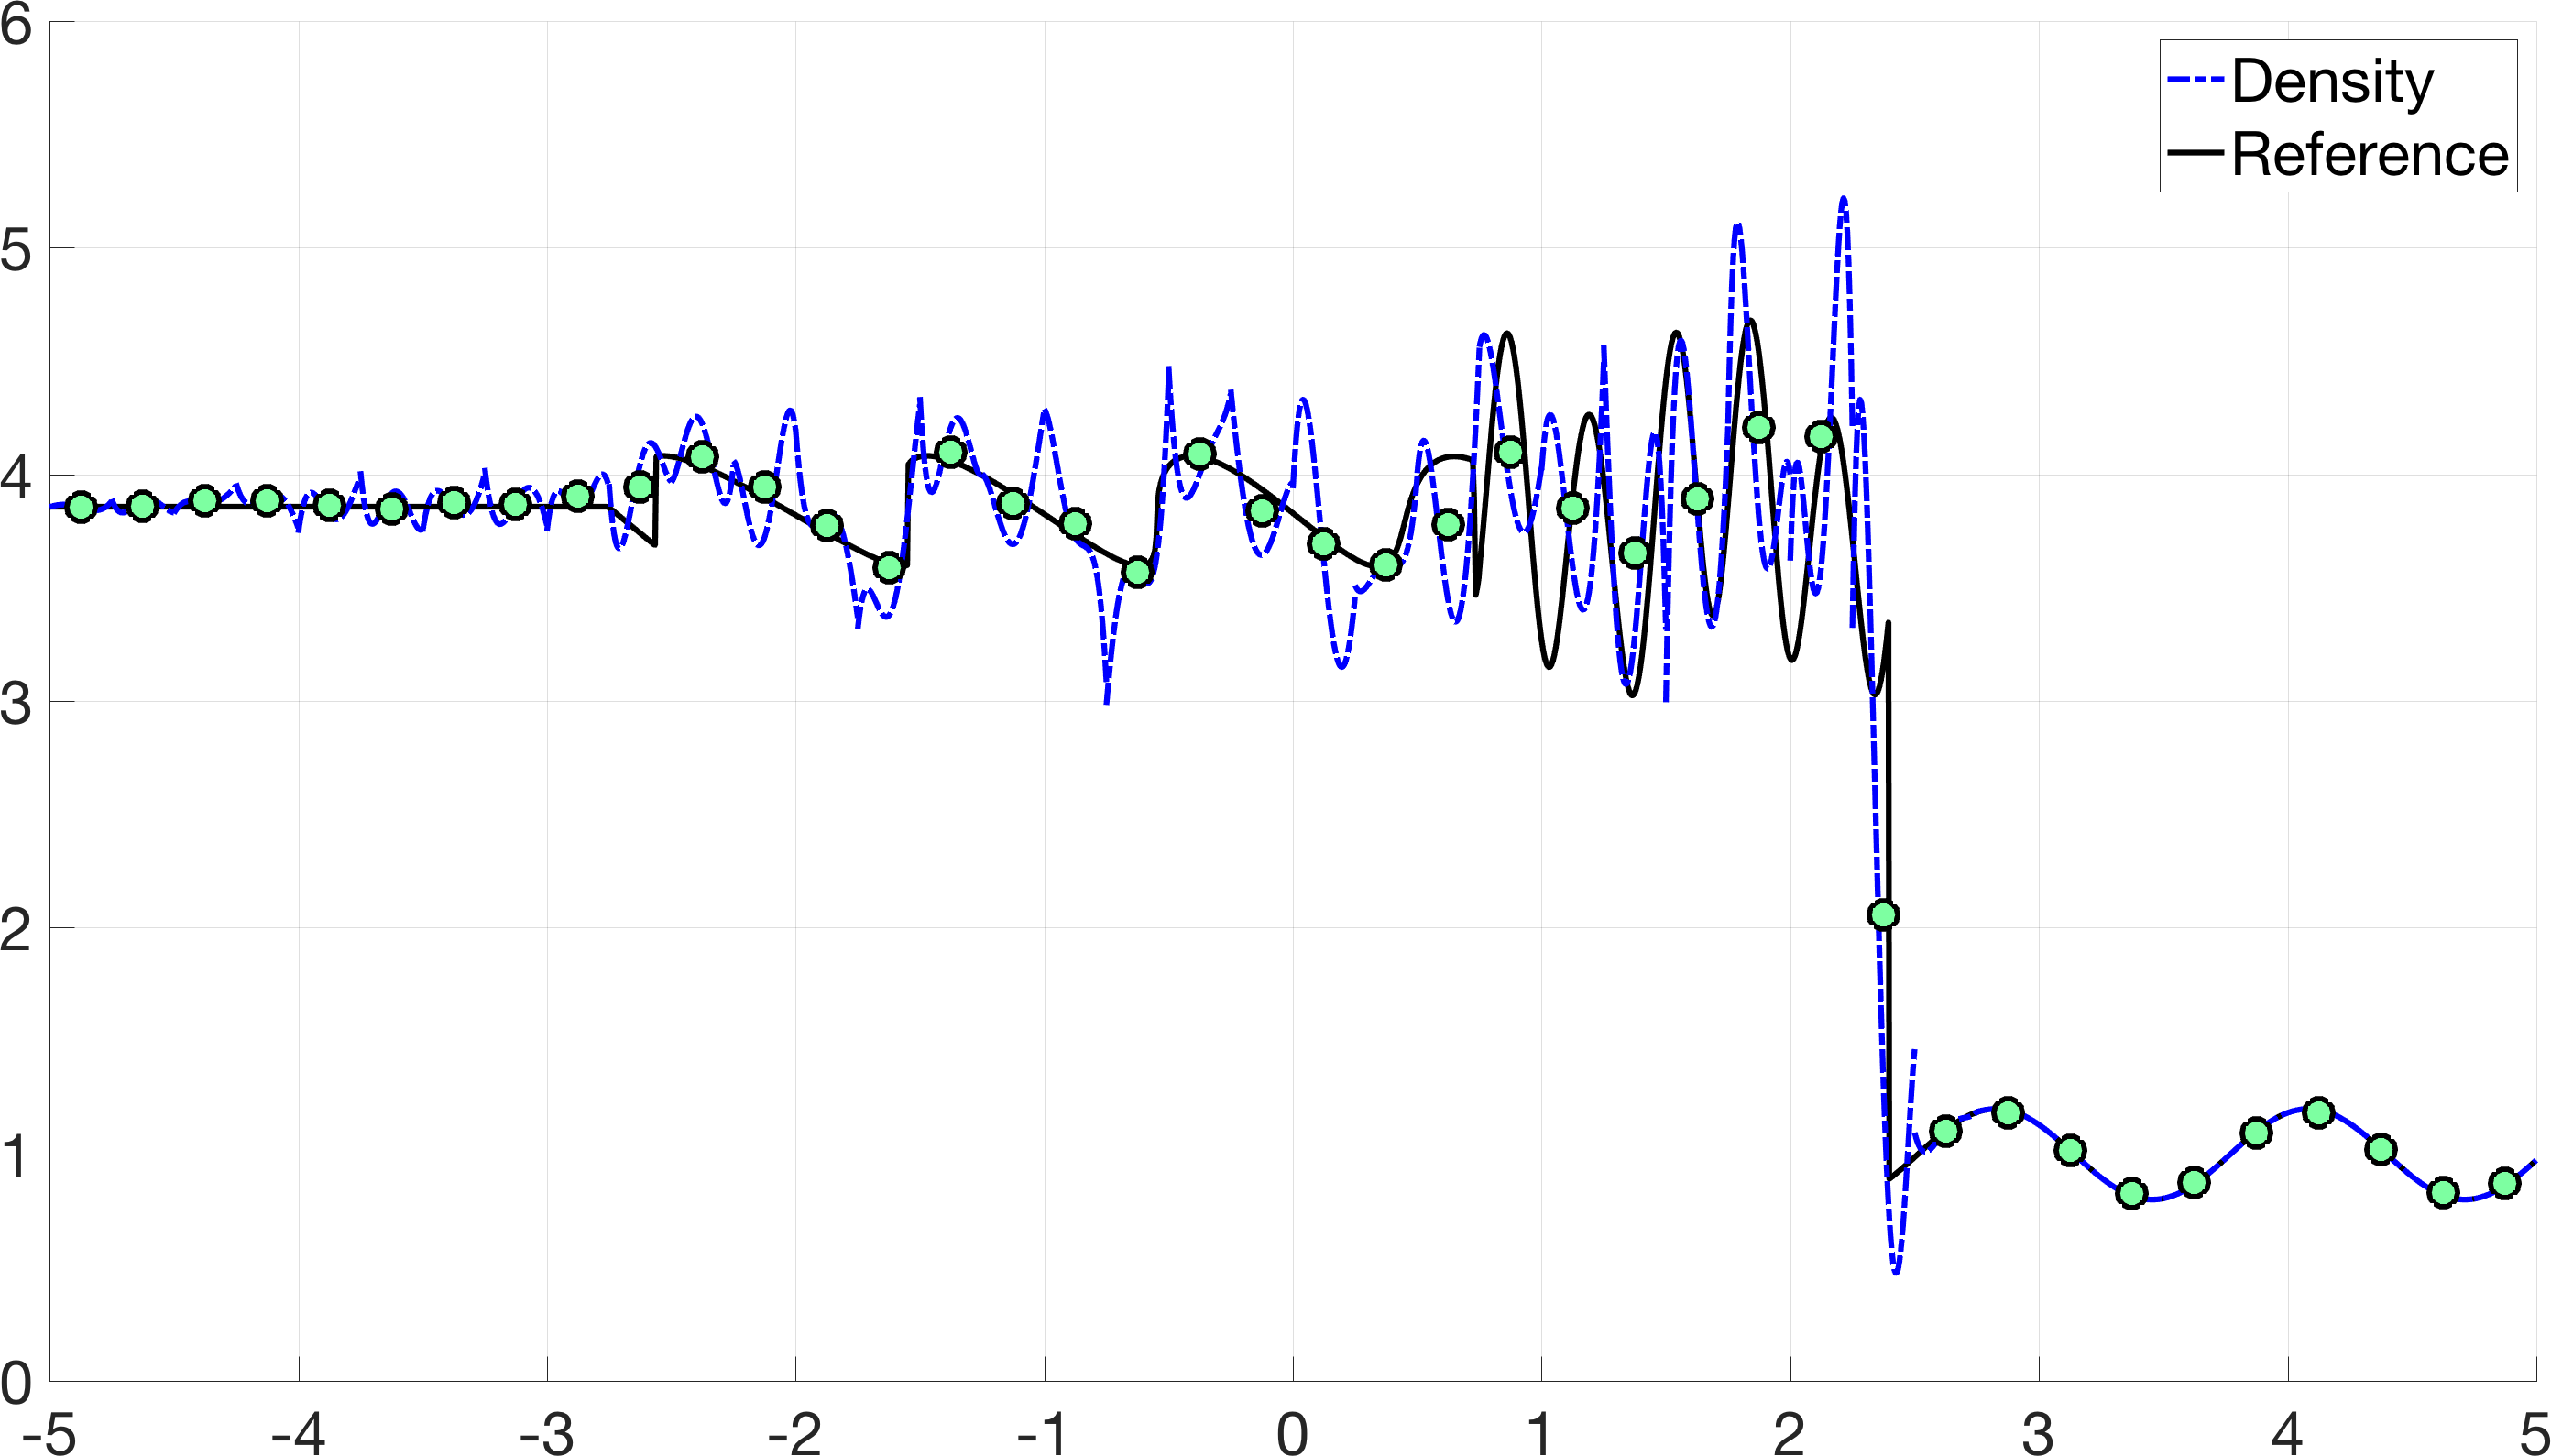
\includegraphics[width=.475\textwidth]{sineShockGLL.png}}
\hspace{.1em}
%\subfloat[GQ-$(N+2)$ quadrature]{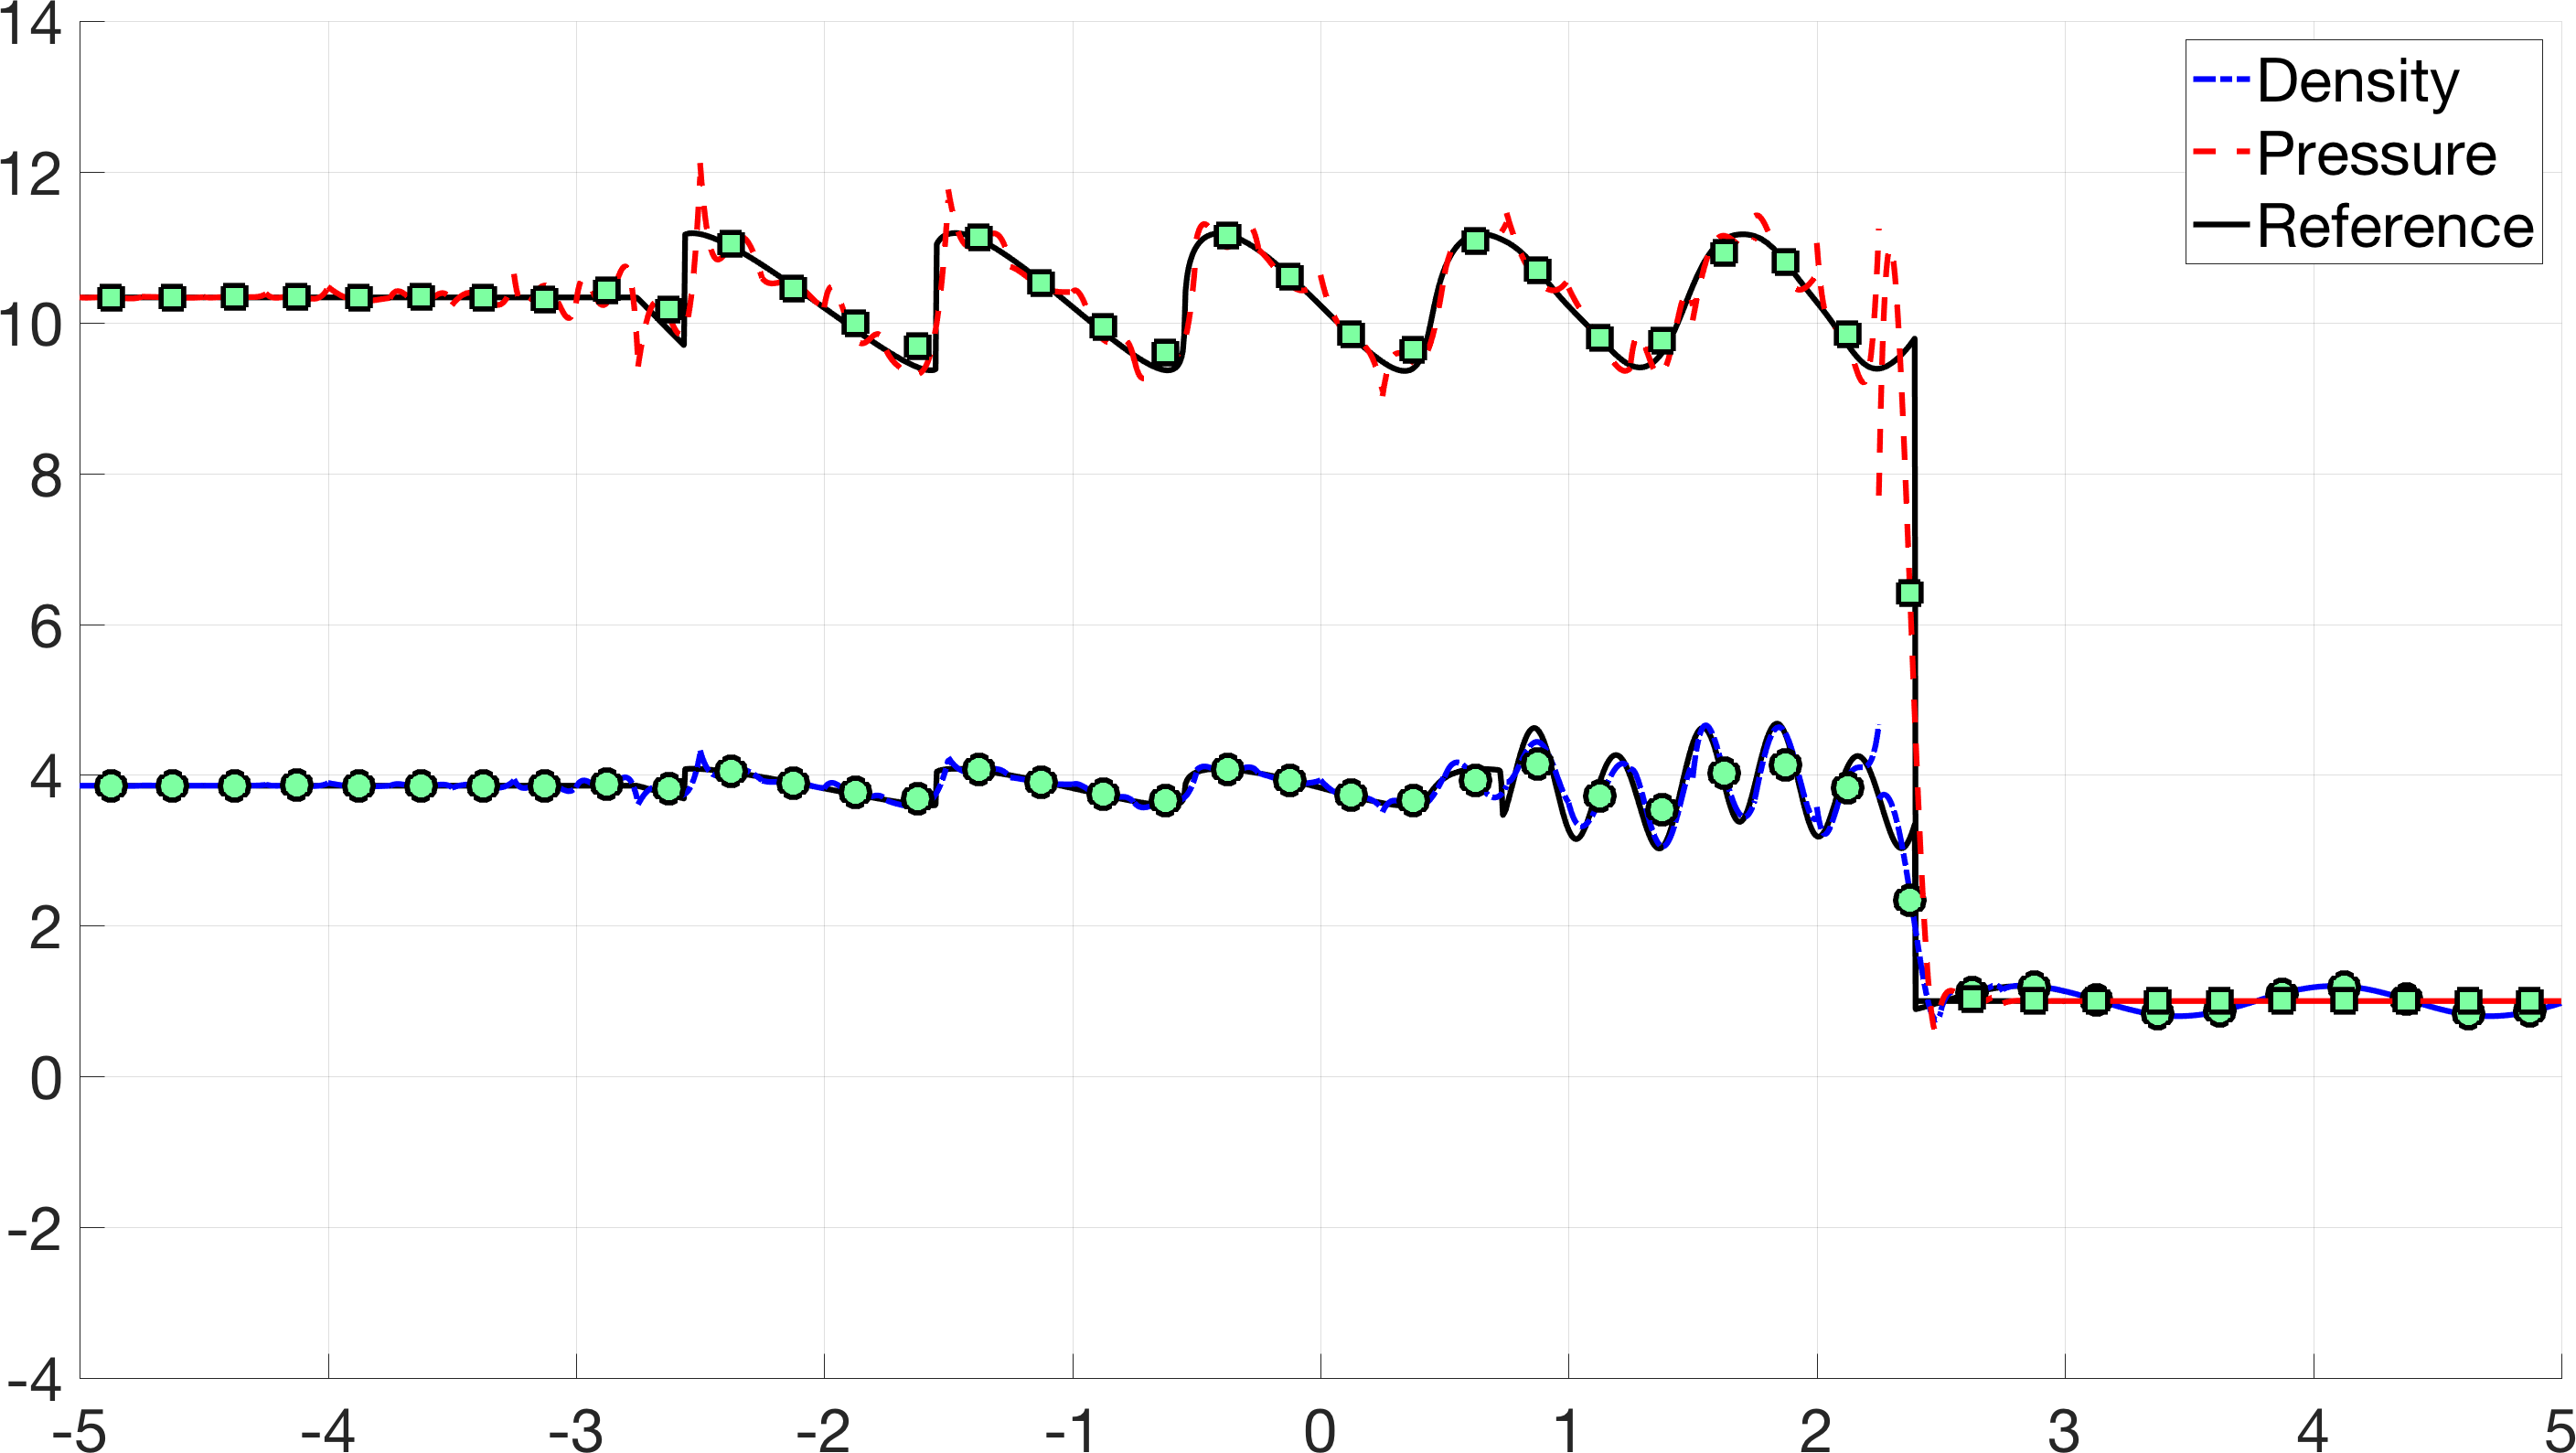
\includegraphics[width=.475\textwidth]{sineShockGQ2rhop.png}}
\subfloat[GQ-$(N+2)$ quadrature]{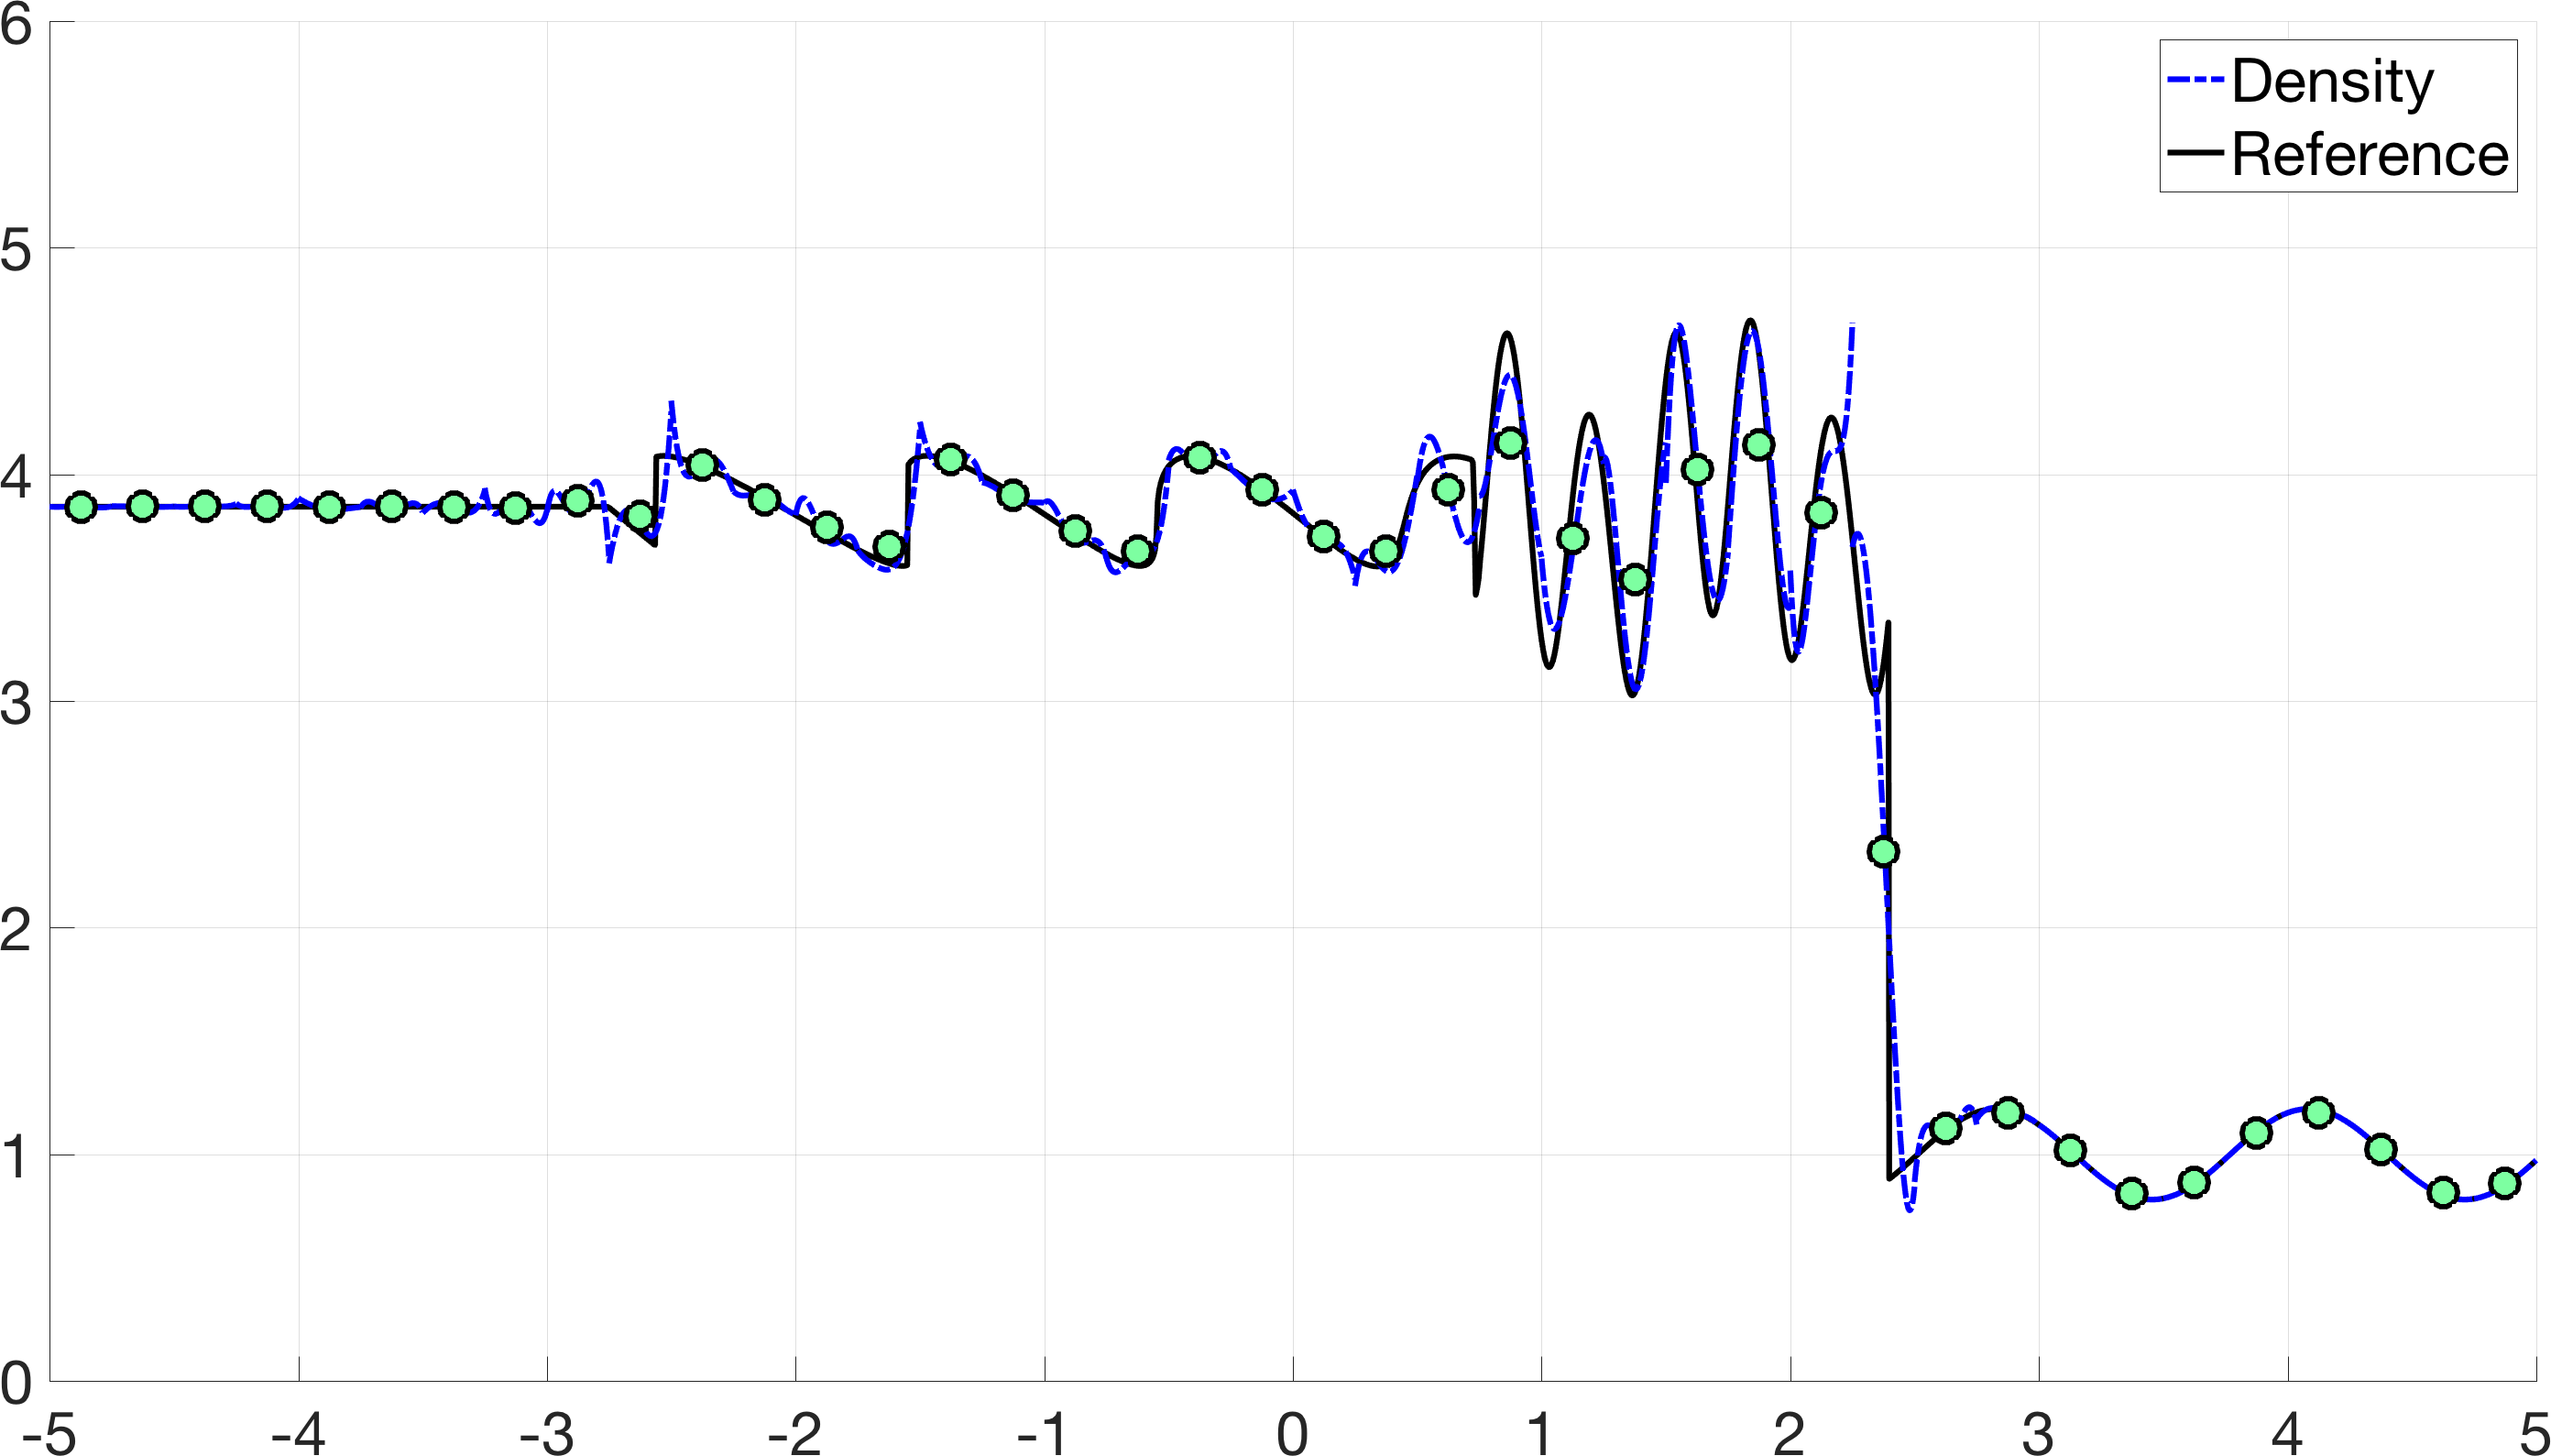
\includegraphics[width=.475\textwidth]{sineShockGQ2.png}}
\caption{Density solutions for the sine-shock interaction problem at $T = 1.8$ for $N = 4$ and $K = 40$ elements.  Cell averages are overlaid as filled circles.  }
\label{fig:sineshock}
\end{figure}

Figure~\ref{fig:sineshock} shows snapshots of the density at final time $T= 1.8$ for both GLL and GQ-$(N+2)$ quadrature, along with a reference solution computed using a 5th order WENO scheme with 25000 cells \cite{shu2009high}.  For both GLL and GQ-$(N+2)$ quadrature, the cell averages are close to the reference solution, though the solutions still contain spurious oscillations resulting from the presence of shocks and discontinuities.  However, as with the Sod shock tube, we observe that these oscillations are smoother and smaller in amplitude for the choice of GQ-$(N+2)$ quadrature.  

%\note{Add reference solution using 25000 cell 5th order WENO method \cite{shu2009high}.  Simulations in Figure~\ref{fig:sineshock} use CFL of $.05$; necessary for GQ-$(N+2)$.  GLL can still run at CFL of $.125$.  }

\subsubsection{Sensitivity of evaluation in terms of the projected entropy variables}
\label{sec:instab}

The numerical experiments in previous sections suggest that solutions computed using Gauss quadrature rules can be more accurate than those computed using GLL quadratures.  However, we also observe that, for the sine-shock interaction problem, a larger CFL of $.125$ can be taken when using GLL quadrature, whereas a much smaller CFL of $.05$ is required to prevent solution blowup when using GQ-$(N+1)$ and GQ-$(N+2)$ quadratures.  %The reason for this discrepancy between Gauss-Lobatto and Gauss quadratures is the presence of boundary nodes in GLL quadratures.  
For GQ-$(N+1)$ and GQ-$(N+2)$ quadratures, solution spikes can occur when evaluating the conservative variables in terms of the projected entropy variables at surface points.  The use of GLL quadrature avoids this phenomena because of two factors: the equivalence between interpolation and projection under a $(N+1)$ point quadrature rule, and the presence of boundary points in GLL quadrature.  

Figure~\ref{fig:proj} shows snapshots of different variables for $N=2$ and $K = 20$ elements at the fifth Runge-Kutta stage of the first timestep (just prior to the detection of negative density and pressure values) using a GQ-$(N+2)$ quadrature rule.  Discrepancies between the evaluated and projected values of the entropy variables $v_1, v_2, v_3$ at element boundaries are present, and while these discrepancies are not extremely large, they produce large spikes in the conservative variables due to the sensitivity of the nonlinear evaluation $\bm{u}\LRp{\Pi_N \bm{v}}$.  In particular, because $v_3$ appears in the denominators of entropy and $\rho e$ (as functions of the entropy variables), values of $v_3$ near zero result in large values of density and energy.  These spikes result in large oscillations in the solution if the CFL is too large, which eventually cause the density and pressure to become negative at quadrature or boundary points.  %\footnote{For the sine-shock interaction problem, these spikes appear to be related to the large jump in the pressure initial condition.  Instabilities were not observed for the sine-shock interaction when using an initial pressure condition with a smaller magnitude jump, or for other problems with discontinuous non-zero initial profiles, such as the modified Sod problem \cite{ranocha2017comparison}. }
\begin{figure}
\centering
\subfloat[$v_1$ and $\Pi_N(v_1)$]{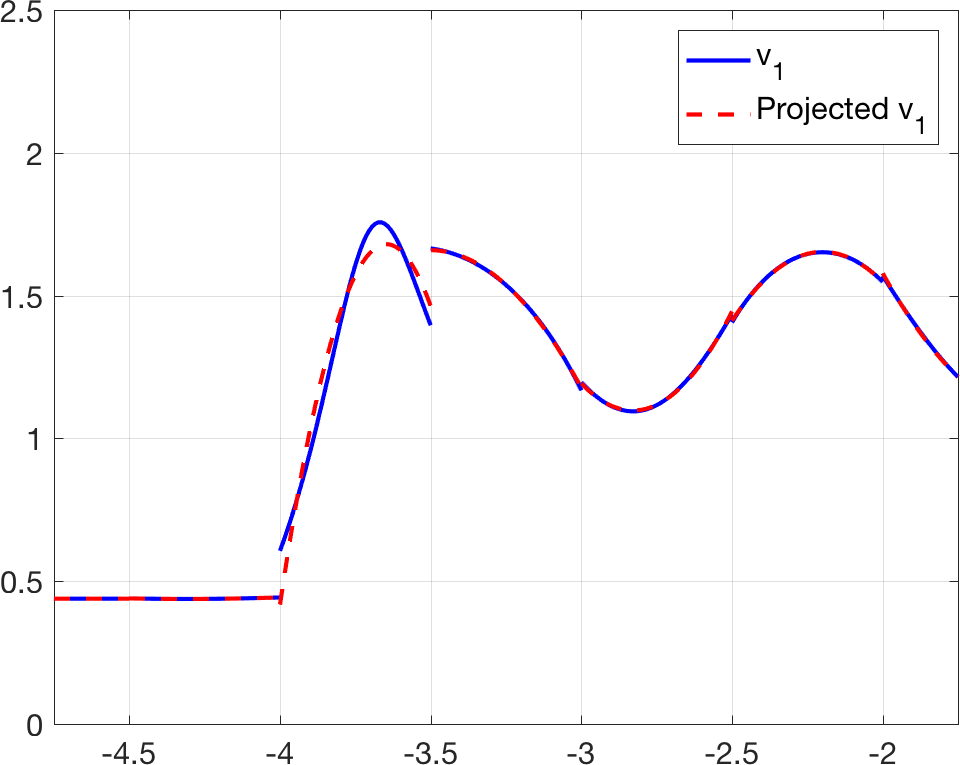
\includegraphics[width=.32\textwidth]{sineShockQ1Compare.png}}\label{subfig:v1}
\hspace{.1em}
\subfloat[$v_2$ and $\Pi_N(v_2)$]{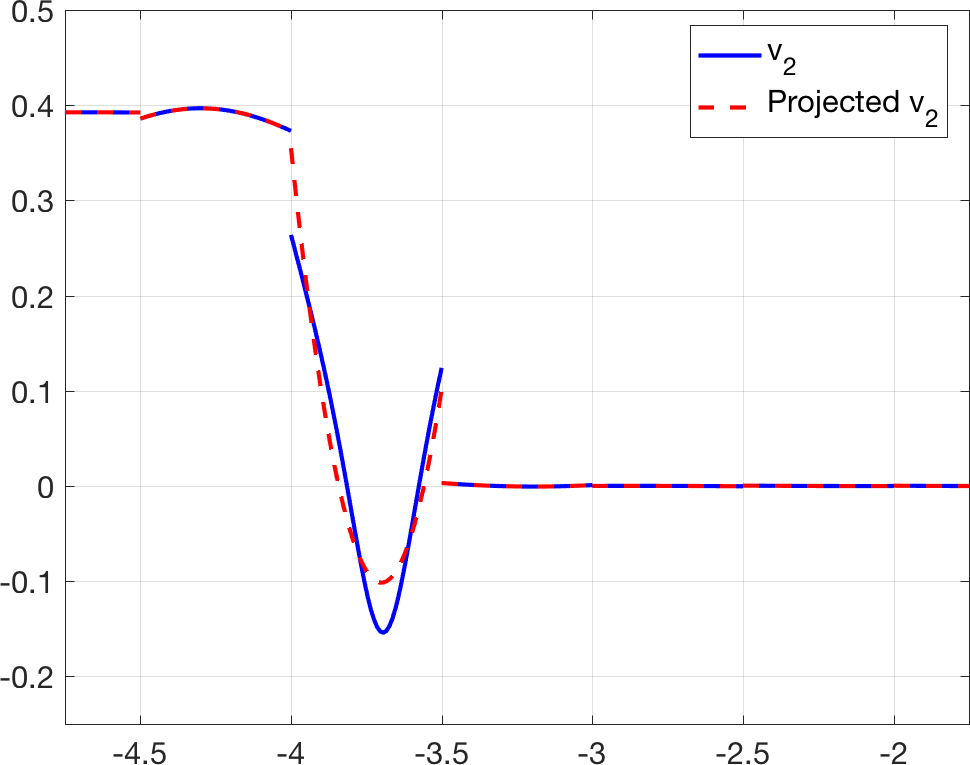
\includegraphics[width=.32\textwidth]{sineShockQ2Compare.png}}\label{subfig:v2}
\hspace{.1em}
\subfloat[$v_3$ and $\Pi_N(v_3)$]{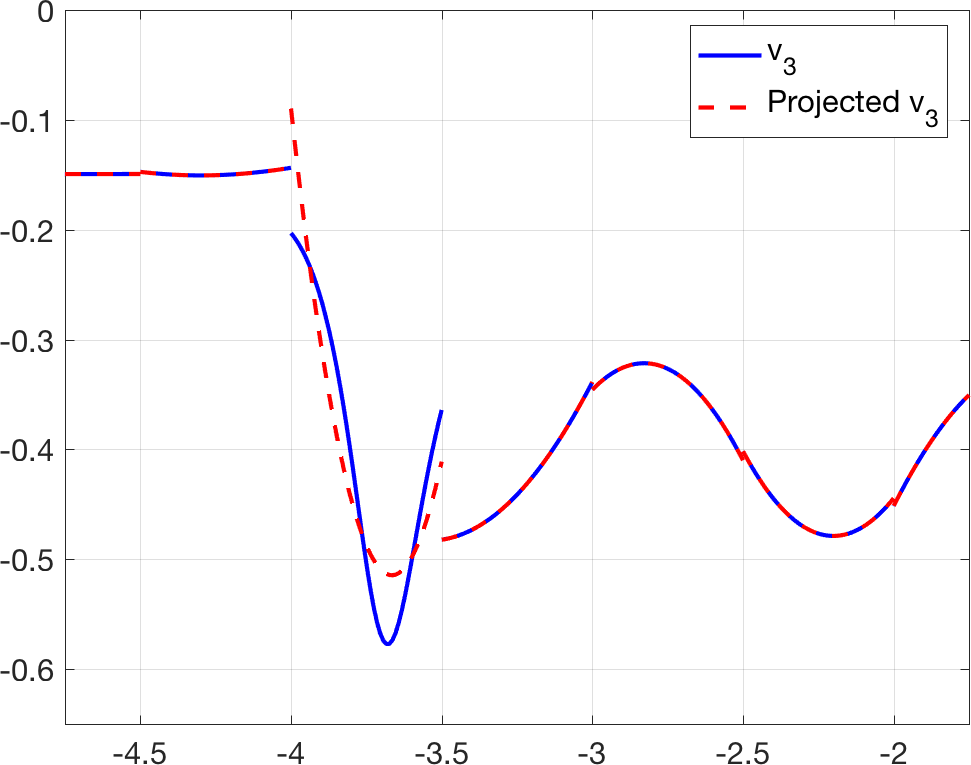
\includegraphics[width=.32\textwidth]{sineShockQ3Compare.png}}\label{subfig:v3}\\
\subfloat[$\rho(x)$ and $\rho\LRp{\Pi_N \bm{v}}$]{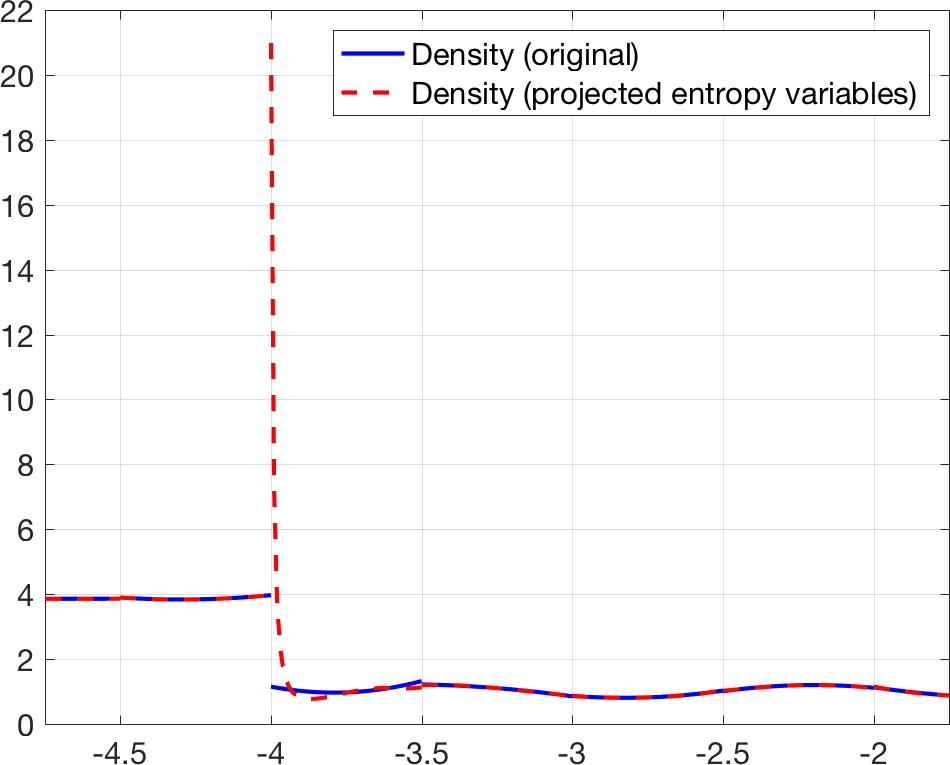
\includegraphics[width=.32\textwidth]{sineShockDensityCompare.png}}\label{subfig:u1}
\hspace{.1em}
\subfloat[$u(x)$ and $u\LRp{\Pi_N \bm{v}}$]{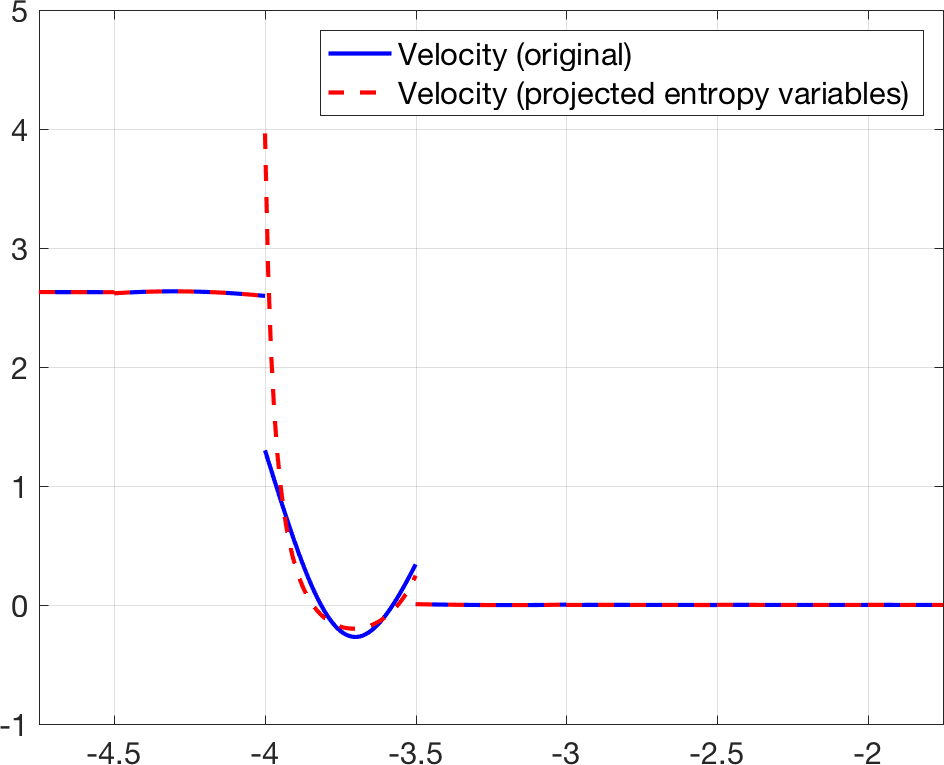
\includegraphics[width=.32\textwidth]{sineShockVelocityCompare.png}}\label{subfig:u2}
\hspace{.1em}
\subfloat[$p(x)$ and $p\LRp{\Pi_N \bm{v}}$]{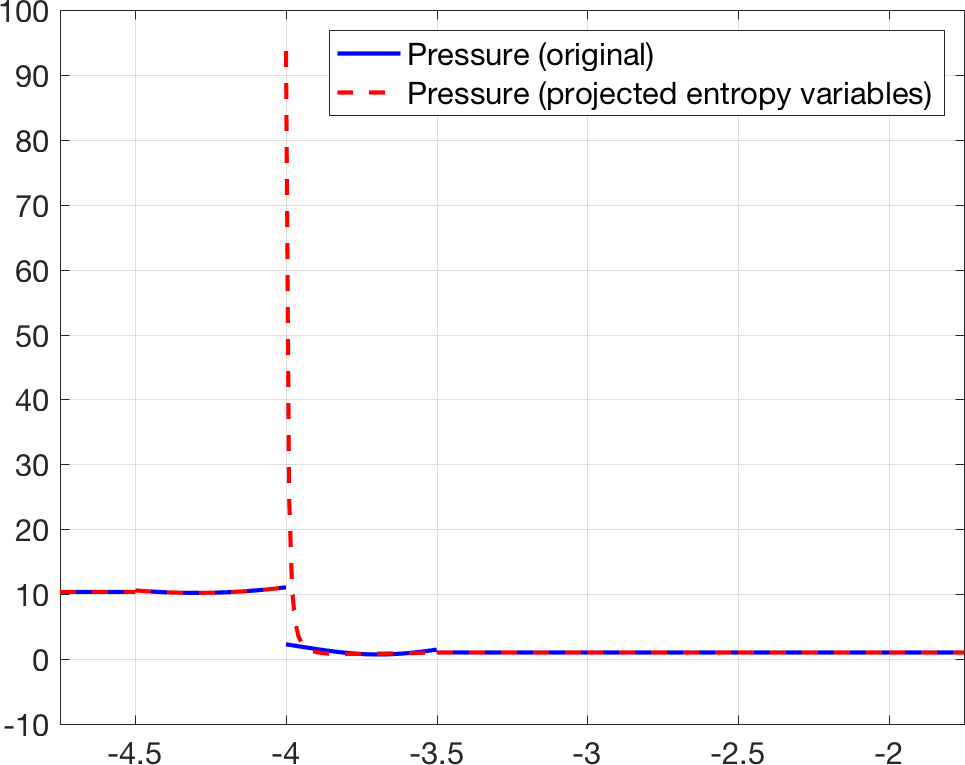
\includegraphics[width=.32\textwidth]{sineShockPressureCompare.png}}\label{subfig:u3}
\caption{Top row: comparisons of entropy variables (evaluated directly as functions of conservative variables) and projected entropy variables (using $N=2$, $K=20$ elements, and a GQ-$(N+2)$ quadrature rule) for the sine-shock interaction before the detection of negative density and pressures.  Bottom row: comparisons of the conservative variables and their evaluations in terms of the projected entropy variables. }
\label{fig:proj}
\end{figure}

Qualitatively similar behavior is observed when using a GQ-$(N+1)$ quadrature rule, though negative density and pressure values occur at a slightly later time.  In this case, the $L^2$ projection reduces to interpolation at interior Gauss points.  This still implies that $\bm{u}\LRp{\Pi_N\bm{v}}$ does not necessarily agree with $\bm{u}$ at element boundaries, and this discrepancy again leads to spikes in the conservative variables similar to those presented in Figure~\ref{fig:proj}.  These experiments suggest that the lack of control of boundary values in $\Pi_N \bm{v}$ leads to large oscillations or spikes in the boundary values of $\bm{u}\LRp{\Pi_N\bm{v}}$.  The presence of boundary nodes in GLL quadratures avoids this issue: $\bm{u}\LRp{\Pi_N\bm{v}}$ and $\bm{u}$ agree at element boundaries due to the fact that quadrature-based $L^2$ projection under a GLL quadrature is equivalent to interpolation at GLL points.  

This scenario illustrates some of the more subtle differences between the use of GLL and GQ quadratures.  We note that bound-preserving and TVD limiters \cite{zhang2010positivity, zhang2012maximum} are typically implemented in practice to detect and control spikes of the kind observed in these numerical experiments.  However, slope-limiting the conservative variables $\bm{u}$ may still result in spikes being generated when evaluating $\bm{u}\LRp{\Pi_N\bm{v}}$ (unless the slope is set to zero such that $\bm{u}$ is constant).  A more nuanced approach will likely require modifying the conservative variables $\bm{u}$ based on the projected entropy variables $\Pi_N \bm{v}$ to control oscillations while maintaining entropy conservation.  These strategies will be the focus in future work.  

\section{Conclusions}

This work presents a generalization of discretely entropy conservative methods from diagonal-norm SBP-DG methods to a more general class of high order DG methods, which include dense norm SBP operators and over-integrated quadrature rules.  The resulting schemes satisfy a discrete conservation of entropy while maintaining a reasonable computational cost and small stencil.  Numerical results indicate that the resulting methods deliver high order accuracy for smooth solutions while improving stability for under-resolved and shock solutions compared to non-entropy conservative and non-entropy stable solvers.  We also describe differences between the sensitivity of methods based on Gauss-Lobatto quadrature and methods based on Gauss quadrature rules.  

We note that, while entropy conservative and entropy stable schemes improve the robustness of solvers for nonlinear hyperbolic conservation laws, they do not address problems such as spurious oscillations in high order approximations of shock solutions or positivity preservation of density and pressure variables \cite{chen2017entropy}.  These issues can be addressed through the use of regularization (e.g.\ filtering, artificial viscosity) and/or limiting.  However, this can lead to a reliance on regularization techniques as ad-hoc stabilization mechanisms.  Addressing this issue requires constructing methods which avoid the need for excessive regularization and limiting in the pursuit of stability, and is a significant motivation for the development of entropy conservative and entropy stable discretizations.  

Finally, we note that the analysis and numerical experiments in this work are presented in one dimension for clarity and conciseness of presentation.  This work is intended as a foundation on which higher dimensional schemes can be constructed.  Future work will focus on generalizations to higher dimensions (including simplicial and pyramidal elements), as well as convergence and error analysis.  

\section{Acknowledgments}

The author thanks Lucas Wilcox, Andrew Winters, David M.\ Williams, Weifeng Qiu, and Paul Hand for helpful discussions.  Jesse Chan is supported by the National Science Foundation under awards DMS-1719818 and DMS-1712639.  

\appendix
\section{Assumptions on the flux function}
\label{appendix:A}

In this work, we assume that the flux function $\bm{f}_S$ admits an absolutely convergent expansion of the form
\[
\bm{f}_S(x,y) = \sum_{i=1}^{\infty} \bm{f}_i(x) \bm{g}_i(y), 
\]
where $\bm{f}_i, \bm{g}_i$ are real and bounded for appropriate values of $x,y$.  This holds, for example, for analytic $\bm{f}_S$, for which the Taylor series can be rearranged to yield the form of the desired expansion.  This assumption is trivially satisfied for the Burgers' and shallow water equations, as the flux functions consist only of finite sums of products of variables.  However, for the compressible Euler equations, this expansion is less clear due to the presence of the logarithmic mean in the entropy conservative Chandreshekar flux and the presence of inverses of averages and logarithmic means of the variable $\beta = \rho/(2p)$.  

%\note{For Burgers and shallow water, this sum is finite.  
%For the Chandreshekar flux, we consider individual components: the logarithmic mean $L(x,y)$ admits a convergent expansion and is analytic in $x$ \cite{mustonen2002logarithmic}.  CH's flux introduces rational denominators involving the mean and log-mean of $\beta = \rho/(2p)$, which is bounded away from zero if the density and temperature are bounded away from zero.  By composition and products of analytic functions, the CH flux is also analytic. }

We first address the logarithmic mean by noting that it can be expanded out into series form using multi-index notation \cite{mustonen2002logarithmic}.  Let $\mu= (\mu_1,\mu_2)$ be positive integers and define $\LRb{\mu} = \mu_1 + \mu_2$; then, the logarithmic mean can be rewritten as
\[
\frac{x - y}{\log(x)-\log(y)} = \sum_{n=0}^{\infty} \frac{x_n}{n!}, \qquad x_n = \sum_{\LRb{\mu} = n} \frac{\log(x)^{\mu_1}\log(y)^{\mu_2}}{n+1},
\]
where division by $(n+1)$ averages over the $(n+1)$ different permutations of $\mu_1,\mu_2 \geq 0$ which sum to $n$.  
Since $x_n$ is the average of degree $n$ powers of $\log(x),\log(y)$, we have that
\[
%\LRb{x_n} \leq \max{\LRb{\log(x)^n,\log(y)^n}}, \qquad 
\LRb{\frac{x_n}{n!}} \leq \frac{\max{\LRb{\log(x),\log(y)}}^n}{n!}. 
\]
The latter term is simply the $n$th term of the exponential Taylor series evaluated with the argument $\max{\LRb{\log(x),\log(y)}}$.  Because the exponential Taylor series converges absolutely everywhere, the series for the logarithmic mean also converges absolutely for $x,y$ bounded away from $0$ and $\infty$ (i.e.\ $x,y$ are in the logarithmic interval of convergence).  

The entropy conservative Chandreshekar flux also requires multiplication by the terms
\[
\frac{1}{\avg{\beta}}, \qquad \frac{1}{\avg{\beta}^{\log}}, \qquad \beta = \frac{\rho}{2p}.
\]
These terms are analytic if $\rho, p, \avg{\beta}, \avg{\beta}^{\log}$ are bounded away from zero as assumed in (\ref{eq:assumption2}).  Because the composition, sum, and product of analytic functions are also analytic, the Chandreshekar flux also is analytic under positivity assumptions.  

Finally, we note that the application of the operators $D_N, D^x_h$ to convergent infinite sums should be rigorously justified.  
This requires $D_N, D^x_h$ to be bounded operators mapping from a broken Sobolev space to $P^N$ or $V_h$, which can be shown using boundedness of local $L^2$ projection operators and discrete inverse and trace inequalities \cite{chan2015gpu}.   

\bibliographystyle{unsrt}
\bibliography{dg}


\end{document}


